\documentclass[10pt,a4paper,hidelinks]{article}
\usepackage[utf8]{inputenc}
\usepackage[english]{babel}
\usepackage[T1]{fontenc}

\newcommand{\documentStatus}{SUBMITTED}


\usepackage{amsmath}
\usepackage{amsfonts}
\usepackage{amssymb}
\usepackage{graphicx}
\usepackage{lmodern}
\usepackage{tikz}
\usetikzlibrary{positioning}
\usetikzlibrary{shapes,snakes}
\usepackage{epigraph} 
\usepackage[left=2.5cm,
            right=2.5cm,
            top=2cm,
            bottom=2cm]{geometry}
\usepackage{setspace}
\usepackage{caption}
\usepackage{subcaption}
\usepackage{epigraph}
\usepackage{pdflscape}
\usepackage{pgfplots}

\usepackage{titlesec}
\usepackage{tcolorbox}
\usepackage{background}
\usepackage{url}
\usepackage[pdfauthor={Pierre Jézégou},
            pdftitle={ADS assignement},
            pdfsubject={Word games},
            pdfkeywords={}]{hyperref}
\usepackage{wrapfig}

\backgroundsetup{contents=\documentStatus, color=\watermarkColor}

\usepackage{fancyhdr}
\usepackage{textpos}
\usepackage{sectsty}
\usepackage{xcolor}

\setlength{\parindent}{0pt}

%%%%%%%%%%%%%%% Colors %%%%%%%%%%%%%%%
\subsectionfont{\color{fib_red}}
\subsubsectionfont{\color{fib_red}}
\renewcommand\fbox{\fcolorbox{black}{fib_red!20}}

\definecolor{fib_red}{RGB}{191,21,64}
\definecolor{fib_gray}{RGB}{111,111,111}
\definecolor{blue_upc}{RGB}{52,120,186}

\usepackage{listings}
\lstdefinestyle{mystyle}{
  backgroundcolor=\color{gray!10},
  stringstyle=\color{green!50!black},
  keywordstyle=\color{fib_red},
  numberstyle=\tiny\color{fib_gray},
  commentstyle=\color{blue_upc},
  basicstyle=\ttfamily\footnotesize,
  breakatwhitespace=false,         
  breaklines=true,                 
  captionpos=b,                    
  keepspaces=true,                 
  numbers=left,                    
  numbersep=5pt,                  
  showspaces=false,                
  showstringspaces=false,
  showtabs=false,                  
  tabsize=2
}

\lstset{style=mystyle}

\usepackage[Bjornstrup]{fncychap}
\newcommand{\watermarkColor}{red!10}


\onehalfspacing


\newcommand\VRule[1][\arrayrulewidth]{\vrule width #1}
\usepackage{xcolor,colortbl}

\newtcolorbox{mybox}[1]{
    arc=5pt,
    boxrule=0pt,
    colback=#1,
    width=\linewidth,
    halign=left,
}

\newenvironment{framed}[3]{
    \vspace*{0.5em}
    \begin{mybox}{#3!10}
        \textbf{#1}:\hfill \textit{#2}\\
        \hrule\vspace*{1em}
}
{\end{mybox}}

\newenvironment{exercise_description}[1]{
    \begin{framed}{Exercise description}{#1}{orange}
}
{\end{framed}}

\newenvironment{summary}{
    \begin{framed}{Summary}{Section \thesection}{blue}
}
{\end{framed}}


\newcommand{\colorverb}[2]{\textcolor{#1}{\texttt{\detokenize{#2}}}}
\newcommand{\type}[1]{\colorverb{green!50!black}{#1}}
\newcommand{\code}[1]{\colorverb{green!50!black}{#1}}


\usepackage{lmodern}
\renewcommand*\familydefault{\sfdefault}


\fancyfoot[R]{\raisebox{-0.5\baselineskip}{
\includegraphics[scale=0.25]{images/logos/upc_logo.jpeg}}}

\begin{document}
\pagestyle{plain}
\backgroundsetup{contents=,color=red!30}
\pagecolor{white}

\begin{center}
    \color{red!50!white}
    \textbf{\huge{STATUT - \documentStatus}}
\end{center}

\vfill


\color{black}
\begin{center}
    
\includegraphics[height=2cm]{images/logos/upc_logo.jpeg} \\
    % \vfill
    % 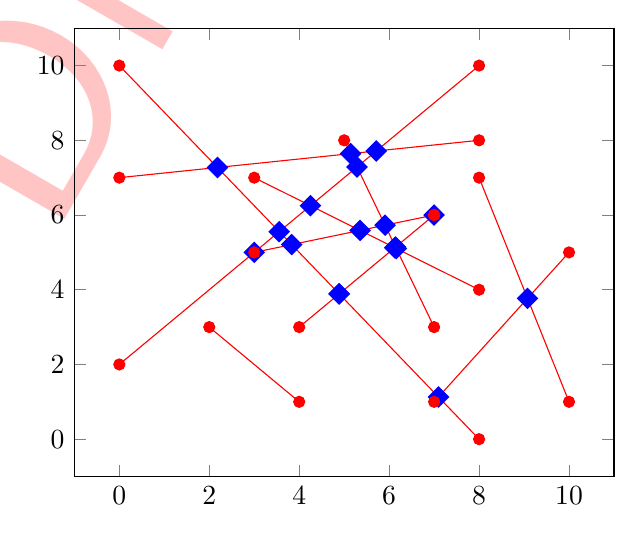
\begin{tikzpicture}
    \begin{axis}
        % Segments
        
            \addplot[red, mark=*] coordinates {(4, 3) (7, 6)};
        
            \addplot[red, mark=*] coordinates {(3, 5) (7, 6)};
        
            \addplot[red, mark=*] coordinates {(5, 8) (7, 3)};
        
            \addplot[red, mark=*] coordinates {(7, 1) (10, 5)};
        
            \addplot[red, mark=*] coordinates {(0, 7) (8, 8)};
        
            \addplot[red, mark=*] coordinates {(8, 7) (10, 1)};
        
            \addplot[red, mark=*] coordinates {(0, 2) (8, 10)};
        
            \addplot[red, mark=*] coordinates {(2, 3) (4, 1)};
        
            \addplot[red, mark=*] coordinates {(3, 7) (8, 4)};
        
            \addplot[red, mark=*] coordinates {(0, 10) (8, 0)};
        
        % Intersections
        
            \node[diamond,fill=blue, inner sep=2pt] at (axis cs:3.5555555555555554, 5.555555555555555) {};
        
            \node[diamond,fill=blue, inner sep=2pt] at (axis cs:4.888888888888889, 3.8888888888888884) {};
        
            \node[diamond,fill=blue, inner sep=2pt] at (axis cs:6.157894736842105, 5.105263157894737) {};
        
            \node[diamond,fill=blue, inner sep=2pt] at (axis cs:4.25, 6.25) {};
        
            \node[diamond,fill=blue, inner sep=2pt] at (axis cs:2.1818181818181817, 7.272727272727273) {};
        
            \node[diamond,fill=blue, inner sep=2pt] at (axis cs:4.888888888888889, 3.888888888888889) {};
        
            \node[diamond,fill=blue, inner sep=2pt] at (axis cs:7.096774193548387, 1.129032258064516) {};
        
            \node[diamond,fill=blue, inner sep=2pt] at (axis cs:3.8333333333333335, 5.208333333333333) {};
        
            \node[diamond,fill=blue, inner sep=2pt] at (axis cs:5.142857142857143, 7.642857142857143) {};
        
            \node[diamond,fill=blue, inner sep=2pt] at (axis cs:5.714285714285714, 7.714285714285714) {};
        
            \node[diamond,fill=blue, inner sep=2pt] at (axis cs:6.142857142857142, 5.142857142857143) {};
        
            \node[diamond,fill=blue, inner sep=2pt] at (axis cs:7.0, 6.0) {};
        
            \node[diamond,fill=blue, inner sep=2pt] at (axis cs:6.125, 5.125) {};
        
            \node[diamond,fill=blue, inner sep=2pt] at (axis cs:5.909090909090909, 5.7272727272727275) {};
        
            \node[diamond,fill=blue, inner sep=2pt] at (axis cs:5.285714285714286, 7.285714285714286) {};
        
            \node[diamond,fill=blue, inner sep=2pt] at (axis cs:9.076923076923077, 3.769230769230769) {};
        
            \node[diamond,fill=blue, inner sep=2pt] at (axis cs:5.352941176470589, 5.588235294117647) {};
        
            \node[diamond,fill=blue, inner sep=2pt] at (axis cs:3.0, 5.0) {};
        
    \end{axis}
\end{tikzpicture}

    \vfill
    \rule{\linewidth}{0.5mm} \\[1cm]
    {\Huge \textsc{\textcolor{fib_red}{Implementation of Sweep Lines}}}\\[1cm]
    {\Large \textsc{Assignment}}\\[0.4cm]
    {\huge \textsc{\textbf{Advanced data structures}}}\\[1cm]
    {\Large \textsc{Master in Research and Innovation - UPC}}\\[0.4cm]
    \rule{\linewidth}{0.5mm} \\[1.5cm]
\end{center}

\vfill

\textbf{Author:}
\begin{itemize}
\item Pierre \textsc{Jézégou}\newline
\textit{(Engineering student at École Centrale de Lille, Exchange student at UPC)}
\end{itemize}

\newpage
\color{black}
\pagecolor{white}
\pagestyle{fancy}
\tableofcontents

\section{Introduction}
\subsection{Sweep lines}
The Segment Intersection Problem is a classic problem in computational geometry. It involves finding all the intersections between a set of line segments in the plane. This problem has various applications, such as in computer graphics, robotics, and geographic information systems.\\

There are several algorithms to solve the Segment Intersection Problem, and one popular approach is the Sweep Line Algorithm. This algorithm involves sweeping a vertical line across the plane and processing the line segments as they are encountered by the sweep line.
To implement the Sweep Line Algorithm, we need to define the data structures and events that will be used. The data structures typically include a status structure to store the line segments which intersect the current sweep line position, and a priority queue to handle the events.\\
The events in the Sweep Line Algorithm correspond to the endpoints of the line segments. As the sweep line encounters an endpoint, it triggers an event that updates the status structure and performs any necessary computations.\\

By implementing the Sweep Line Algorithm, we can efficiently find all the intersections between the line segments and solve the Segment Intersection Problem.


\subsection{Project information}
All the source code (programs, documentation and image generators) is available in the GitHub respository dedicated to the project: \textbf{\url{https://github.com/pierre-jezegou/sweep-lines}}

For performance testing of algorithms, we use a MacBook Air with the M2 processor. This hardware provides ample computing power to execute our algorithms efficiently, ensuring swift analysis of their performance. As recommended, this report has been written in \LaTeX.


\subsection{Final example}
You can find below an example of the final result of the sweep line algorithm. This example is a mi-complex one with 12 segments. The algorithm is able to detect all the intersections between the segments. The result is plotted using the \code{tikz} package in \LaTeX.
\begin{figure}[h]
    \centering
    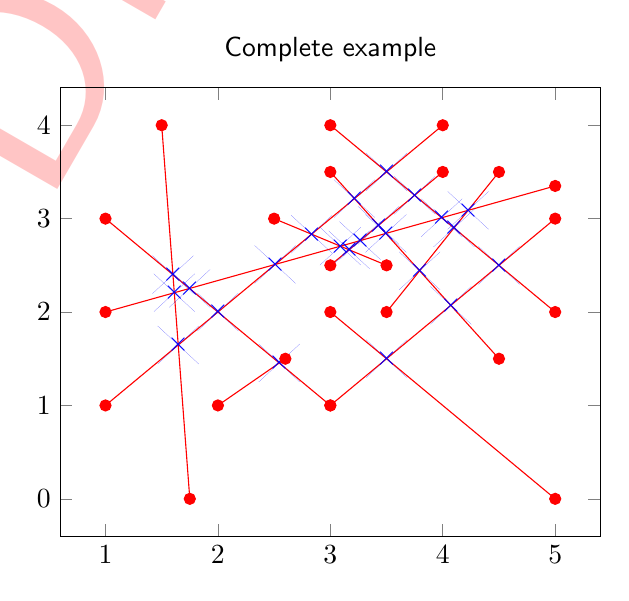
\begin{tikzpicture}
    \begin{axis}[title=Complete example]
        % Segments
        
            \addplot[red, mark=*] coordinates {(1, 1) (4, 4)};
        
            \addplot[red, mark=*] coordinates {(1, 3) (3, 1)};
        
            \addplot[red, mark=*] coordinates {(3, 1) (5, 3)};
        
            \addplot[red, mark=*] coordinates {(3, 2) (5, 0)};
        
            \addplot[red, mark=*] coordinates {(2, 1) (2.6, 1.5)};
        
            \addplot[red, mark=*] coordinates {(3, 4) (5, 2)};
        
            \addplot[red, mark=*] coordinates {(3, 3.5) (4.5, 1.5)};
        
            \addplot[red, mark=*] coordinates {(3.5, 2) (4.5, 3.5)};
        
            \addplot[red, mark=*] coordinates {(2.5, 3) (3.5, 2.5)};
        
            \addplot[red, mark=*] coordinates {(3, 2.5) (4, 3.5)};
        
            \addplot[red, mark=*] coordinates {(1.5, 4) (1.75, 0)};
        
            \addplot[red, mark=*] coordinates {(1, 2) (5, 3.35)};
        
        % Intersections
        
            \node[cross out, text=blue, fill=blue] at (axis cs:2.83333, 2.83333) {$\mathbf{\times}$};
        
            \node[cross out, text=blue, fill=blue] at (axis cs:4.5, 2.5) {$\mathbf{\times}$};
        
            \node[cross out, text=blue, fill=blue] at (axis cs:3.5, 3.5) {$\mathbf{\times}$};
        
            \node[cross out, text=blue, fill=blue] at (axis cs:2.0, 2.0) {$\mathbf{\times}$};
        
            \node[cross out, text=blue, fill=blue] at (axis cs:3.49377, 2.84165) {$\mathbf{\times}$};
        
            \node[cross out, text=blue, fill=blue] at (axis cs:3.16667, 2.66667) {$\mathbf{\times}$};
        
            \node[cross out, text=blue, fill=blue] at (axis cs:3.75, 3.25) {$\mathbf{\times}$};
        
            \node[cross out, text=blue, fill=blue] at (axis cs:1.74766, 2.25234) {$\mathbf{\times}$};
        
            \node[cross out, text=blue, fill=blue] at (axis cs:1.64706, 1.64706) {$\mathbf{\times}$};
        
            \node[cross out, text=blue, fill=blue] at (axis cs:1.6, 2.4) {$\mathbf{\times}$};
        
            \node[cross out, text=blue, fill=blue] at (axis cs:3.26415, 2.76415) {$\mathbf{\times}$};
        
            \node[cross out, text=blue, fill=blue] at (axis cs:3.99065, 3.00935) {$\mathbf{\times}$};
        
            \node[cross out, text=blue, fill=blue] at (axis cs:3.42857, 2.92857) {$\mathbf{\times}$};
        
            \node[cross out, text=blue, fill=blue] at (axis cs:4.1, 2.9) {$\mathbf{\times}$};
        
            \node[cross out, text=blue, fill=blue] at (axis cs:2.54545, 1.45455) {$\mathbf{\times}$};
        
            \node[cross out, text=blue, fill=blue] at (axis cs:3.08955, 2.70522) {$\mathbf{\times}$};
        
            \node[cross out, text=blue, fill=blue] at (axis cs:4.07143, 2.07143) {$\mathbf{\times}$};
        
            \node[cross out, text=blue, fill=blue] at (axis cs:1.61209, 2.20658) {$\mathbf{\times}$};
        
            \node[cross out, text=blue, fill=blue] at (axis cs:3.5, 1.5) {$\mathbf{\times}$};
        
            \node[cross out, text=blue, fill=blue] at (axis cs:2.50943, 2.50943) {$\mathbf{\times}$};
        
            \node[cross out, text=blue, fill=blue] at (axis cs:4.22581, 3.08871) {$\mathbf{\times}$};
        
            \node[cross out, text=blue, fill=blue] at (axis cs:3.79412, 2.44118) {$\mathbf{\times}$};
        
            \node[cross out, text=blue, fill=blue] at (axis cs:3.21429, 3.21429) {$\mathbf{\times}$};
        
    \end{axis}
\end{tikzpicture}
    \caption{Complete example}
\end{figure}

\section{Sweep Line Algorithm implementation}
\subsection{Structures}
To implement the Sweep Line Algorithm, you need to define the data structures that will be used. First, as the problem is in 2D, you need to define the Point and Segment classes. The Point class represents a point in the plane, while the Segment class represents a line segment defined by two endpoints.\\

The main data structures include the status structure and the event queue. The status structure stores the line segments that intersect the current sweep line position, while the event queue handles the events corresponding to the endpoints of the line segments.

\subsubsection{Point}
First of all, you have to define the \code{Point} class to represent a point in the plane. The Point class has two attributes, $x$ and $y$, representing the $x$ and $y$ coordinates of the point, respectively.
\begin{itemize}
    \item \code{x} (type: \type{float}): $x$ coordinate of the point.
    \item \code{y} (type: \type{float}): $y$ coordinate of the point.
\end{itemize}
\begin{figure}[h]
    \centering
    \begin{tikzpicture}
        \node[draw, rounded corners=2mm, inner sep = 0.2cm, fill=orange!0] { 
        \begin{tikzpicture} 
            \node[inner sep = 1mm] (title) { \Large{\bfseries Point }}; 
            % \draw (title.south west) -- (title.south east);
            \node[at=(title.south), anchor=north, inner sep=3mm, align=left, fill=green!30!black!10, yshift=-0.2cm] (attributes) {
                \begin{minipage}{60mm}
                    \textbf{Attributes}\\
                    \small{0}: \verb|x|\\
\small{1}: \verb|y|
                \end{minipage} 
                };
            % \draw (attributes.north west) -- (attributes.north east);
            \node[at=(attributes.south), anchor=north, inner sep=3mm, align=left, fill=blue!10, yshift=-0.2cm] (methods) {
                \begin{minipage}{60mm}
                    \textbf{Methods}\\
                    \small{0}: \verb|__eq__|\\
\small{1}: \verb|__hash__|\\
\small{2}: \verb|__init__|\\
\small{3}: \verb|__lt__|\\
\small{4}: \verb|__repr__|\\
\small{5}: \verb|format_point|\\
\small{6}: \verb|format_point_segment_pgf|
                \end{minipage} 
                };
            % \draw (methods.north west) -- (methods.north east);
        \end{tikzpicture}
        }; 
    \end{tikzpicture}
    \caption{Class description - Point }
    \label{class:Point}
\end{figure}
I also implemented classic methods to compare two points (\code{__lt__}, \code{__eq__}) or other to represent the point in pgf format.
\subsubsection{Segment}
The \code{Segment} class represents a line segment defined by two endpoints. The Segment class has two attributes, \code{start} and \code{end}, representing the two endpoints of the segment. I also implemented the \code{__lt__} method to compare two segments based on their $x$ and $y$ coordinates. Finally, there is a method to generate the code to represent the segment in pgf format
\begin{itemize}
    \item \code{start} (type: \type{Point}): Start point of the segment.
    \item \code{end} (type: \type{Point}): End point of the segment.
\end{itemize}
\begin{figure}[h]
    \centering
    \begin{tikzpicture}
        \node[draw, rounded corners=2mm, inner sep = 0.2cm, fill=orange!0] { 
        \begin{tikzpicture} 
            \node[inner sep = 1mm] (title) { \Large{\bfseries Segment }}; 
            % \draw (title.south west) -- (title.south east);
            \node[at=(title.south), anchor=north, inner sep=3mm, align=left, fill=green!30!black!10, yshift=-0.2cm] (attributes) {
                \begin{minipage}{60mm}
                    \textbf{Attributes}\\
                    \small{0}: \verb|start|\\
\small{1}: \verb|end|
                \end{minipage} 
                };
            % \draw (attributes.north west) -- (attributes.north east);
            \node[at=(attributes.south), anchor=north, inner sep=3mm, align=left, fill=blue!10, yshift=-0.2cm] (methods) {
                \begin{minipage}{60mm}
                    \textbf{Methods}\\
                    \small{0}: \verb|__eq__|\\
\small{1}: \verb|__init__|\\
\small{2}: \verb|__lt__|\\
\small{3}: \verb|__repr__|\\
\small{4}: \verb|current_y|\\
\small{5}: \verb|segment_to_pgf|
                \end{minipage} 
                };
            % \draw (methods.north west) -- (methods.north east);
        \end{tikzpicture}
        }; 
    \end{tikzpicture}
    \caption{Class description - Segment }
    \label{class:Segment}
\end{figure}

\subsubsection{Event}
As the sweep line encounters the endpoints of the line segments, it triggers events that update the status structure and perform any necessary computations. The Event class represents an event corresponding to an endpoint of a line segment. The Event class has three attributes:
\begin{itemize}
    \item \code{point} (type: \type{Point}): The point corresponding to the event.
    \item \code{segment} (type: \type{Segment}): The segment corresponding to the event.
    \item \code{type} (type: \type{str}): The type of the event, either "start" or "end".
\end{itemize}
There is one more attribute to store the two segments in case of an intersection event.
\begin{figure}[h]
    \centering
    \begin{tikzpicture}
        \node[draw, rounded corners=2mm, inner sep = 0.2cm, fill=orange!0] { 
        \begin{tikzpicture} 
            \node[inner sep = 1mm] (title) { \Large{\bfseries Event }}; 
            % \draw (title.south west) -- (title.south east);
            \node[at=(title.south), anchor=north, inner sep=3mm, align=left, fill=green!30!black!10, yshift=-0.2cm] (attributes) {
                \begin{minipage}{60mm}
                    \textbf{Attributes}\\
                    \small{0}: \verb|point|\\
\small{1}: \verb|segment|\\
\small{2}: \verb|event_type|\\
\small{3}: \verb|intersection_segments|
                \end{minipage} 
                };
            % \draw (attributes.north west) -- (attributes.north east);
            \node[at=(attributes.south), anchor=north, inner sep=3mm, align=left, fill=blue!10, yshift=-0.2cm] (methods) {
                \begin{minipage}{60mm}
                    \textbf{Methods}\\
                    \small{0}: \verb|__eq__|\\
\small{1}: \verb|__hash__|\\
\small{2}: \verb|__init__|\\
\small{3}: \verb|__lt__|\\
\small{4}: \verb|__repr__|
                \end{minipage} 
                };
            % \draw (methods.north west) -- (methods.north east);
        \end{tikzpicture}
        }; 
    \end{tikzpicture}
    \caption{Class description - Event }
    \label{class:Event}
\end{figure}

\subsubsection{Status and EventQueue}
In the implementation of the sweep line algorithm to find intersection points of line segments, I chose to use a heap for the event queue and a \code{SortedList} for the active segments to optimize performance and ensure efficient data management.\\

The heap, implemented using Python's \code{heapq} module, is ideal for the event queue because it allows for efficient extraction of the smallest element, which corresponds to the next event in the sweep line process. The heap provides $O(\log n)$ time complexity for both insertion and extraction, which is crucial for maintaining performance as we dynamically add and remove events.\\

For the active segments, the \code{SortedList} from the \code{sortedcontainers} module is used because it maintains the segments in a sorted order based on their y-coordinates at the current x-coordinate of the sweep line. This is essential for quickly finding and updating the relative order of segments, detecting intersections, and handling segment endpoints efficiently. The \code{SortedList} supports $O(\log n)$ insertion, deletion, and search operations, which significantly enhances the algorithm's efficiency compared to a naive list implementation.\\

By using a heap for the event queue and a \code{SortedList} for the active segments, the sweep line algorithm can efficiently manage the dynamic nature of events and maintain the correct order of segments, leading to an overall optimal performance in detecting intersections.


\subsection{Intersection}
To compute the intersection of two line segments, I define a function \code{segment_intersection(segment1, segment2)} that uses the parametric form of the segments. Each segment is represented by its start and end points. Let $(x_1, y_1)$ and $(x_2, y_2)$ be the coordinates of the start and end points of $\mathbf{P}$, the first segment, and $(x_3, y_3)$ and $(x_4, y_4)$ be the coordinates of the start and end points of $\mathbf{Q}$, the second segment.

Using the parametric equations:
$$\mathbf{P}(t) = (x_1 + t(x_2 - x_1), y_1 + t(y_2 - y_1))$$
$$\mathbf{Q}(u) = (x_3 + u(x_4 - x_3), y_3 + u(y_4 - y_3))$$

We find the intersection by solving:
$$\left\{\begin{array}{l}
    x_1 + t(x_2 - x_1) = x_3 + u(x_4 - x_3)\\
    y_1 + t(y_2 - y_1) = y_3 + u(y_4 - y_3)
\end{array}\right.$$

The determinant of the system is and if it is equal to 0, the lines are parallel and the function returns \code{False}. Otherwise, we compute the parameters $t$ and $u$:
$$\text{det} = (x_1 - x_2) \cdot (y_3 - y_4) - (y_1 - y_2) \cdot (x_3 - x_4)$$
If $\text{det} = 0$, the lines are parallel, and the function returns \code{False}.

If the lines are not parallel, we compute the parameters $t$ and $u$:
$$t = \frac{(x_1 - x_3) \cdot (y_3 - y_4) - (y_1 - y_3) \cdot (x_3 - x_4)}{\text{det}}$$
$$u = -\frac{(x_1 - x_2) \cdot (y_1 - y_3) - (y_1 - y_2) \cdot (x_1 - x_3)}{\text{det}}$$

The intersection point is valid if $0 \leq t \leq 1$ and $0 \leq u \leq 1$. The intersection coordinates are:
$$
\text{Point} = 
\begin{pmatrix}
    x_1 + t \cdot (x_2 - x_1)\\
    y_1 + t \cdot (y_2 - y_1)
\end{pmatrix}
$$
The function returns this intersection point as a \code{Point} object, rounded to five decimal places. If $t$ and $u$ are not within $[0, 1]$, the function returns \code{False}. Using the parametric form ensures an accurate computation of the intersection.

\subsection{Naive and semi-naive approach}
I implemented a totally naive approach to compute the intersection of two line segments. The naive approach involves checking all possible combinations of line segments to find the intersections. This approach is inefficient for large datasets but provides a baseline for comparison and validation of the sweep line algorithm's results. Indeed, the naive approach has a time complexity of $O(n^2)$, where $n$ is the number of line segments.\\

I chose to implement a semi-naive approach to compute the intersection of two line segments. The semi-naive approach involves checking all possible combinations of \textbf{active} line segments to find the intersections.

\subsection{Sweep line algorithm main parts}
The Sweep Line Algorithm consists of several key components that work together to find the intersections of line segments efficiently. The main parts of the algorithm include:
\begin{itemize}
    \item \textbf{Initialization}: The algorithm starts by initializing the event queue with the endpoints of the line segments and sorting them by their $x$-coordinates. The status structure is initialized as an empty \code{SortedList} to store the active segments.
    \lstinputlisting[language=Python, firstline=155, lastline=163]{../sweep_lines.py}
    \item \textbf{Event processing}: The algorithm processes the events in the event queue one by one as the sweep line moves from left to right. When an event is encountered, the algorithm updates the status structure and checks for intersections between the active segments.
    \lstinputlisting[language=Python, firstline=223, lastline=226]{../sweep_lines.py}
    \item \textbf{Intersection detection}: The algorithm detects intersections between the active segments by comparing adjacent segments in the status structure. If an intersection is found, the algorithm adds the intersection point to the event queue.
    \lstinputlisting[language=Python, firstline=165, lastline=178]{../sweep_lines.py}
    \item \textbf{Status structure update}: The algorithm updates the status structure by inserting or deleting segments based on the event type (start or end). The status structure is maintained in sorted order based on the segments' $y$-coordinates at the current $x$-coordinate of the sweep line.
    \lstinputlisting[language=Python, firstline=227, lastline=227]{../sweep_lines.py}
    \lstinputlisting[language=Python, firstline=246, lastline=246]{../sweep_lines.py}
\end{itemize}

\section{Tests and results}
First, I implemented all the code needed to plot directly the segments and the intersections. I used the \code{tikz} package to generate the plots. I also implemented a function to generate random segments and test the intersection function. The function generates a random dataset of line segments and computes the intersections using the sweep line algorithm. The results are plotted to visualize the intersections and validate the algorithm's correctness. This helps a lot to understand the algorithm and to debug it.

\subsection{Examples implementation}
Before trying to generate intersections for complex datasets, we first have to study some simple and also special cases. Indeed, we can have two segments that do not intersect, two segments that intersect at one point, or two segments that overlap...
\subsubsection{Colinear intersecting segments}
\begin{figure}[h!]
    \centering
    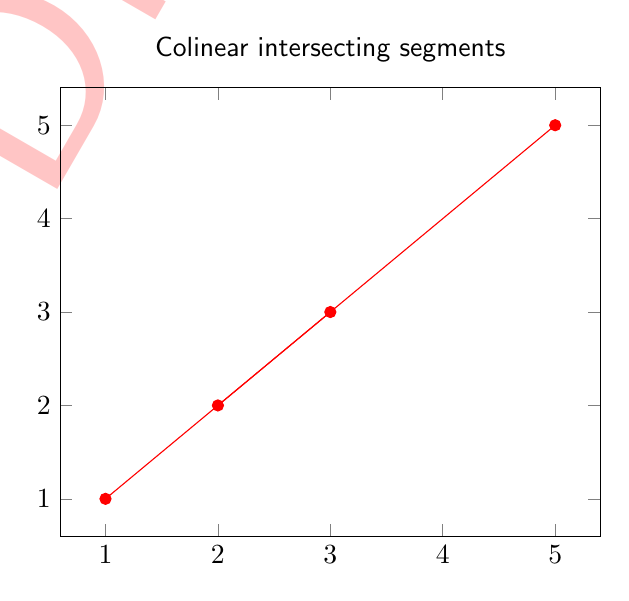
\begin{tikzpicture}
    \begin{axis}[title=Colinear intersecting segments]
        % Segments
        
            \addplot[red, mark=*] coordinates {(1, 1) (3, 3)};
        
            \addplot[red, mark=*] coordinates {(2, 2) (5, 5)};
        
        % Intersections
        
    \end{axis}
\end{tikzpicture}
    \caption{Colinear intersecting segments}
\end{figure}
When two segments are colinear, we can have three cases: the segments do not intersect, the segments intersect at one point, or the segments overlap. In the first case, the function returns \code{False}. In the second case, the function returns the intersection point. In the third case, my algorithm can't detect the intersection.

\subsubsection{Start is an end points of another segment}
\begin{figure}[h!]
    \centering
    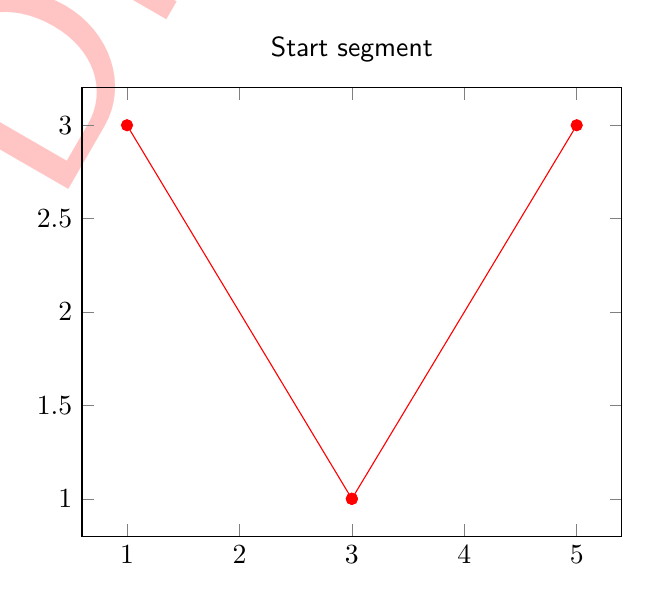
\begin{tikzpicture}
    \begin{axis}[title=Start segment = end other segment]
        % Segments
        
            \addplot[red, mark=*] coordinates {(1, 3) (3, 1)};
        
            \addplot[red, mark=*] coordinates {(3, 1) (5, 3)};
        
        % Intersections
        
    \end{axis}
\end{tikzpicture}
    \caption{Start is an end points of another segment}
\end{figure}
When the start point of a segment is an end point of another segment, I chose not to consider it as an intersection. Indeed, the segments are not intersecting, and the start point is not an intersection point. The function returns \code{False}. I chose this because I had problems in the priority of the events. Indeed, I prefred catching other intersections than completly obvious ones.

\subsubsection{Point belongs to the other segment}
\begin{figure}[h!]
    \centering
    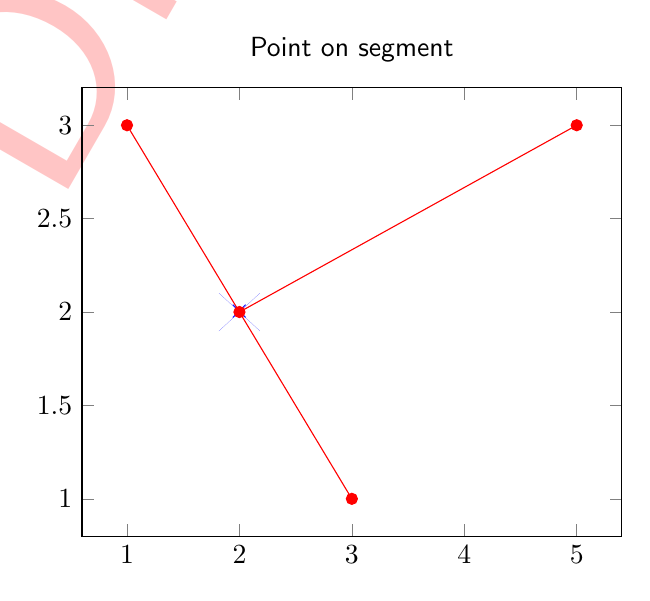
\begin{tikzpicture}
    \begin{axis}[title=Point on segment]
        % Segments
        
            \addplot[red, mark=*] coordinates {(1, 3) (3, 1)};
        
            \addplot[red, mark=*] coordinates {(2, 2) (5, 3)};
        
        % Intersections
        
            \node[cross out, text=blue, fill=blue] at (axis cs:2.0, 2.0) {$\mathbf{\times}$};
        
    \end{axis}
\end{tikzpicture}
    \caption{Point belongs to the other segment}
\end{figure}
When a point belongs to the other segment, this is clearly an intersection. The function returns the intersection point.

\subsubsection{Complexe case}
I generated a random dataset of 12 segments to test the intersection function. The results show that the function can accurately detect the intersections between the line segments and return the correct intersection points (except obvious ones). The function has been tested for various cases, including colinear segments, intersecting segments, and non-intersecting segments, but not has produced accurate results in all cases.
\begin{figure}[h]
    \centering
    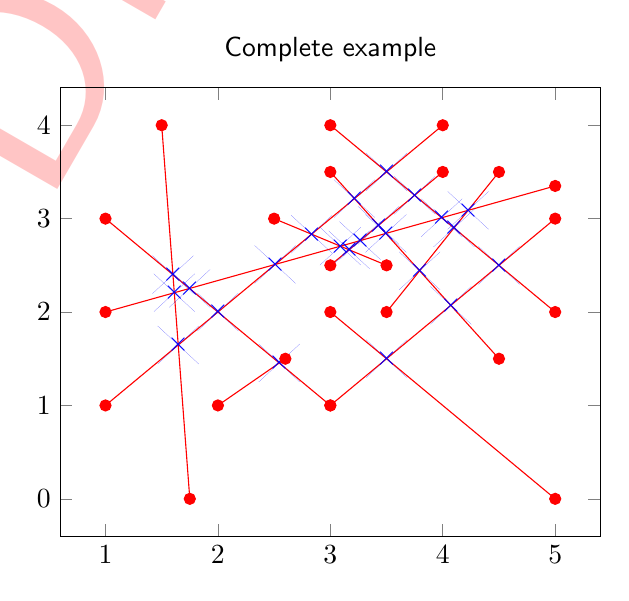
\begin{tikzpicture}
    \begin{axis}[title=Complete example]
        % Segments
        
            \addplot[red, mark=*] coordinates {(1, 1) (4, 4)};
        
            \addplot[red, mark=*] coordinates {(1, 3) (3, 1)};
        
            \addplot[red, mark=*] coordinates {(3, 1) (5, 3)};
        
            \addplot[red, mark=*] coordinates {(3, 2) (5, 0)};
        
            \addplot[red, mark=*] coordinates {(2, 1) (2.6, 1.5)};
        
            \addplot[red, mark=*] coordinates {(3, 4) (5, 2)};
        
            \addplot[red, mark=*] coordinates {(3, 3.5) (4.5, 1.5)};
        
            \addplot[red, mark=*] coordinates {(3.5, 2) (4.5, 3.5)};
        
            \addplot[red, mark=*] coordinates {(2.5, 3) (3.5, 2.5)};
        
            \addplot[red, mark=*] coordinates {(3, 2.5) (4, 3.5)};
        
            \addplot[red, mark=*] coordinates {(1.5, 4) (1.75, 0)};
        
            \addplot[red, mark=*] coordinates {(1, 2) (5, 3.35)};
        
        % Intersections
        
            \node[cross out, text=blue, fill=blue] at (axis cs:2.83333, 2.83333) {$\mathbf{\times}$};
        
            \node[cross out, text=blue, fill=blue] at (axis cs:4.5, 2.5) {$\mathbf{\times}$};
        
            \node[cross out, text=blue, fill=blue] at (axis cs:3.5, 3.5) {$\mathbf{\times}$};
        
            \node[cross out, text=blue, fill=blue] at (axis cs:2.0, 2.0) {$\mathbf{\times}$};
        
            \node[cross out, text=blue, fill=blue] at (axis cs:3.49377, 2.84165) {$\mathbf{\times}$};
        
            \node[cross out, text=blue, fill=blue] at (axis cs:3.16667, 2.66667) {$\mathbf{\times}$};
        
            \node[cross out, text=blue, fill=blue] at (axis cs:3.75, 3.25) {$\mathbf{\times}$};
        
            \node[cross out, text=blue, fill=blue] at (axis cs:1.74766, 2.25234) {$\mathbf{\times}$};
        
            \node[cross out, text=blue, fill=blue] at (axis cs:1.64706, 1.64706) {$\mathbf{\times}$};
        
            \node[cross out, text=blue, fill=blue] at (axis cs:1.6, 2.4) {$\mathbf{\times}$};
        
            \node[cross out, text=blue, fill=blue] at (axis cs:3.26415, 2.76415) {$\mathbf{\times}$};
        
            \node[cross out, text=blue, fill=blue] at (axis cs:3.99065, 3.00935) {$\mathbf{\times}$};
        
            \node[cross out, text=blue, fill=blue] at (axis cs:3.42857, 2.92857) {$\mathbf{\times}$};
        
            \node[cross out, text=blue, fill=blue] at (axis cs:4.1, 2.9) {$\mathbf{\times}$};
        
            \node[cross out, text=blue, fill=blue] at (axis cs:2.54545, 1.45455) {$\mathbf{\times}$};
        
            \node[cross out, text=blue, fill=blue] at (axis cs:3.08955, 2.70522) {$\mathbf{\times}$};
        
            \node[cross out, text=blue, fill=blue] at (axis cs:4.07143, 2.07143) {$\mathbf{\times}$};
        
            \node[cross out, text=blue, fill=blue] at (axis cs:1.61209, 2.20658) {$\mathbf{\times}$};
        
            \node[cross out, text=blue, fill=blue] at (axis cs:3.5, 1.5) {$\mathbf{\times}$};
        
            \node[cross out, text=blue, fill=blue] at (axis cs:2.50943, 2.50943) {$\mathbf{\times}$};
        
            \node[cross out, text=blue, fill=blue] at (axis cs:4.22581, 3.08871) {$\mathbf{\times}$};
        
            \node[cross out, text=blue, fill=blue] at (axis cs:3.79412, 2.44118) {$\mathbf{\times}$};
        
            \node[cross out, text=blue, fill=blue] at (axis cs:3.21429, 3.21429) {$\mathbf{\times}$};
        
    \end{axis}
\end{tikzpicture}
    \caption{Complete example}
\end{figure}

\subsection{Performance tests}
\subsubsection{CPU time}
First, we measure the CPU time taken by the sweep line algorithm to find the intersections of a set of random line segments. The CPU time is measured using the \code{time.process_time()} function, which returns the CPU time in seconds. The performance tests are conducted for different numbers of line segments to evaluate the scalability of the algorithm. The results show that the CPU time increases linearly with the number of line segments, indicating that the algorithm has a time complexity of $O(n \log n)$.

\begin{figure}[h]
    \centering
    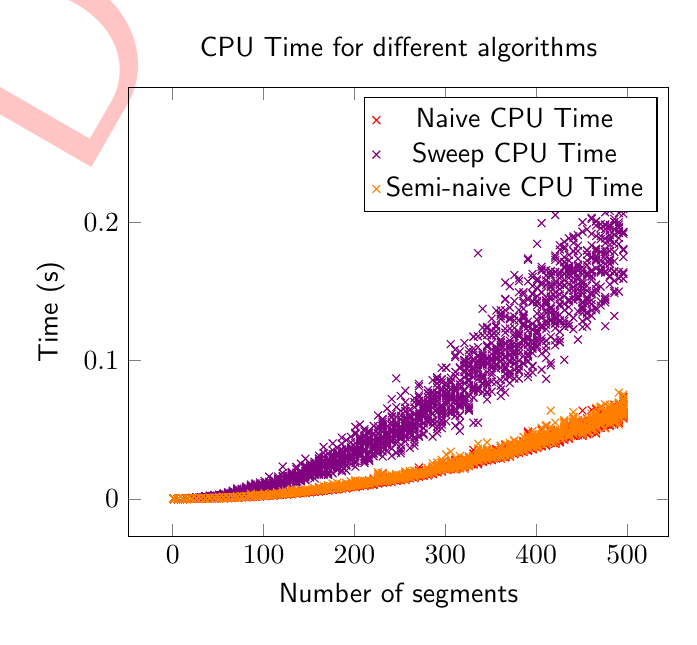
\begin{tikzpicture}
\begin{axis}[
    title={ CPU Time for different algorithms},
    xlabel={ Number of segments },
    ylabel={ Time (s) }
]

            \addplot[only marks, mark=x, color=red] coordinates {
            (1, 1.000000000001e-06)
(1, 1.000000000001e-06)
(1, 1.000000000001e-06)
(1, 9.999999999940612e-07)
(1, 0.0)
(1, 0.0)
(1, 0.0)
(1, 1.000000000001e-06)
(1, 1.000000000001e-06)
(1, 0.0)
(1, 0.0)
(1, 0.0)
(1, 0.0)
(1, 0.0)
(1, 0.0)
(1, 9.999999999940612e-07)
(1, 1.000000000001e-06)
(1, 2.000000000002e-06)
(1, 1.000000000001e-06)
(1, 0.0)
(6, 8.000000000001062e-06)
(6, 8.999999999995123e-06)
(6, 8.000000000001062e-06)
(6, 9.000000000002062e-06)
(6, 5.999999999999062e-06)
(6, 5.999999999999062e-06)
(6, 8.000000000001062e-06)
(6, 1.0999999999997123e-05)
(6, 9.000000000002062e-06)
(6, 8.000000000001062e-06)
(6, 8.000000000001062e-06)
(6, 7.000000000000062e-06)
(6, 7.000000000000062e-06)
(6, 7.000000000000062e-06)
(6, 8.999999999995123e-06)
(6, 1.0000000000003062e-05)
(6, 7.000000000000062e-06)
(6, 7.000000000000062e-06)
(6, 9.000000000002062e-06)
(6, 8.999999999995123e-06)
(11, 2.4999999999997247e-05)
(11, 2.1999999999994246e-05)
(11, 2.2999999999995246e-05)
(11, 2.8000000000000247e-05)
(11, 2.2000000000008124e-05)
(11, 2.8000000000000247e-05)
(11, 3.300000000000525e-05)
(11, 2.2999999999995246e-05)
(11, 2.6999999999999247e-05)
(11, 3.200000000000425e-05)
(11, 3.899999999999737e-05)
(11, 3.299999999999137e-05)
(11, 3.200000000000425e-05)
(11, 3.900000000001125e-05)
(11, 1.8999999999991246e-05)
(11, 4.200000000000037e-05)
(11, 2.9000000000001247e-05)
(11, 3.699999999999537e-05)
(11, 2.8000000000000247e-05)
(11, 2.2999999999995246e-05)
(16, 5.9999999999990616e-05)
(16, 5.8999999999989616e-05)
(16, 5.9000000000003494e-05)
(16, 5.8000000000002494e-05)
(16, 6.0000000000004494e-05)
(16, 5.8000000000002494e-05)
(16, 4.700000000000537e-05)
(16, 6.199999999999262e-05)
(16, 5.8000000000002494e-05)
(16, 5.7000000000001494e-05)
(16, 4.600000000000437e-05)
(16, 4.999999999999449e-05)
(16, 4.400000000000237e-05)
(16, 5.4999999999999494e-05)
(16, 6.0999999999991616e-05)
(16, 6.499999999999562e-05)
(16, 6.20000000000065e-05)
(16, 5.7999999999988616e-05)
(16, 6.399999999999462e-05)
(16, 6.0999999999991616e-05)
(21, 0.00010800000000001087)
(21, 9.800000000000086e-05)
(21, 9.299999999999586e-05)
(21, 9.699999999999986e-05)
(21, 0.00010399999999999299)
(21, 9.299999999999586e-05)
(21, 0.00011300000000000199)
(21, 0.00010000000000000286)
(21, 9.799999999998699e-05)
(21, 9.500000000001174e-05)
(21, 0.00011700000000000599)
(21, 0.00010899999999999799)
(21, 9.299999999999586e-05)
(21, 0.00010400000000000686)
(21, 8.299999999999974e-05)
(21, 9.399999999999686e-05)
(21, 8.800000000000474e-05)
(21, 9.199999999999486e-05)
(21, 0.00010799999999999699)
(21, 8.099999999999774e-05)
(26, 0.00015800000000000536)
(26, 0.00013399999999999523)
(26, 0.00014799999999999536)
(26, 0.00014400000000000523)
(26, 0.00014499999999999236)
(26, 0.0001290000000000041)
(26, 0.00014700000000000824)
(26, 0.00013900000000000023)
(26, 0.00014700000000000824)
(26, 0.00014199999999998936)
(26, 0.00014200000000000323)
(26, 0.0001789999999999986)
(26, 0.0001290000000000041)
(26, 0.0001260000000000011)
(26, 0.00014600000000000724)
(26, 0.00013999999999998736)
(26, 0.00016199999999999548)
(26, 0.00014899999999999636)
(26, 0.00013799999999999923)
(26, 0.0001310000000000061)
(31, 0.00019800000000000373)
(31, 0.00022600000000000398)
(31, 0.00020000000000000573)
(31, 0.0002459999999999962)
(31, 0.00020100000000000673)
(31, 0.0001689999999999886)
(31, 0.0001840000000000036)
(31, 0.0001729999999999926)
(31, 0.00021899999999999697)
(31, 0.0001870000000000066)
(31, 0.0001789999999999986)
(31, 0.00017800000000001148)
(31, 0.00020399999999998197)
(31, 0.00018899999999999473)
(31, 0.00019600000000000173)
(31, 0.00020899999999998697)
(31, 0.00018600000000001948)
(31, 0.00021899999999999697)
(31, 0.00018599999999999173)
(31, 0.00021499999999999297)
(36, 0.00027499999999999747)
(36, 0.0002520000000000022)
(36, 0.00027399999999999647)
(36, 0.0003499999999999892)
(36, 0.0002680000000000182)
(36, 0.0003389999999999782)
(36, 0.00032699999999999396)
(36, 0.00024199999999999222)
(36, 0.00026799999999999047)
(36, 0.0002859999999999807)
(36, 0.0002969999999999917)
(36, 0.0002570000000000072)
(36, 0.0002849999999999797)
(36, 0.00023600000000001398)
(36, 0.0002530000000000032)
(36, 0.0003009999999999957)
(36, 0.0003170000000000117)
(36, 0.000246000000000024)
(36, 0.0002449999999999952)
(36, 0.0002580000000000082)
(41, 0.00038099999999999246)
(41, 0.00032699999999999396)
(41, 0.00043699999999999295)
(41, 0.0003569999999999962)
(41, 0.00033700000000000396)
(41, 0.00034200000000000896)
(41, 0.0003220000000000167)
(41, 0.00032999999999999696)
(41, 0.0003720000000000112)
(41, 0.0004300000000000137)
(41, 0.00039900000000001046)
(41, 0.0003610000000000002)
(41, 0.00036999999999998145)
(41, 0.0003660000000000052)
(41, 0.00033299999999999996)
(41, 0.0003790000000000182)
(41, 0.0004089999999999927)
(41, 0.00033500000000000196)
(41, 0.0003509999999999902)
(41, 0.00032899999999999596)
(46, 0.0004790000000000072)
(46, 0.0004860000000000142)
(46, 0.0005390000000000117)
(46, 0.0004920000000000202)
(46, 0.0004790000000000072)
(46, 0.0005140000000000144)
(46, 0.00046100000000001695)
(46, 0.0004949999999999954)
(46, 0.00044700000000000295)
(46, 0.0004190000000000027)
(46, 0.00046000000000001595)
(46, 0.0004730000000000012)
(46, 0.0005410000000000137)
(46, 0.00040399999999995995)
(46, 0.00044399999999999995)
(46, 0.00043999999999999595)
(46, 0.0005049999999999777)
(46, 0.0004830000000000112)
(46, 0.00042399999999997995)
(46, 0.00047399999999997444)
(51, 0.0005799999999999694)
(51, 0.0005589999999999762)
(51, 0.0004870000000000152)
(51, 0.0005909999999999527)
(51, 0.0005209999999999937)
(51, 0.0005109999999999837)
(51, 0.0005879999999999774)
(51, 0.0006189999999999807)
(51, 0.0005359999999999809)
(51, 0.0005809999999999982)
(51, 0.0005100000000000104)
(51, 0.0005140000000000144)
(51, 0.0005370000000000097)
(51, 0.0005090000000000372)
(51, 0.0006519999999999859)
(51, 0.0005330000000000057)
(51, 0.0006329999999999947)
(51, 0.0005489999999999662)
(51, 0.0004769999999999497)
(51, 0.0005609999999999782)
(56, 0.0006399999999999739)
(56, 0.0006869999999999932)
(56, 0.0006760000000000099)
(56, 0.0006809999999999872)
(56, 0.0007199999999999984)
(56, 0.0006889999999999952)
(56, 0.0005890000000000062)
(56, 0.0006349999999999967)
(56, 0.0007830000000000337)
(56, 0.0006300000000000194)
(56, 0.0005840000000000289)
(56, 0.0006929999999999992)
(56, 0.0006399999999999739)
(56, 0.0006770000000000387)
(56, 0.0006829999999999892)
(56, 0.0007050000000000112)
(56, 0.0006140000000000034)
(56, 0.0006750000000000367)
(56, 0.0007110000000000172)
(56, 0.0006610000000000227)
(61, 0.0007179999999999964)
(61, 0.0009009999999999851)
(61, 0.0007820000000000049)
(61, 0.0008640000000000314)
(61, 0.0007809999999999762)
(61, 0.0008340000000000014)
(61, 0.0008279999999999954)
(61, 0.0007730000000000237)
(61, 0.0007880000000000109)
(61, 0.0007709999999999662)
(61, 0.0007869999999999822)
(61, 0.0009210000000000607)
(61, 0.0008159999999999279)
(61, 0.0007859999999999534)
(61, 0.0009029999999999871)
(61, 0.0008020000000000804)
(61, 0.0007779999999999454)
(61, 0.0008159999999999279)
(61, 0.0008460000000000134)
(61, 0.0007570000000000077)
(66, 0.0008029999999999982)
(66, 0.0008940000000000614)
(66, 0.0010569999999999746)
(66, 0.0008779999999999344)
(66, 0.0010539999999999994)
(66, 0.0009419999999999984)
(66, 0.0009569999999999856)
(66, 0.0008810000000000207)
(66, 0.0009630000000000472)
(66, 0.0008810000000000207)
(66, 0.0008580000000000254)
(66, 0.0008949999999999791)
(66, 0.0009259999999999824)
(66, 0.0009460000000000024)
(66, 0.0008479999999999599)
(66, 0.0012839999999999518)
(66, 0.0010169999999999346)
(66, 0.0011459999999999804)
(66, 0.0010369999999999546)
(66, 0.0009850000000000136)
(71, 0.0010689999999999866)
(71, 0.0010670000000000401)
(71, 0.0012349999999999861)
(71, 0.0013490000000000446)
(71, 0.0010690000000000976)
(71, 0.001190999999999942)
(71, 0.0012159999999999949)
(71, 0.0010879999999999779)
(71, 0.0009689999999999976)
(71, 0.0010639999999999539)
(71, 0.0010349999999998971)
(71, 0.0010740000000000194)
(71, 0.0010489999999999666)
(71, 0.0010999999999999899)
(71, 0.0012099999999999334)
(71, 0.0010069999999999801)
(71, 0.0011710000000000331)
(71, 0.0011020000000000474)
(71, 0.0010360000000000369)
(71, 0.0009749999999999481)
(76, 0.001466999999999996)
(76, 0.0011409999999999476)
(76, 0.0014450000000000296)
(76, 0.0011619999999999964)
(76, 0.0017880000000000118)
(76, 0.0011919999999999709)
(76, 0.0013250000000000206)
(76, 0.001415000000000055)
(76, 0.0013690000000000646)
(76, 0.0013819999999999943)
(76, 0.0012759999999999438)
(76, 0.0011539999999999884)
(76, 0.0011219999999999564)
(76, 0.0011719999999999509)
(76, 0.0013260000000000494)
(76, 0.0013020000000000254)
(76, 0.0012409999999999366)
(76, 0.001371000000000011)
(76, 0.0013699999999999823)
(76, 0.0013250000000000206)
(81, 0.0015609999999999236)
(81, 0.001534999999999953)
(81, 0.0014879999999999338)
(81, 0.0013490000000000446)
(81, 0.001527000000000056)
(81, 0.0013780000000001014)
(81, 0.001526999999999834)
(81, 0.0017810000000000326)
(81, 0.0013190000000000701)
(81, 0.0012690000000001866)
(81, 0.001554999999999973)
(81, 0.0015849999999999476)
(81, 0.0015959999999999308)
(81, 0.0016160000000000618)
(81, 0.001519000000000048)
(81, 0.0015810000000000546)
(81, 0.0015039999999999498)
(81, 0.0013019999999999143)
(81, 0.0014990000000001391)
(81, 0.0014359999999999928)
(86, 0.001919000000000004)
(86, 0.0018020000000000813)
(86, 0.0017300000000000093)
(86, 0.0016959999999999198)
(86, 0.0017800000000001148)
(86, 0.0014410000000000256)
(86, 0.0018249999999999655)
(86, 0.0016920000000000268)
(86, 0.0017209999999998615)
(86, 0.001654999999999962)
(86, 0.001723000000000141)
(86, 0.0016490000000000116)
(86, 0.0014100000000001334)
(86, 0.0016699999999998383)
(86, 0.0017059999999999853)
(86, 0.0017759999999999998)
(86, 0.0016460000000000363)
(86, 0.0016519999999999868)
(86, 0.0017730000000000246)
(86, 0.0016220000000000123)
(91, 0.0017560000000000908)
(91, 0.0016819999999999613)
(91, 0.001851000000000047)
(91, 0.0018329999999999735)
(91, 0.0018460000000000143)
(91, 0.0020050000000000345)
(91, 0.0018210000000000726)
(91, 0.0019769999999998955)
(91, 0.001775000000000082)
(91, 0.0018149999999999)
(91, 0.001819000000000015)
(91, 0.0019770000000001176)
(91, 0.0021879999999998567)
(91, 0.0018700000000000383)
(91, 0.0018799999999998818)
(91, 0.001870999999999956)
(91, 0.0019329999999999625)
(91, 0.0019089999999999385)
(91, 0.0019160000000000288)
(91, 0.0019370000000000775)
(96, 0.0023920000000001718)
(96, 0.002170999999999923)
(96, 0.0020100000000000673)
(96, 0.0019370000000000775)
(96, 0.0019940000000000513)
(96, 0.001878999999999964)
(96, 0.002131000000000105)
(96, 0.001910999999999996)
(96, 0.001956000000000069)
(96, 0.00231899999999996)
(96, 0.0021930000000001115)
(96, 0.0018739999999999313)
(96, 0.0020700000000000163)
(96, 0.0019599999999999618)
(96, 0.0020739999999999092)
(96, 0.0020130000000000425)
(96, 0.0021450000000000635)
(96, 0.002059000000000033)
(96, 0.0020780000000000243)
(96, 0.0020890000000000075)
(101, 0.0024249999999998995)
(101, 0.0020530000000000825)
(101, 0.002333999999999836)
(101, 0.0021539999999999893)
(101, 0.0022180000000000533)
(101, 0.002275000000000027)
(101, 0.0022379999999999622)
(101, 0.0023089999999998945)
(101, 0.0022249999999999215)
(101, 0.002151000000000014)
(101, 0.0022580000000003153)
(101, 0.002473999999999865)
(101, 0.002531000000000283)
(101, 0.0024169999999998915)
(101, 0.002235000000000209)
(101, 0.0021900000000001363)
(101, 0.0021049999999998015)
(101, 0.0022690000000000765)
(101, 0.002395000000000369)
(101, 0.0020889999999997855)
(106, 0.00271100000000013)
(106, 0.0026130000000001985)
(106, 0.0024609999999998244)
(106, 0.0025780000000001912)
(106, 0.0023320000000000007)
(106, 0.0025599999999998957)
(106, 0.002587000000000117)
(106, 0.0025439999999998797)
(106, 0.0025330000000001185)
(106, 0.002362999999999893)
(106, 0.0026999999999999247)
(106, 0.0023539999999999672)
(106, 0.002670999999999868)
(106, 0.0025800000000000267)
(106, 0.002533999999999814)
(106, 0.0025100000000000122)
(106, 0.002739000000000047)
(106, 0.002882000000000051)
(106, 0.002634000000000025)
(106, 0.0025240000000001928)
(111, 0.0029720000000001967)
(111, 0.00286199999999992)
(111, 0.002818999999999683)
(111, 0.0028199999999998226)
(111, 0.003257999999999761)
(111, 0.002753999999999923)
(111, 0.0030780000000003582)
(111, 0.00262299999999982)
(111, 0.002775000000000194)
(111, 0.002986999999999629)
(111, 0.00263900000000028)
(111, 0.0026410000000001155)
(111, 0.002946999999999811)
(111, 0.0025969999999997384)
(111, 0.0027140000000001052)
(111, 0.002901999999999738)
(111, 0.002707000000000015)
(111, 0.0026460000000003703)
(111, 0.0027220000000003353)
(111, 0.0029529999999997614)
(116, 0.0030009999999998094)
(116, 0.0048280000000002765)
(116, 0.0031930000000000014)
(116, 0.0029569999999998764)
(116, 0.0028300000000003322)
(116, 0.0031840000000000757)
(116, 0.002885999999999722)
(116, 0.0032920000000000726)
(116, 0.003433999999999937)
(116, 0.003061999999999898)
(116, 0.0030890000000001194)
(116, 0.002985999999999933)
(116, 0.0030689999999999884)
(116, 0.003198999999999952)
(116, 0.0028079999999999217)
(116, 0.003067000000000153)
(116, 0.0038730000000000153)
(116, 0.0033890000000003084)
(116, 0.003155000000000019)
(116, 0.003385999999999889)
(121, 0.0033289999999999154)
(121, 0.0034720000000003637)
(121, 0.0034800000000001496)
(121, 0.0032769999999997523)
(121, 0.003610999999999809)
(121, 0.0032800000000001717)
(121, 0.003185999999999911)
(121, 0.0029120000000002477)
(121, 0.0033689999999997333)
(121, 0.003195000000000281)
(121, 0.0032209999999999184)
(121, 0.0030010000000002535)
(121, 0.0031090000000002505)
(121, 0.0036399999999998656)
(121, 0.0032009999999997873)
(121, 0.003125999999999962)
(121, 0.0034610000000001584)
(121, 0.0033369999999997013)
(121, 0.0029610000000004355)
(121, 0.003298000000000023)
(126, 0.0034959999999997216)
(126, 0.003343000000000096)
(126, 0.003743000000000052)
(126, 0.0036929999999997243)
(126, 0.003734999999999822)
(126, 0.003442000000000167)
(126, 0.003470000000000084)
(126, 0.0036000000000000476)
(126, 0.003518000000000132)
(126, 0.0036479999999996515)
(126, 0.003594000000000097)
(126, 0.0035129999999998773)
(126, 0.0034879999999999356)
(126, 0.003725999999999896)
(126, 0.0036929999999997243)
(126, 0.0034999999999998366)
(126, 0.0034320000000001016)
(126, 0.0034320000000001016)
(126, 0.003578999999999777)
(126, 0.0038049999999998363)
(131, 0.0046720000000002315)
(131, 0.004062999999999484)
(131, 0.0038280000000003866)
(131, 0.004007000000000538)
(131, 0.0038479999999996295)
(131, 0.0038929999999997023)
(131, 0.0038439999999999586)
(131, 0.0038130000000000663)
(131, 0.00434200000000029)
(131, 0.004131000000000107)
(131, 0.004086000000000034)
(131, 0.0039479999999993964)
(131, 0.003657999999999717)
(131, 0.003883000000000081)
(131, 0.003909000000000162)
(131, 0.004087999999999425)
(131, 0.0036490000000002354)
(131, 0.0039199999999999235)
(131, 0.003606000000000442)
(131, 0.003950000000000564)
(136, 0.003986000000000267)
(136, 0.0040300000000002)
(136, 0.004226000000000063)
(136, 0.004072999999999993)
(136, 0.003988000000000547)
(136, 0.003921000000000063)
(136, 0.0044480000000000075)
(136, 0.004110999999999976)
(136, 0.004118000000000066)
(136, 0.004489999999999661)
(136, 0.0046520000000001005)
(136, 0.004192999999999891)
(136, 0.004362999999999673)
(136, 0.004385999999999335)
(136, 0.004292000000000407)
(136, 0.003791000000000544)
(136, 0.004152000000000378)
(136, 0.004094999999999516)
(136, 0.004062000000000232)
(136, 0.0039029999999993237)
(141, 0.004516000000000631)
(141, 0.004496999999999751)
(141, 0.0044079999999997455)
(141, 0.004432999999999687)
(141, 0.0043720000000000425)
(141, 0.004427000000000625)
(141, 0.0048240000000001615)
(141, 0.004845999999999684)
(141, 0.004838999999999594)
(141, 0.004491000000000689)
(141, 0.00478299999999976)
(141, 0.004545999999999495)
(141, 0.004413999999999696)
(141, 0.004519000000000162)
(141, 0.004146000000000427)
(141, 0.004519000000000162)
(141, 0.004473000000000837)
(141, 0.004756999999999678)
(141, 0.004699000000000453)
(141, 0.004577000000000275)
(146, 0.00540399999999952)
(146, 0.005203999999999986)
(146, 0.005056999999999867)
(146, 0.004916999999999838)
(146, 0.004525000000000112)
(146, 0.004621000000000208)
(146, 0.004542999999999964)
(146, 0.00496600000000047)
(146, 0.004889999999999617)
(146, 0.005071999999999299)
(146, 0.004694999999999894)
(146, 0.005131999999999692)
(146, 0.005098000000000269)
(146, 0.004902999999999658)
(146, 0.004969000000000001)
(146, 0.00477399999999939)
(146, 0.004588999999999288)
(146, 0.004430000000000156)
(146, 0.00527000000000033)
(146, 0.005129000000000161)
(151, 0.005129000000000161)
(151, 0.004936000000000718)
(151, 0.005132999999999832)
(151, 0.005444999999999922)
(151, 0.005295000000000272)
(151, 0.0052949999999993835)
(151, 0.005175999999999625)
(151, 0.00495100000000015)
(151, 0.004885999999999946)
(151, 0.005393999999999899)
(151, 0.0051880000000004145)
(151, 0.005276999999999532)
(151, 0.004922000000000537)
(151, 0.005139999999999922)
(151, 0.005085000000000228)
(151, 0.004870000000000374)
(151, 0.005298999999999943)
(151, 0.00494799999999973)
(151, 0.004961999999999911)
(151, 0.005206000000000266)
(156, 0.00525500000000001)
(156, 0.005765000000000242)
(156, 0.005418999999999841)
(156, 0.006114000000000175)
(156, 0.005058000000000007)
(156, 0.005512999999999657)
(156, 0.005822000000000216)
(156, 0.0059720000000007545)
(156, 0.0056069999999994735)
(156, 0.005645000000000344)
(156, 0.00557199999999991)
(156, 0.00541999999999998)
(156, 0.005238000000000298)
(156, 0.00635100000000044)
(156, 0.005738000000000021)
(156, 0.005819000000000685)
(156, 0.005764000000000102)
(156, 0.006394999999999484)
(156, 0.005298999999999943)
(156, 0.0059069999999996625)
(161, 0.008408000000000193)
(161, 0.005689000000000277)
(161, 0.005691999999999808)
(161, 0.00648399999999949)
(161, 0.00651600000000041)
(161, 0.005884)
(161, 0.005937000000000303)
(161, 0.005925999999999654)
(161, 0.005491000000000135)
(161, 0.005493000000000414)
(161, 0.005470000000000752)
(161, 0.005869000000000568)
(161, 0.005694000000000088)
(161, 0.005767000000000522)
(161, 0.005634999999999835)
(161, 0.00589200000000023)
(161, 0.008333000000000368)
(161, 0.0065390000000000725)
(161, 0.0060920000000006524)
(161, 0.006100999999999246)
(166, 0.006244999999999834)
(166, 0.0064869999999999095)
(166, 0.006185000000000329)
(166, 0.005920999999998955)
(166, 0.006137000000000725)
(166, 0.006228999999999374)
(166, 0.006089000000001121)
(166, 0.0060389999999994615)
(166, 0.006308999999999898)
(166, 0.006831999999999283)
(166, 0.0061320000000009145)
(166, 0.00603800000000021)
(166, 0.0058989999999994325)
(166, 0.0064000000000010715)
(166, 0.0063990000000000435)
(166, 0.0064229999999998455)
(166, 0.006128000000000355)
(166, 0.006573000000001272)
(166, 0.00632399999999933)
(166, 0.006470000000000198)
(171, 0.006916999999999618)
(171, 0.006902999999999437)
(171, 0.006536000000000541)
(171, 0.0060029999999997585)
(171, 0.006760999999999129)
(171, 0.008580999999999506)
(171, 0.006125000000000824)
(171, 0.007013999999999854)
(171, 0.006377999999999773)
(171, 0.007112000000001117)
(171, 0.007154999999999134)
(171, 0.006816999999999851)
(171, 0.007093000000001126)
(171, 0.006355000000000999)
(171, 0.007614000000000232)
(171, 0.006752999999999787)
(171, 0.006359999999999033)
(171, 0.006833999999999563)
(171, 0.0065869999999996764)
(171, 0.006505999999999901)
(176, 0.0072270000000003165)
(176, 0.007488000000000383)
(176, 0.007094000000000378)
(176, 0.006579000000000335)
(176, 0.006605000000000416)
(176, 0.00740599999999958)
(176, 0.007409000000000887)
(176, 0.007649999999999935)
(176, 0.007884000000000668)
(176, 0.006858000000001141)
(176, 0.007001000000000701)
(176, 0.007430999999998633)
(176, 0.006973999999999592)
(176, 0.007091000000000847)
(176, 0.007068000000000296)
(176, 0.00727000000000011)
(176, 0.007402000000000797)
(176, 0.006702000000000652)
(176, 0.00757399999999997)
(176, 0.007722999999998592)
(181, 0.0071510000000003515)
(181, 0.007670000000000954)
(181, 0.007244000000000028)
(181, 0.007253000000000398)
(181, 0.007501999999998787)
(181, 0.007272000000000389)
(181, 0.007028000000000034)
(181, 0.007370999999999128)
(181, 0.007478000000000762)
(181, 0.008053999999999562)
(181, 0.007400999999999769)
(181, 0.007080999999999449)
(181, 0.00747700000000151)
(181, 0.007137000000000171)
(181, 0.007321000000001021)
(181, 0.007566000000000628)
(181, 0.008359999999999701)
(181, 0.00757899999999978)
(181, 0.007255000000000678)
(181, 0.007823000000000135)
(186, 0.008831999999999951)
(186, 0.008495999999999171)
(186, 0.008005000000000706)
(186, 0.007937000000000083)
(186, 0.0077630000000006305)
(186, 0.007932999999999524)
(186, 0.007728000000000179)
(186, 0.00819800000000015)
(186, 0.010037000000000518)
(186, 0.007856000000000307)
(186, 0.007682000000000855)
(186, 0.00771699999999953)
(186, 0.007856999999999559)
(186, 0.008457999999999188)
(186, 0.007666999999999646)
(186, 0.008044000000001716)
(186, 0.007693999999998979)
(186, 0.007791000000000992)
(186, 0.007960999999999885)
(186, 0.007538000000000267)
(191, 0.007999999999999119)
(191, 0.008017999999999859)
(191, 0.007835000000000036)
(191, 0.007839999999999847)
(191, 0.008558999999999983)
(191, 0.007804999999999396)
(191, 0.008447999999999567)
(191, 0.008558999999999983)
(191, 0.008288999999999547)
(191, 0.007657000000000025)
(191, 0.008331000000000088)
(191, 0.008101999999999165)
(191, 0.008316999999999908)
(191, 0.008642000000000039)
(191, 0.007782000000000622)
(191, 0.008505000000001317)
(191, 0.008129999999999526)
(191, 0.008274000000000115)
(191, 0.00785099999999872)
(191, 0.008525999999999812)
(196, 0.008981999999999601)
(196, 0.008952999999999989)
(196, 0.00866100000000003)
(196, 0.009109000000000478)
(196, 0.009021999999999863)
(196, 0.008870999999999185)
(196, 0.009349000000000274)
(196, 0.009295999999999083)
(196, 0.009763000000001298)
(196, 0.008708999999999634)
(196, 0.008703999999999823)
(196, 0.00901100000000099)
(196, 0.009078000000000586)
(196, 0.00868800000000114)
(196, 0.008980000000001098)
(196, 0.009149999999999991)
(196, 0.00913800000000009)
(196, 0.009187000000000722)
(196, 0.00875799999999849)
(196, 0.009112000000000009)
(201, 0.009952000000000183)
(201, 0.00961200000000062)
(201, 0.009101000000001136)
(201, 0.009074000000000026)
(201, 0.008633000000001445)
(201, 0.009023000000000891)
(201, 0.009487000000000023)
(201, 0.010301999999999367)
(201, 0.010144999999999627)
(201, 0.008933000000000746)
(201, 0.009365000000000734)
(201, 0.009150999999999243)
(201, 0.008765000000000356)
(201, 0.009572000000000358)
(201, 0.010486000000000217)
(201, 0.009176999999999325)
(201, 0.009140999999999622)
(201, 0.008338000000000179)
(201, 0.00926199999999966)
(201, 0.01025000000000098)
(206, 0.009819999999999496)
(206, 0.01221899999999998)
(206, 0.009994999999999976)
(206, 0.009643000000000512)
(206, 0.010360000000000369)
(206, 0.010920000000000485)
(206, 0.009223000000000425)
(206, 0.00911999999999935)
(206, 0.010420999999999125)
(206, 0.00990900000000039)
(206, 0.012207000000000079)
(206, 0.009881000000000029)
(206, 0.010362000000000648)
(206, 0.009882999999998532)
(206, 0.009986999999998858)
(206, 0.011022000000000531)
(206, 0.010256999999999294)
(206, 0.009758000000001488)
(206, 0.011493999999999005)
(206, 0.01269800000000032)
(211, 0.01152399999999787)
(211, 0.010260999999999854)
(211, 0.009378000000001663)
(211, 0.01028400000000218)
(211, 0.009675000000001432)
(211, 0.010438999999998089)
(211, 0.01027599999999751)
(211, 0.009617000000002207)
(211, 0.0094530000000006)
(211, 0.01033599999999879)
(211, 0.011863999999999209)
(211, 0.010574999999999335)
(211, 0.00956199999999896)
(211, 0.01119499999999718)
(211, 0.01087400000000116)
(211, 0.009984999999996802)
(211, 0.010238999999998555)
(211, 0.01212200000000152)
(211, 0.010949000000000098)
(211, 0.010880000000000223)
(216, 0.010588999999999515)
(216, 0.011274000000000228)
(216, 0.011293999999999471)
(216, 0.010771999999999338)
(216, 0.010161000000000087)
(216, 0.010248999999998176)
(216, 0.012585999999998876)
(216, 0.011426000000000158)
(216, 0.011147000000001128)
(216, 0.012019000000002222)
(216, 0.010069999999998913)
(216, 0.011065999999999576)
(216, 0.011084000000000316)
(216, 0.010621000000000436)
(216, 0.010246999999999673)
(216, 0.011230999999998659)
(216, 0.01067199999999957)
(216, 0.010555999999997567)
(216, 0.01096199999999925)
(216, 0.010799999999999699)
(221, 0.01015899999999803)
(221, 0.011997999999998399)
(221, 0.01473800000000125)
(221, 0.01253200000000021)
(221, 0.0127340000000018)
(221, 0.011642000000001929)
(221, 0.010659000000000418)
(221, 0.01181800000000166)
(221, 0.011476000000001818)
(221, 0.010611000000000814)
(221, 0.013359000000001231)
(221, 0.011988999999999805)
(221, 0.011058999999999486)
(221, 0.011746000000002255)
(221, 0.01054500000000047)
(221, 0.011670999999999765)
(221, 0.011275000000001256)
(221, 0.011632000000002307)
(221, 0.013061999999997909)
(221, 0.010594999999998578)
(226, 0.01239400000000046)
(226, 0.011489999999998446)
(226, 0.011249000000002951)
(226, 0.012216000000002225)
(226, 0.014093000000002576)
(226, 0.011391999999997182)
(226, 0.0127120000000005)
(226, 0.012121999999997968)
(226, 0.015193000000000012)
(226, 0.012740000000000862)
(226, 0.012316999999999467)
(226, 0.01197999999999766)
(226, 0.01312899999999928)
(226, 0.011718999999999369)
(226, 0.015236999999999057)
(226, 0.013207000000001301)
(226, 0.011182999999999055)
(226, 0.011880000000001445)
(226, 0.012111999999998346)
(226, 0.011697000000001623)
(231, 0.01227400000000145)
(231, 0.012335999999997682)
(231, 0.01337400000000244)
(231, 0.013607000000000369)
(231, 0.014670999999999879)
(231, 0.011897000000001157)
(231, 0.01265199999999922)
(231, 0.012175000000002711)
(231, 0.014343000000000217)
(231, 0.018677000000000277)
(231, 0.01342599999999905)
(231, 0.012440000000001561)
(231, 0.012204000000000548)
(231, 0.012250000000001648)
(231, 0.012294000000000693)
(231, 0.011801999999999424)
(231, 0.014939999999999287)
(231, 0.012305999999998818)
(231, 0.012537999999999272)
(231, 0.012755999999999545)
(236, 0.01209400000000116)
(236, 0.01347900000000024)
(236, 0.013183999999998974)
(236, 0.01207199999999986)
(236, 0.013538000000000494)
(236, 0.013729000000001435)
(236, 0.014057999999998572)
(236, 0.012349000000000387)
(236, 0.013092000000000326)
(236, 0.012965000000001226)
(236, 0.012731999999999744)
(236, 0.012985999999997944)
(236, 0.01248199999999855)
(236, 0.013819999999999055)
(236, 0.01314700000000002)
(236, 0.013430999999997084)
(236, 0.01563200000000009)
(236, 0.01280399999999915)
(236, 0.01274100000000189)
(236, 0.01281799999999933)
(241, 0.013405999999999807)
(241, 0.014220999999999151)
(241, 0.013052999999999315)
(241, 0.013346999999999554)
(241, 0.013583999999998042)
(241, 0.012222999999998763)
(241, 0.013303999999997984)
(241, 0.01328499999999977)
(241, 0.013405999999999807)
(241, 0.015506000000002018)
(241, 0.013215999999999894)
(241, 0.014206000000001495)
(241, 0.013651000000002966)
(241, 0.012518000000000029)
(241, 0.01330600000000004)
(241, 0.015927999999998832)
(241, 0.01304100000000119)
(241, 0.013414000000000925)
(241, 0.012686000000002196)
(241, 0.012669999999999959)
(246, 0.014111000000003315)
(246, 0.014081999999998374)
(246, 0.014462000000001751)
(246, 0.014039000000000357)
(246, 0.014939000000001812)
(246, 0.01376199999999983)
(246, 0.014036000000000826)
(246, 0.013144999999997964)
(246, 0.014078000000001367)
(246, 0.013587999999998601)
(246, 0.014020999999999617)
(246, 0.013809999999999434)
(246, 0.013262000000000995)
(246, 0.014024000000002701)
(246, 0.015671999999998576)
(246, 0.014433000000000362)
(246, 0.014188000000000756)
(246, 0.013860000000001094)
(246, 0.01440200000000047)
(246, 0.01313999999999993)
(251, 0.014972000000000207)
(251, 0.014317999999999387)
(251, 0.013653999999998945)
(251, 0.014751000000000403)
(251, 0.014818000000001774)
(251, 0.013908000000000698)
(251, 0.014253000000000071)
(251, 0.014399000000000939)
(251, 0.015145000000000408)
(251, 0.014419000000000182)
(251, 0.014146000000000214)
(251, 0.016839999999998412)
(251, 0.014744000000000312)
(251, 0.014341999999999189)
(251, 0.015333999999999293)
(251, 0.014162999999999926)
(251, 0.013456000000001467)
(251, 0.016049000000002422)
(251, 0.01432100000000247)
(251, 0.01464899999999858)
(256, 0.015532000000000323)
(256, 0.014906999999997339)
(256, 0.015343999999998914)
(256, 0.015120000000003131)
(256, 0.013732000000000966)
(256, 0.014673000000001934)
(256, 0.015048999999997648)
(256, 0.015050999999999704)
(256, 0.015225000000000932)
(256, 0.014683999999999031)
(256, 0.01591099999999912)
(256, 0.014963000000001614)
(256, 0.015274000000001564)
(256, 0.014908999999999395)
(256, 0.01871500000000026)
(256, 0.014859999999998763)
(256, 0.016732999999998555)
(256, 0.014936999999999756)
(256, 0.01576599999999928)
(256, 0.015545999999996951)
(261, 0.016337000000000046)
(261, 0.016256999999999522)
(261, 0.016901999999998196)
(261, 0.015506999999999493)
(261, 0.016353999999999758)
(261, 0.01868199999999831)
(261, 0.015364999999999185)
(261, 0.015931000000001916)
(261, 0.015208999999998696)
(261, 0.01633499999999799)
(261, 0.015720000000001733)
(261, 0.016410999999997955)
(261, 0.015549000000000035)
(261, 0.014831999999998402)
(261, 0.01539499999999805)
(261, 0.016069000000001665)
(261, 0.015024000000003923)
(261, 0.015503999999999962)
(261, 0.015630999999999062)
(261, 0.015988000000000113)
(266, 0.016179000000001054)
(266, 0.01834000000000202)
(266, 0.016215000000002533)
(266, 0.015846000000003357)
(266, 0.015135999999998262)
(266, 0.0172719999999984)
(266, 0.01639899999999983)
(266, 0.016717999999997346)
(266, 0.016095999999997446)
(266, 0.017308999999997354)
(266, 0.01597600000000199)
(266, 0.0165139999999937)
(266, 0.016299000000003616)
(266, 0.016561000000002934)
(266, 0.015875000000001194)
(266, 0.015741000000005556)
(266, 0.015599000000001695)
(266, 0.01858800000000116)
(266, 0.01647400000000232)
(266, 0.016911000000000342)
(271, 0.01751799999999548)
(271, 0.017444999999995048)
(271, 0.02267900000000367)
(271, 0.02013900000000035)
(271, 0.017243000000000563)
(271, 0.01695200000000341)
(271, 0.018189999999997042)
(271, 0.020611999999999853)
(271, 0.016680000000000916)
(271, 0.017085999999999046)
(271, 0.016908999999998287)
(271, 0.01685799999999915)
(271, 0.019665000000003374)
(271, 0.01659199999999572)
(271, 0.016580999999995072)
(271, 0.01608099999999979)
(271, 0.016899999999999693)
(271, 0.01968100000000561)
(271, 0.016877999999998394)
(271, 0.016326999999996872)
(276, 0.01785300000000234)
(276, 0.016852999999997564)
(276, 0.020075000000005616)
(276, 0.017678000000003635)
(276, 0.017502999999997826)
(276, 0.017720000000004177)
(276, 0.0180559999999943)
(276, 0.0198169999999962)
(276, 0.017153000000000418)
(276, 0.01855300000000426)
(276, 0.01823399999999964)
(276, 0.01735199999999537)
(276, 0.020207999999996673)
(276, 0.01740999999999815)
(276, 0.016909999999995762)
(276, 0.017158000000002005)
(276, 0.0175000000000054)
(276, 0.020490999999999815)
(276, 0.01749900000000082)
(276, 0.017679999999998586)
(281, 0.018484000000000833)
(281, 0.018124999999997726)
(281, 0.017924000000000717)
(281, 0.017713000000000534)
(281, 0.019815999999998724)
(281, 0.01787699999999859)
(281, 0.01821999999999946)
(281, 0.018239000000001226)
(281, 0.018898999999997557)
(281, 0.01846400000000159)
(281, 0.017736999999996783)
(281, 0.02042900000000003)
(281, 0.016916999999999405)
(281, 0.018052000000004398)
(281, 0.01812100000000072)
(281, 0.018059000000000935)
(281, 0.017302000000000817)
(281, 0.018712999999998203)
(281, 0.01902099999999507)
(281, 0.01751000000000147)
(286, 0.017930999999997255)
(286, 0.019053999999997018)
(286, 0.01863699999999824)
(286, 0.018142000000004543)
(286, 0.018836999999997772)
(286, 0.02240499999999912)
(286, 0.019044999999998424)
(286, 0.02028800000000075)
(286, 0.018813000000001523)
(286, 0.020899999999997476)
(286, 0.02021299999999826)
(286, 0.018433999999999173)
(286, 0.019153000000002862)
(286, 0.019134000000001095)
(286, 0.019483999999998503)
(286, 0.020167000000000712)
(286, 0.019500999999998214)
(286, 0.02104500000000087)
(286, 0.019660999999999262)
(286, 0.019892000000005794)
(291, 0.020269999999996458)
(291, 0.01965399999999562)
(291, 0.020704000000002054)
(291, 0.023720000000004404)
(291, 0.020005000000004713)
(291, 0.02027299999999599)
(291, 0.019840000000002078)
(291, 0.020803000000000793)
(291, 0.020334000000005403)
(291, 0.020860999999996466)
(291, 0.019677999999998974)
(291, 0.020690000000001874)
(291, 0.023637000000000796)
(291, 0.01951100000000139)
(291, 0.020437999999998624)
(291, 0.019607000000000596)
(291, 0.019272000000000844)
(291, 0.02232800000000168)
(291, 0.020186999999999955)
(291, 0.020854999999997403)
(296, 0.020331999999996242)
(296, 0.02368000000000592)
(296, 0.022548000000000457)
(296, 0.02120299999999986)
(296, 0.02027599999999552)
(296, 0.0259539999999987)
(296, 0.021486000000003003)
(296, 0.021358999999996797)
(296, 0.021819999999998174)
(296, 0.02112799999999737)
(296, 0.022543999999996345)
(296, 0.021107000000000653)
(296, 0.02129099999999795)
(296, 0.02106300000000516)
(296, 0.021620999999996116)
(296, 0.02136100000000596)
(296, 0.021514999999993734)
(296, 0.020527000000001294)
(296, 0.023780999999999608)
(296, 0.019700000000000273)
(301, 0.02182200000000023)
(301, 0.021706999999999255)
(301, 0.024756000000003553)
(301, 0.02155700000000138)
(301, 0.021570000000004086)
(301, 0.02165300000000059)
(301, 0.025223000000003992)
(301, 0.021954000000000917)
(301, 0.022029000000003407)
(301, 0.021858999999999185)
(301, 0.02408600000000405)
(301, 0.022323000000000093)
(301, 0.022324000000004673)
(301, 0.021269000000003757)
(301, 0.025050999999997714)
(301, 0.021895000000000664)
(301, 0.022678000000006193)
(301, 0.020828000000001623)
(301, 0.02588000000000079)
(301, 0.021840000000004522)
(306, 0.023742999999996073)
(306, 0.023195999999998662)
(306, 0.027416000000002327)
(306, 0.022712999999995986)
(306, 0.023088999999998805)
(306, 0.022430999999997425)
(306, 0.026203999999999894)
(306, 0.022677000000001613)
(306, 0.02196100000000456)
(306, 0.022156999999999982)
(306, 0.02665400000000062)
(306, 0.022587999999998942)
(306, 0.023291000000000395)
(306, 0.02205200000000218)
(306, 0.02158399999999716)
(306, 0.022454999999993674)
(306, 0.02397200000000055)
(306, 0.02308699999999675)
(306, 0.02248300000000114)
(306, 0.024041000000003976)
(311, 0.02254299999999887)
(311, 0.023245000000002847)
(311, 0.028233000000000175)
(311, 0.02160700000000304)
(311, 0.02408100000000246)
(311, 0.023374999999994373)
(311, 0.027120000000003586)
(311, 0.02301100000000389)
(311, 0.023131000000006452)
(311, 0.0236720000000048)
(311, 0.02168599999999543)
(311, 0.02206499999999778)
(311, 0.02124200000000087)
(311, 0.02368699999999535)
(311, 0.025306000000000495)
(311, 0.02320699999999931)
(311, 0.022167000000003156)
(311, 0.022474000000002547)
(311, 0.02346899999999863)
(311, 0.022687999999995156)
(316, 0.0245609999999985)
(316, 0.022695000000005905)
(316, 0.022681999999996094)
(316, 0.02382199999999557)
(316, 0.02256600000000475)
(316, 0.02538499999999999)
(316, 0.02362099999999856)
(316, 0.022573000000001286)
(316, 0.023277000000000214)
(316, 0.022320999999998037)
(316, 0.023697999999996)
(316, 0.022736000000001866)
(316, 0.02373399999999748)
(316, 0.02808199999999772)
(316, 0.02218899999999735)
(316, 0.022784999999998945)
(316, 0.024727999999996086)
(316, 0.02577500000000299)
(316, 0.02357200000000148)
(316, 0.02261000000000024)
(321, 0.024030000000003326)
(321, 0.028428999999995597)
(321, 0.024436999999998932)
(321, 0.023933999999997013)
(321, 0.023859999999999104)
(321, 0.02478699999999634)
(321, 0.02472699999999861)
(321, 0.02430100000000124)
(321, 0.023059000000003493)
(321, 0.023753999999996722)
(321, 0.023429000000000144)
(321, 0.024743000000000848)
(321, 0.027690999999997246)
(321, 0.023471000000000686)
(321, 0.02194799999999475)
(321, 0.024698000000000775)
(321, 0.02900799999999748)
(321, 0.02423199999999781)
(321, 0.024200000000000443)
(321, 0.02387400000000639)
(326, 0.02472399999999908)
(326, 0.025387000000002047)
(326, 0.026057999999999026)
(326, 0.028078000000000713)
(326, 0.025540999999996927)
(326, 0.02515600000000262)
(326, 0.02502300000000446)
(326, 0.024943999999997857)
(326, 0.025072999999999013)
(326, 0.025537999999997396)
(326, 0.02999200000000002)
(326, 0.024703999999999837)
(326, 0.02477899999999522)
(326, 0.025627000000000066)
(326, 0.024805000000000632)
(326, 0.02554500000000104)
(326, 0.025263000000002478)
(326, 0.027096999999997706)
(326, 0.02367399999999975)
(326, 0.024057999999996582)
(331, 0.02599100000000476)
(331, 0.025522000000002265)
(331, 0.02661000000000513)
(331, 0.029842000000002145)
(331, 0.03268500000000074)
(331, 0.025060000000003413)
(331, 0.026021000000000072)
(331, 0.025919999999999277)
(331, 0.026212999999998488)
(331, 0.035332999999994286)
(331, 0.027452000000010912)
(331, 0.029747000000000412)
(331, 0.02738499999999533)
(331, 0.0256779999999992)
(331, 0.02557399999999177)
(331, 0.024919999999994502)
(331, 0.0254629999999878)
(331, 0.026058000000006132)
(331, 0.03270200000000045)
(331, 0.02582599999999502)
(336, 0.028221999999999525)
(336, 0.02492300000000114)
(336, 0.029353000000000407)
(336, 0.027321000000000595)
(336, 0.027117000000004055)
(336, 0.02736099999999908)
(336, 0.026013999999989323)
(336, 0.025958000000002812)
(336, 0.029316000000008557)
(336, 0.026649999999989404)
(336, 0.027859999999989782)
(336, 0.031045000000005984)
(336, 0.027566000000007307)
(336, 0.028666999999998666)
(336, 0.027214999999998213)
(336, 0.027135999999998717)
(336, 0.027388000000001966)
(336, 0.02716999999999814)
(336, 0.03134500000000173)
(336, 0.027121000000008166)
(341, 0.02899800000000141)
(341, 0.03320999999999685)
(341, 0.028320000000007894)
(341, 0.029633000000004017)
(341, 0.03387700000000393)
(341, 0.027816000000001395)
(341, 0.029139999999998167)
(341, 0.02904800000000307)
(341, 0.031125000000002956)
(341, 0.028230999999991013)
(341, 0.027479999999997062)
(341, 0.027021000000004847)
(341, 0.028272000000001185)
(341, 0.027100000000004343)
(341, 0.028875999999996793)
(341, 0.02905300000000466)
(341, 0.0277629999999931)
(341, 0.03295500000000118)
(341, 0.026878000000010616)
(341, 0.02874400000000321)
(346, 0.032882000000000744)
(346, 0.028013000000001398)
(346, 0.027857000000011567)
(346, 0.02970600000000445)
(346, 0.02915700000001209)
(346, 0.02868099999999174)
(346, 0.029433999999994853)
(346, 0.028075999999998658)
(346, 0.03143300000000693)
(346, 0.029534999999995648)
(346, 0.028210999999998876)
(346, 0.028938999999994053)
(346, 0.029362000000006105)
(346, 0.028348000000008255)
(346, 0.02971300000000099)
(346, 0.028457000000003063)
(346, 0.03558000000001016)
(346, 0.031100999999992496)
(346, 0.030348000000003594)
(346, 0.03122199999999964)
(351, 0.028071999999994546)
(351, 0.029308000000000334)
(351, 0.02878800000000581)
(351, 0.02895700000000545)
(351, 0.029290000000003147)
(351, 0.03393600000001129)
(351, 0.03010099999998772)
(351, 0.029118999999994344)
(351, 0.03320899999999938)
(351, 0.028351999999998156)
(351, 0.02956700000000012)
(351, 0.03395799999999838)
(351, 0.03396800000000155)
(351, 0.030844999999999345)
(351, 0.035026000000002)
(351, 0.028857999999999606)
(351, 0.029666000000005965)
(351, 0.033319999999989136)
(351, 0.0322439999999915)
(351, 0.030086999999994646)
(356, 0.03450900000001411)
(356, 0.03096800000000144)
(356, 0.029480000000006612)
(356, 0.034088999999994485)
(356, 0.02978199999999731)
(356, 0.03285700000000702)
(356, 0.03613499999998737)
(356, 0.030254999999996812)
(356, 0.030092999999993708)
(356, 0.03048599999999624)
(356, 0.0299879999999888)
(356, 0.02965400000000784)
(356, 0.035866999999996096)
(356, 0.030926999999991267)
(356, 0.031054999999994948)
(356, 0.029660000000006903)
(356, 0.029226000000008412)
(356, 0.030705999999995015)
(356, 0.03463800000000106)
(356, 0.03373000000000559)
(361, 0.032062999999993735)
(361, 0.031385999999997694)
(361, 0.029658999999995217)
(361, 0.030663000000004104)
(361, 0.033837000000005446)
(361, 0.030161000000006766)
(361, 0.031528999999991925)
(361, 0.035155000000003156)
(361, 0.030940999999998553)
(361, 0.029111999999997806)
(361, 0.03152199999999539)
(361, 0.030219999999999914)
(361, 0.030979000000002088)
(361, 0.03150800000000231)
(361, 0.030916999999988093)
(361, 0.032101999999994746)
(361, 0.02989699999999118)
(361, 0.030949000000006777)
(361, 0.03032100000000071)
(361, 0.0322439999999915)
(366, 0.03212700000000268)
(366, 0.0371239999999915)
(366, 0.031019000000000574)
(366, 0.032770999999996775)
(366, 0.036709999999999354)
(366, 0.03198399999999424)
(366, 0.03009500000000287)
(366, 0.034619000000006395)
(366, 0.031380999999996106)
(366, 0.03043600000000879)
(366, 0.036075999999994224)
(366, 0.032668999999998505)
(366, 0.03372699999999895)
(366, 0.03266100000000449)
(366, 0.03270100000000298)
(366, 0.030135000000001355)
(366, 0.03365000000000862)
(366, 0.03091100000000324)
(366, 0.03896499999999037)
(366, 0.03266000000000702)
(371, 0.031426999999993654)
(371, 0.03665599999999358)
(371, 0.032530000000008386)
(371, 0.034080000000003)
(371, 0.033445999999997866)
(371, 0.03210099999999727)
(371, 0.03291600000000017)
(371, 0.03350199999999859)
(371, 0.03321499999999844)
(371, 0.03678399999999726)
(371, 0.031479000000004476)
(371, 0.0314430000000101)
(371, 0.03284800000000132)
(371, 0.031111999999993145)
(371, 0.031820000000010396)
(371, 0.030535000000000423)
(371, 0.03181299999999965)
(371, 0.03268500000000074)
(371, 0.032669000000012716)
(371, 0.03304100000001142)
(376, 0.03815199999999663)
(376, 0.03249999999999886)
(376, 0.033709000000001765)
(376, 0.037610999999998285)
(376, 0.032275999999995975)
(376, 0.034074000000003934)
(376, 0.034884000000005244)
(376, 0.03314799999999707)
(376, 0.037347999999994386)
(376, 0.03497600000000034)
(376, 0.03546500000000208)
(376, 0.03330199999999195)
(376, 0.03344799999999282)
(376, 0.03860400000000652)
(376, 0.03338700000000472)
(376, 0.033621999999994046)
(376, 0.038192999999992594)
(376, 0.03355600000000436)
(376, 0.034852999999998246)
(376, 0.03494100000000344)
(381, 0.034382000000007906)
(381, 0.03843700000000183)
(381, 0.03822599999999454)
(381, 0.03467999999999449)
(381, 0.03667400000000498)
(381, 0.03654799999999625)
(381, 0.041081000000005474)
(381, 0.0354640000000046)
(381, 0.03411900000000401)
(381, 0.03408799999999701)
(381, 0.03335800000000688)
(381, 0.0344869999999986)
(381, 0.03388000000001057)
(381, 0.034530000000003724)
(381, 0.03989799999999377)
(381, 0.03502900000000864)
(381, 0.034217000000012376)
(381, 0.035683000000005904)
(381, 0.03509499999999832)
(381, 0.03885599999999556)
(386, 0.035074999999991974)
(386, 0.0352890000000059)
(386, 0.037941000000003555)
(386, 0.035991000000009876)
(386, 0.039996999999999616)
(386, 0.034697000000008416)
(386, 0.03553599999999335)
(386, 0.03538500000000511)
(386, 0.03753199999999879)
(386, 0.04165999999999315)
(386, 0.03548399999999674)
(386, 0.03487800000000618)
(386, 0.03557500000000857)
(386, 0.03449599999999009)
(386, 0.038814000000002125)
(386, 0.0338429999999903)
(386, 0.03672799999999654)
(386, 0.03475599999998735)
(386, 0.03612299999998925)
(386, 0.041567000000000576)
(391, 0.035548000000005686)
(391, 0.03845699999999397)
(391, 0.0483859999999936)
(391, 0.03725299999999265)
(391, 0.04047800000000734)
(391, 0.04865100000000666)
(391, 0.03900000000000148)
(391, 0.03679800000000455)
(391, 0.04733799999999633)
(391, 0.04086399999999912)
(391, 0.03682799999999986)
(391, 0.03563400000000172)
(391, 0.0387929999999983)
(391, 0.03714300000000037)
(391, 0.037576000000001386)
(391, 0.035647999999994795)
(391, 0.03477399999999875)
(391, 0.035900000000012255)
(391, 0.03902599999999268)
(391, 0.036734000000009814)
(396, 0.037621999999998934)
(396, 0.04106900000000735)
(396, 0.03842000000000212)
(396, 0.038002000000005864)
(396, 0.038762000000005514)
(396, 0.0383380000000102)
(396, 0.03630700000000786)
(396, 0.043692999999990434)
(396, 0.04485299999998915)
(396, 0.03849800000000414)
(396, 0.03793400000000702)
(396, 0.03770099999999843)
(396, 0.03914699999999982)
(396, 0.03723399999999799)
(396, 0.03573999999998989)
(396, 0.042770000000004416)
(396, 0.037601999999992586)
(396, 0.03749299999999778)
(396, 0.03660500000000866)
(396, 0.03693899999998962)
(401, 0.042972000000006005)
(401, 0.03682100000000332)
(401, 0.0380750000000063)
(401, 0.037801999999999225)
(401, 0.04025699999999688)
(401, 0.037712999999996555)
(401, 0.039180999999999244)
(401, 0.04418499999999881)
(401, 0.03829100000000096)
(401, 0.03910100000000227)
(401, 0.03967500000000257)
(401, 0.0391000000000048)
(401, 0.037773999999998864)
(401, 0.0372250000000065)
(401, 0.04277600000000348)
(401, 0.04010500000001116)
(401, 0.03797500000000298)
(401, 0.037523999999990565)
(401, 0.03783099999999706)
(401, 0.04595699999998715)
(406, 0.03995000000000459)
(406, 0.050270000000011805)
(406, 0.04171399999999892)
(406, 0.041783999999992716)
(406, 0.04081899999999905)
(406, 0.040440000000003806)
(406, 0.039387000000004946)
(406, 0.043413000000001034)
(406, 0.03951000000000704)
(406, 0.03792299999999216)
(406, 0.044699999999991746)
(406, 0.04224800000000073)
(406, 0.039045999999999026)
(406, 0.038450999999994906)
(406, 0.03932700000000011)
(406, 0.03967199999999593)
(406, 0.03873199999999599)
(406, 0.04458900000000199)
(406, 0.04055900000000179)
(406, 0.03896100000000047)
(411, 0.03944900000000473)
(411, 0.04100999999999999)
(411, 0.041043999999999414)
(411, 0.05281599999999287)
(411, 0.04752399999999568)
(411, 0.03991400000001022)
(411, 0.044945999999995934)
(411, 0.0421309999999977)
(411, 0.04250799999999799)
(411, 0.04310599999999454)
(411, 0.04209000000000174)
(411, 0.04270200000000557)
(411, 0.04218099999999936)
(411, 0.041575999999992064)
(411, 0.052869000000001165)
(411, 0.04532700000000034)
(411, 0.038598999999990724)
(411, 0.04092599999999891)
(411, 0.04041899999999998)
(411, 0.03869600000000162)
(416, 0.041781999999997765)
(416, 0.04460199999999759)
(416, 0.048864999999992165)
(416, 0.040732999999988806)
(416, 0.04548900000000344)
(416, 0.0410269999999997)
(416, 0.040501000000006115)
(416, 0.04282800000000009)
(416, 0.04319200000000478)
(416, 0.042124999999998636)
(416, 0.04081299999999999)
(416, 0.048139999999989413)
(416, 0.04302500000000009)
(416, 0.046661000000000286)
(416, 0.04243700000000672)
(416, 0.050072000000000116)
(416, 0.04224099999998998)
(416, 0.045680000000004384)
(416, 0.04226500000001465)
(416, 0.04193100000000527)
(421, 0.04309299999999894)
(421, 0.04093500000001882)
(421, 0.04472100000000978)
(421, 0.04550199999999904)
(421, 0.04464899999999261)
(421, 0.04114500000000021)
(421, 0.04041499999999587)
(421, 0.04219200000000001)
(421, 0.04863000000000284)
(421, 0.04048499999998967)
(421, 0.04754400000001624)
(421, 0.041893999999985)
(421, 0.0398710000000051)
(421, 0.0433450000000164)
(421, 0.04126700000000483)
(421, 0.04204499999997324)
(421, 0.04309499999999389)
(421, 0.04600999999999544)
(421, 0.0412990000000093)
(421, 0.04254299999999489)
(426, 0.04281599999998775)
(426, 0.04575900000000388)
(426, 0.04371699999998668)
(426, 0.0478300000000047)
(426, 0.0444479999999885)
(426, 0.04727500000001328)
(426, 0.04445400000000177)
(426, 0.048664999999999736)
(426, 0.04343600000001402)
(426, 0.04849500000000262)
(426, 0.04350499999998192)
(426, 0.04152899999999704)
(426, 0.04295400000000882)
(426, 0.044389999999992824)
(426, 0.04695099999997865)
(426, 0.04232999999999265)
(426, 0.042847999999992226)
(426, 0.0407950000000028)
(426, 0.04492300000001137)
(426, 0.04399600000002124)
(431, 0.04376600000000508)
(431, 0.04936399999999708)
(431, 0.045965999999992846)
(431, 0.04693100000000072)
(431, 0.0448820000000012)
(431, 0.04543499999999767)
(431, 0.04724799999999618)
(431, 0.04657600000001594)
(431, 0.04693399999999315)
(431, 0.04463000000001216)
(431, 0.046923999999989974)
(431, 0.045689999999979136)
(431, 0.04532499999999118)
(431, 0.04656900000000519)
(431, 0.04274300000000153)
(431, 0.044512000000025864)
(431, 0.04698300000001154)
(431, 0.04475600000000668)
(431, 0.04852800000000457)
(431, 0.04522900000000618)
(436, 0.043879000000004)
(436, 0.04575500000001398)
(436, 0.045290999999991755)
(436, 0.04603900000000749)
(436, 0.04361099999999851)
(436, 0.04502099999999132)
(436, 0.05307500000000687)
(436, 0.047061000000013564)
(436, 0.05438399999999888)
(436, 0.04467099999999391)
(436, 0.052147999999988315)
(436, 0.04571799999999371)
(436, 0.0494510000000048)
(436, 0.04438100000001555)
(436, 0.049205999999998085)
(436, 0.04503800000000524)
(436, 0.05100500000000352)
(436, 0.04492700000000127)
(436, 0.05253300000001104)
(436, 0.045204000000012456)
(441, 0.05310299999999302)
(441, 0.04606999999998607)
(441, 0.05368000000001416)
(441, 0.048496000000000095)
(441, 0.05317900000000009)
(441, 0.04842800000000125)
(441, 0.04838900000001445)
(441, 0.048101000000002614)
(441, 0.047784000000007154)
(441, 0.04713599999999474)
(441, 0.04642599999999675)
(441, 0.046421999999978425)
(441, 0.047685999999998785)
(441, 0.050409000000001924)
(441, 0.04557900000000359)
(441, 0.04712700000001746)
(441, 0.04683799999997973)
(441, 0.045732000000015205)
(441, 0.050297999999997955)
(441, 0.04581999999999198)
(446, 0.04968199999999001)
(446, 0.04597900000001687)
(446, 0.04758700000002136)
(446, 0.05572699999999031)
(446, 0.047387999999983776)
(446, 0.05566400000000726)
(446, 0.04785699999999338)
(446, 0.05295200000000477)
(446, 0.047281999999995605)
(446, 0.05415099999999029)
(446, 0.04984699999999975)
(446, 0.05154500000000439)
(446, 0.04911100000001056)
(446, 0.050900000000012824)
(446, 0.04906200000002059)
(446, 0.05049499999998375)
(446, 0.05677900000000591)
(446, 0.050585000000012315)
(446, 0.05328199999999583)
(446, 0.048245999999977585)
(451, 0.05578200000002198)
(451, 0.050307000000003654)
(451, 0.0638890000000174)
(451, 0.050725999999997384)
(451, 0.053567999999984295)
(451, 0.04755399999999099)
(451, 0.052422000000007074)
(451, 0.048384999999996126)
(451, 0.050184999999999036)
(451, 0.0478339999999946)
(451, 0.04559000000000424)
(451, 0.04712900000001241)
(451, 0.0463590000000238)
(451, 0.04652899999999249)
(451, 0.04717200000001753)
(451, 0.04783299999999713)
(451, 0.04746400000001927)
(451, 0.04801100000000247)
(451, 0.046029000000004316)
(451, 0.04613799999998491)
(456, 0.04982100000000855)
(456, 0.04920899999999051)
(456, 0.04991300000000365)
(456, 0.058448999999995976)
(456, 0.04848999999998682)
(456, 0.05530400000000668)
(456, 0.04785799999999085)
(456, 0.054395999999997)
(456, 0.046710999999987735)
(456, 0.05187399999999798)
(456, 0.050578000000001566)
(456, 0.049092999999999165)
(456, 0.048563000000001466)
(456, 0.049997999999987996)
(456, 0.04953700000001504)
(456, 0.048144000000007736)
(456, 0.05372600000001171)
(456, 0.04868599999997514)
(456, 0.05424200000001633)
(456, 0.048544000000021015)
(461, 0.05606599999998707)
(461, 0.04917499999999109)
(461, 0.049204000000003134)
(461, 0.04967200000001526)
(461, 0.04850800000002664)
(461, 0.049487999999996646)
(461, 0.04943300000002182)
(461, 0.05921399999999721)
(461, 0.048952000000014095)
(461, 0.05615400000002069)
(461, 0.05010200000000964)
(461, 0.04892200000000457)
(461, 0.05018999999998641)
(461, 0.05061399999999594)
(461, 0.048739000000011856)
(461, 0.04986299999998778)
(461, 0.056419000000005326)
(461, 0.053606999999999516)
(461, 0.06431699999998841)
(461, 0.05251999999998702)
(466, 0.05370800000000031)
(466, 0.05090699999999515)
(466, 0.050094000000001415)
(466, 0.05681599999999776)
(466, 0.05331799999999021)
(466, 0.0575369999999964)
(466, 0.05191500000000815)
(466, 0.047364999999985)
(466, 0.05399099999999635)
(466, 0.0509309999999914)
(466, 0.05290299999998638)
(466, 0.05253999999999337)
(466, 0.06476800000001504)
(466, 0.05552499999998872)
(466, 0.05579499999998916)
(466, 0.05338499999999158)
(466, 0.05460999999999672)
(466, 0.06079200000002061)
(466, 0.06089600000001383)
(466, 0.05915799999999649)
(471, 0.054757999999992535)
(471, 0.05305900000001884)
(471, 0.06345499999997628)
(471, 0.054861999999985755)
(471, 0.05957100000000537)
(471, 0.05117699999999559)
(471, 0.05516600000001404)
(471, 0.06079299999998966)
(471, 0.05316500000000701)
(471, 0.059113999999993894)
(471, 0.05399500000001467)
(471, 0.05538699999999608)
(471, 0.054710000000000036)
(471, 0.05278599999999756)
(471, 0.062142999999991844)
(471, 0.05414599999997449)
(471, 0.06216800000001399)
(471, 0.05467199999998229)
(471, 0.05247900000000527)
(471, 0.06099499999999125)
(476, 0.05394299999997543)
(476, 0.05522400000000971)
(476, 0.05499000000000365)
(476, 0.05417300000002001)
(476, 0.060448999999977104)
(476, 0.0533969999999897)
(476, 0.055656999999996515)
(476, 0.0538620000000094)
(476, 0.053754999999995334)
(476, 0.060622999999992544)
(476, 0.054237000000000535)
(476, 0.05475399999997421)
(476, 0.05149800000000937)
(476, 0.05489299999999275)
(476, 0.0604799999999841)
(476, 0.05472199999999816)
(476, 0.05532999999999788)
(476, 0.06181399999999826)
(476, 0.054906000000016775)
(476, 0.059089999999997644)
(481, 0.056133000000016864)
(481, 0.05561900000000719)
(481, 0.06092799999998988)
(481, 0.05823999999998364)
(481, 0.05409000000000219)
(481, 0.05589299999999753)
(481, 0.054475999999993974)
(481, 0.05869999999998754)
(481, 0.05416400000001431)
(481, 0.054835999999994556)
(481, 0.05511700000002406)
(481, 0.055782999999991034)
(481, 0.06023099999998749)
(481, 0.05654599999999732)
(481, 0.052833000000021)
(481, 0.056013000000007196)
(481, 0.05695599999998535)
(481, 0.06155499999999847)
(481, 0.05677500000001601)
(481, 0.05337199999999598)
(486, 0.06174599999999941)
(486, 0.055912999999975455)
(486, 0.05586900000000128)
(486, 0.06819699999999784)
(486, 0.056858000000005404)
(486, 0.053795999999977084)
(486, 0.05783400000001393)
(486, 0.058174000000008164)
(486, 0.0619880000000137)
(486, 0.057729000000023234)
(486, 0.05871099999998819)
(486, 0.06266399999998384)
(486, 0.05548400000000697)
(486, 0.05477399999998056)
(486, 0.06353900000002)
(486, 0.05632699999998181)
(486, 0.05965800000001309)
(486, 0.05590200000000323)
(486, 0.05861600000000067)
(486, 0.06375399999998876)
(491, 0.057779999999979736)
(491, 0.05642700000001355)
(491, 0.06808399999999892)
(491, 0.05911199999999894)
(491, 0.05859100000000694)
(491, 0.06709399999999732)
(491, 0.05913300000000277)
(491, 0.05789300000000708)
(491, 0.06884400000001278)
(491, 0.05657899999999927)
(491, 0.059119999999978745)
(491, 0.06345699999999965)
(491, 0.05807899999999222)
(491, 0.055163999999990665)
(491, 0.0569629999999961)
(491, 0.05966699999999037)
(491, 0.056667000000004464)
(491, 0.05581000000000813)
(491, 0.05820900000000506)
(491, 0.06522599999999557)
(496, 0.05826599999997484)
(496, 0.06117499999999154)
(496, 0.06727599999999256)
(496, 0.062324999999987085)
(496, 0.06259800000000837)
(496, 0.06727999999998246)
(496, 0.058495000000021946)
(496, 0.05955800000000977)
(496, 0.061512999999990825)
(496, 0.060202000000003864)
(496, 0.06522000000001071)
(496, 0.06118399999999724)
(496, 0.06054400000002147)
(496, 0.06046100000000365)
(496, 0.06173599999999624)
(496, 0.06058300000000827)
(496, 0.06768500000001154)
(496, 0.0620270000000005)
(496, 0.060139000000020815)
(496, 0.07382200000000694)

            };
            \addlegendentry{Naive CPU Time};;
        
            \addplot[only marks, mark=x, color=violet] coordinates {
            (1, 1.2999999999999123e-05)
(1, 4.9999999999980616e-06)
(1, 3.0000000000030003e-06)
(1, 2.000000000002e-06)
(1, 2.000000000002e-06)
(1, 1.9999999999950613e-06)
(1, 1.9999999999950613e-06)
(1, 1.9999999999950613e-06)
(1, 2.9999999999960614e-06)
(1, 2.000000000002e-06)
(1, 2.000000000002e-06)
(1, 1.9999999999950613e-06)
(1, 2.9999999999960614e-06)
(1, 1.000000000001e-06)
(1, 2.000000000002e-06)
(1, 1.000000000001e-06)
(1, 2.000000000002e-06)
(1, 2.000000000002e-06)
(1, 1.000000000001e-06)
(1, 2.000000000002e-06)
(6, 5.4999999999999494e-05)
(6, 4.900000000000043e-05)
(6, 4.600000000000437e-05)
(6, 3.999999999999837e-05)
(6, 3.0000000000002247e-05)
(6, 2.5999999999998247e-05)
(6, 3.500000000000031e-05)
(6, 5.8000000000002494e-05)
(6, 3.799999999999637e-05)
(6, 3.199999999999731e-05)
(6, 3.800000000000331e-05)
(6, 4.300000000000137e-05)
(6, 2.9000000000001247e-05)
(6, 3.100000000000325e-05)
(6, 3.900000000000431e-05)
(6, 4.900000000000043e-05)
(6, 3.500000000000031e-05)
(6, 2.9999999999995308e-05)
(6, 4.499999999999643e-05)
(6, 4.600000000000437e-05)
(11, 9.299999999999586e-05)
(11, 7.100000000000162e-05)
(11, 8.900000000000574e-05)
(11, 0.00014100000000000223)
(11, 9.399999999999686e-05)
(11, 0.00011699999999999211)
(11, 0.0001759999999999956)
(11, 6.80000000000125e-05)
(11, 0.00011600000000000499)
(11, 0.00015900000000000636)
(11, 0.00019099999999999673)
(11, 0.00017500000000000848)
(11, 0.00013599999999999723)
(11, 0.00021599999999999397)
(11, 6.60000000000105e-05)
(11, 0.0002329999999999971)
(11, 0.00014300000000000423)
(11, 0.00020300000000000873)
(11, 0.00013299999999999423)
(11, 8.400000000000074e-05)
(16, 0.00032100000000000184)
(16, 0.00032600000000000684)
(16, 0.0002969999999999917)
(16, 0.00028000000000000247)
(16, 0.00027299999999999547)
(16, 0.00026199999999999835)
(16, 0.00016000000000000736)
(16, 0.0002909999999999996)
(16, 0.00026600000000000235)
(16, 0.0002489999999999992)
(16, 0.00014400000000000523)
(16, 0.00019500000000000073)
(16, 0.00016700000000000048)
(16, 0.0002400000000000041)
(16, 0.00019299999999999873)
(16, 0.00036599999999999133)
(16, 0.00031199999999999284)
(16, 0.0002590000000000092)
(16, 0.00031699999999999784)
(16, 0.00026199999999999835)
(21, 0.0005859999999999893)
(21, 0.0004119999999999957)
(21, 0.0003610000000000002)
(21, 0.0005010000000000014)
(21, 0.0005549999999999999)
(21, 0.0003470000000000001)
(21, 0.0005319999999999908)
(21, 0.0004940000000000083)
(21, 0.0003580000000000111)
(21, 0.0004829999999999973)
(21, 0.0005439999999999889)
(21, 0.0004179999999999878)
(21, 0.0002530000000000032)
(21, 0.0003640000000000032)
(21, 0.00033199999999999896)
(21, 0.0004210000000000047)
(21, 0.00037900000000000433)
(21, 0.00044099999999999695)
(21, 0.0006099999999999994)
(21, 0.0003100000000000047)
(26, 0.0006859999999999922)
(26, 0.0005669999999999981)
(26, 0.0006309999999999927)
(26, 0.0006279999999999897)
(26, 0.0007230000000000014)
(26, 0.0005669999999999981)
(26, 0.0008539999999999937)
(26, 0.0006210000000000104)
(26, 0.0006469999999999948)
(26, 0.0007000000000000062)
(26, 0.00036399999999998933)
(26, 0.0008570000000000105)
(26, 0.0005529999999999979)
(26, 0.0004549999999999971)
(26, 0.0006630000000000108)
(26, 0.0005659999999999971)
(26, 0.0009240000000000081)
(26, 0.0007179999999999964)
(26, 0.0006050000000000083)
(26, 0.0005049999999999916)
(31, 0.0009149999999999991)
(31, 0.0010600000000000054)
(31, 0.0010410000000000003)
(31, 0.0008649999999999908)
(31, 0.0011359999999999981)
(31, 0.0006670000000000009)
(31, 0.000779999999999989)
(31, 0.0008250000000000063)
(31, 0.0009139999999999981)
(31, 0.0009109999999999951)
(31, 0.0007220000000000004)
(31, 0.000784999999999994)
(31, 0.0009570000000000134)
(31, 0.0007849999999999802)
(31, 0.0008170000000000122)
(31, 0.0007810000000000039)
(31, 0.0006129999999999747)
(31, 0.0007429999999999937)
(31, 0.0006800000000000139)
(31, 0.0010149999999999881)
(36, 0.0011359999999999981)
(36, 0.0007850000000000079)
(36, 0.0012609999999999844)
(36, 0.0020110000000000128)
(36, 0.0012369999999999881)
(36, 0.0014540000000000108)
(36, 0.0012079999999999869)
(36, 0.0008920000000000039)
(36, 0.0012670000000000181)
(36, 0.0011339999999999961)
(36, 0.0010439999999999894)
(36, 0.0010389999999999844)
(36, 0.0009139999999999981)
(36, 0.0008390000000000064)
(36, 0.0009460000000000024)
(36, 0.001915)
(36, 0.0020580000000000043)
(36, 0.0007869999999999822)
(36, 0.0007189999999999974)
(36, 0.0008879999999999999)
(41, 0.0020809999999999995)
(41, 0.001477000000000006)
(41, 0.001589000000000007)
(41, 0.0015139999999999876)
(41, 0.0013269999999999949)
(41, 0.0017250000000000043)
(41, 0.0011999999999999789)
(41, 0.0012060000000000126)
(41, 0.0017479999999999996)
(41, 0.001779999999999976)
(41, 0.0014899999999999913)
(41, 0.0017290000000000083)
(41, 0.0013520000000000199)
(41, 0.0016019999999999923)
(41, 0.0014210000000000056)
(41, 0.0016639999999999988)
(41, 0.0022169999999999968)
(41, 0.0011279999999999901)
(41, 0.0019600000000000173)
(41, 0.001487000000000016)
(46, 0.0024869999999999892)
(46, 0.002163000000000026)
(46, 0.0019490000000000063)
(46, 0.001896999999999982)
(46, 0.0015020000000000033)
(46, 0.0024899999999999922)
(46, 0.002008999999999983)
(46, 0.0021340000000000248)
(46, 0.001708000000000015)
(46, 0.0016900000000000248)
(46, 0.0019919999999999938)
(46, 0.002281000000000033)
(46, 0.0025459999999999927)
(46, 0.001401000000000041)
(46, 0.0018440000000000123)
(46, 0.0015370000000000106)
(46, 0.0022889999999999855)
(46, 0.0028779999999999917)
(46, 0.0015499999999999958)
(46, 0.0025450000000000195)
(51, 0.0025590000000000335)
(51, 0.0024779999999999802)
(51, 0.002112999999999976)
(51, 0.002912999999999999)
(51, 0.0018819999999999948)
(51, 0.0023540000000000227)
(51, 0.002581)
(51, 0.0022199999999999998)
(51, 0.0021999999999999797)
(51, 0.002332999999999974)
(51, 0.0024280000000000412)
(51, 0.0013969999999999816)
(51, 0.0023499999999999632)
(51, 0.0022929999999999895)
(51, 0.002964000000000022)
(51, 0.0015180000000000193)
(51, 0.0021930000000000005)
(51, 0.0018610000000000015)
(51, 0.001809000000000005)
(51, 0.0023199999999999887)
(56, 0.002842000000000011)
(56, 0.0033179999999999876)
(56, 0.0029819999999999847)
(56, 0.003245999999999971)
(56, 0.003058000000000005)
(56, 0.003445999999999949)
(56, 0.0018730000000000135)
(56, 0.0028650000000000064)
(56, 0.0030749999999999944)
(56, 0.0026259999999999617)
(56, 0.0022789999999999755)
(56, 0.003952000000000011)
(56, 0.0025399999999999867)
(56, 0.002356999999999998)
(56, 0.0028549999999999964)
(56, 0.0033059999999999756)
(56, 0.0028960000000000097)
(56, 0.002552999999999972)
(56, 0.002909999999999968)
(56, 0.002644999999999953)
(61, 0.002705000000000013)
(61, 0.0037960000000000216)
(61, 0.0027089999999999614)
(61, 0.004730999999999985)
(61, 0.002878000000000047)
(61, 0.0027449999999999974)
(61, 0.0024989999999999735)
(61, 0.0034550000000000414)
(61, 0.003361999999999976)
(61, 0.002927999999999986)
(61, 0.0030050000000000354)
(61, 0.0040639999999999565)
(61, 0.003518999999999939)
(61, 0.003591000000000011)
(61, 0.0037249999999999783)
(61, 0.0023699999999999832)
(61, 0.0032330000000000414)
(61, 0.004066000000000014)
(61, 0.0029520000000000657)
(61, 0.0031839999999999646)
(66, 0.003186000000000022)
(66, 0.004186999999999941)
(66, 0.005210999999999966)
(66, 0.003295000000000048)
(66, 0.005372999999999961)
(66, 0.004662000000000055)
(66, 0.003653999999999935)
(66, 0.0036800000000000166)
(66, 0.003843000000000041)
(66, 0.004149999999999987)
(66, 0.0028759999999999897)
(66, 0.004290000000000016)
(66, 0.0037249999999999783)
(66, 0.003794000000000075)
(66, 0.0023819999999999952)
(66, 0.005944999999999978)
(66, 0.0033490000000000464)
(66, 0.004249999999999976)
(66, 0.00315399999999999)
(66, 0.0042040000000000965)
(71, 0.003562000000000065)
(71, 0.004874000000000045)
(71, 0.004917999999999978)
(71, 0.007463999999999915)
(71, 0.0034129999999999994)
(71, 0.006427999999999989)
(71, 0.0069870000000000765)
(71, 0.004767000000000077)
(71, 0.004503000000000035)
(71, 0.005010999999999988)
(71, 0.0049000000000000155)
(71, 0.005711000000000022)
(71, 0.005258000000000096)
(71, 0.005966000000000027)
(71, 0.004823000000000022)
(71, 0.004850000000000021)
(71, 0.005132999999999943)
(71, 0.004847000000000046)
(71, 0.004085999999999923)
(71, 0.0023459999999999592)
(76, 0.005646999999999958)
(76, 0.004130000000000078)
(76, 0.00620300000000007)
(76, 0.004143000000000008)
(76, 0.0070109999999999895)
(76, 0.005059999999999953)
(76, 0.0064469999999999805)
(76, 0.004429999999999934)
(76, 0.005415999999999976)
(76, 0.007221999999999951)
(76, 0.0050640000000000684)
(76, 0.0032450000000000534)
(76, 0.0032690000000000774)
(76, 0.0046160000000000645)
(76, 0.005861000000000005)
(76, 0.00661299999999998)
(76, 0.00605)
(76, 0.0033159999999999856)
(76, 0.0043120000000000935)
(76, 0.005036999999999958)
(81, 0.0071069999999999744)
(81, 0.007767999999999997)
(81, 0.008446000000000176)
(81, 0.004102999999999968)
(81, 0.0061189999999999856)
(81, 0.005550000000000166)
(81, 0.004534999999999956)
(81, 0.008855000000000057)
(81, 0.0030319999999999236)
(81, 0.0041519999999999335)
(81, 0.004766000000000048)
(81, 0.004970999999999837)
(81, 0.006232999999999933)
(81, 0.005776000000000003)
(81, 0.006319999999999881)
(81, 0.007322000000000051)
(81, 0.006059999999999954)
(81, 0.005485000000000184)
(81, 0.005984999999999907)
(81, 0.0065950000000001285)
(86, 0.008094999999999963)
(86, 0.005939000000000139)
(86, 0.007550000000000168)
(86, 0.010269000000000084)
(86, 0.006123000000000101)
(86, 0.005209000000000019)
(86, 0.007452000000000014)
(86, 0.006842000000000015)
(86, 0.005009999999999959)
(86, 0.0070109999999998784)
(86, 0.008472999999999953)
(86, 0.006678000000000184)
(86, 0.00507000000000013)
(86, 0.005916000000000032)
(86, 0.009193000000000007)
(86, 0.007260000000000044)
(86, 0.006232000000000015)
(86, 0.008192999999999895)
(86, 0.007786999999999988)
(86, 0.005859999999999976)
(91, 0.007428999999999908)
(91, 0.006661000000000028)
(91, 0.00529500000000005)
(91, 0.005838999999999928)
(91, 0.008495999999999837)
(91, 0.01009799999999994)
(91, 0.007750000000000146)
(91, 0.007248000000000143)
(91, 0.007616999999999985)
(91, 0.006148000000000042)
(91, 0.010602999999999918)
(91, 0.008603999999999834)
(91, 0.011168000000000067)
(91, 0.008902999999999883)
(91, 0.005402999999999825)
(91, 0.009425999999999934)
(91, 0.007800000000000029)
(91, 0.009392999999999985)
(91, 0.009389000000000092)
(91, 0.007770999999999972)
(96, 0.008694999999999897)
(96, 0.009969999999999812)
(96, 0.008070000000000022)
(96, 0.008400000000000185)
(96, 0.0065870000000001205)
(96, 0.0072590000000001265)
(96, 0.008531999999999984)
(96, 0.006953000000000209)
(96, 0.005638000000000032)
(96, 0.010433000000000137)
(96, 0.007592000000000043)
(96, 0.006322000000000161)
(96, 0.011768999999999918)
(96, 0.007193000000000005)
(96, 0.00861500000000004)
(96, 0.006933999999999996)
(96, 0.006489999999999885)
(96, 0.008825000000000083)
(96, 0.007897000000000043)
(96, 0.007665000000000033)
(101, 0.00765899999999986)
(101, 0.004656999999999911)
(101, 0.006701999999999986)
(101, 0.008679000000000103)
(101, 0.0065950000000001285)
(101, 0.008709000000000078)
(101, 0.007616999999999985)
(101, 0.009816999999999965)
(101, 0.012975999999999877)
(101, 0.007382999999999917)
(101, 0.006310000000000038)
(101, 0.008782999999999763)
(101, 0.008634999999999948)
(101, 0.011486000000000107)
(101, 0.007626000000000133)
(101, 0.008385999999999783)
(101, 0.007306999999999952)
(101, 0.00896600000000003)
(101, 0.008281000000000205)
(101, 0.0066549999999998555)
(106, 0.011566999999999883)
(106, 0.00996700000000006)
(106, 0.008742999999999945)
(106, 0.00797099999999995)
(106, 0.006024000000000029)
(106, 0.008145999999999987)
(106, 0.008225999999999623)
(106, 0.008572000000000024)
(106, 0.005858000000000363)
(106, 0.008726000000000234)
(106, 0.010866000000000042)
(106, 0.009005999999999847)
(106, 0.009322999999999748)
(106, 0.010599000000000025)
(106, 0.012431000000000303)
(106, 0.010534999999999961)
(106, 0.00952099999999989)
(106, 0.010645000000000238)
(106, 0.016128000000000142)
(106, 0.007985000000000131)
(111, 0.010991000000000195)
(111, 0.012639000000000067)
(111, 0.013851999999999975)
(111, 0.011455000000000215)
(111, 0.010412999999999784)
(111, 0.009411000000000058)
(111, 0.012199999999999989)
(111, 0.008528000000000091)
(111, 0.011657999999999724)
(111, 0.012418000000000262)
(111, 0.011656999999999584)
(111, 0.010845999999999911)
(111, 0.012818000000000218)
(111, 0.009201000000000015)
(111, 0.013659000000000088)
(111, 0.01221199999999989)
(111, 0.013043000000000138)
(111, 0.011636999999999897)
(111, 0.00881899999999991)
(111, 0.011347999999999914)
(116, 0.012747000000000064)
(116, 0.013999000000000095)
(116, 0.009252999999999734)
(116, 0.011585999999999874)
(116, 0.013551999999999786)
(116, 0.016205000000000247)
(116, 0.009768000000000221)
(116, 0.009748999999999786)
(116, 0.014590000000000103)
(116, 0.012046999999999919)
(116, 0.014699999999999935)
(116, 0.008818000000000215)
(116, 0.013382000000000005)
(116, 0.014207999999999998)
(116, 0.007829000000000086)
(116, 0.010946000000000122)
(116, 0.012964000000000198)
(116, 0.010453000000000046)
(116, 0.010796999999999723)
(116, 0.013690999999999676)
(121, 0.009679000000000215)
(121, 0.012112000000000123)
(121, 0.023403000000000063)
(121, 0.01368299999999989)
(121, 0.012680000000000025)
(121, 0.016662999999999872)
(121, 0.011092999999999797)
(121, 0.012125999999999859)
(121, 0.01855000000000029)
(121, 0.01595499999999994)
(121, 0.011481000000000297)
(121, 0.013557999999999737)
(121, 0.011411999999999978)
(121, 0.011671999999999905)
(121, 0.012020000000000142)
(121, 0.012541999999999831)
(121, 0.011789999999999967)
(121, 0.012094000000000271)
(121, 0.011169000000000207)
(121, 0.010685999999999751)
(126, 0.01019799999999993)
(126, 0.01361599999999985)
(126, 0.017389999999999795)
(126, 0.01354000000000033)
(126, 0.013505000000000322)
(126, 0.014426999999999968)
(126, 0.009710999999999803)
(126, 0.016537000000000024)
(126, 0.011800000000000033)
(126, 0.01137599999999983)
(126, 0.015592000000000272)
(126, 0.015807999999999822)
(126, 0.010426000000000268)
(126, 0.014931999999999945)
(126, 0.012128000000000139)
(126, 0.0149079999999997)
(126, 0.015244999999999731)
(126, 0.013633000000000006)
(126, 0.010191999999999979)
(126, 0.011718000000000117)
(131, 0.0169349999999997)
(131, 0.018507999999999747)
(131, 0.01407299999999978)
(131, 0.016580999999999513)
(131, 0.014610000000000234)
(131, 0.017876000000000225)
(131, 0.013841000000000214)
(131, 0.012792000000000137)
(131, 0.014993000000000478)
(131, 0.01639299999999988)
(131, 0.015397000000000105)
(131, 0.016359999999999708)
(131, 0.012606000000000783)
(131, 0.013969000000000342)
(131, 0.016649999999999388)
(131, 0.019403999999999755)
(131, 0.019266000000000005)
(131, 0.015662999999999982)
(131, 0.01748800000000017)
(131, 0.012893000000000043)
(136, 0.012953000000000436)
(136, 0.018891999999999243)
(136, 0.015470000000000539)
(136, 0.012490999999999808)
(136, 0.013187000000000282)
(136, 0.0105240000000002)
(136, 0.017409000000000674)
(136, 0.015346000000000082)
(136, 0.015153000000000638)
(136, 0.021539999999999893)
(136, 0.017367999999999384)
(136, 0.010483999999999938)
(136, 0.01641300000000001)
(136, 0.023166000000000686)
(136, 0.014564000000000021)
(136, 0.010244000000000142)
(136, 0.01825899999999958)
(136, 0.013992000000000004)
(136, 0.012243999999999922)
(136, 0.013969000000000342)
(141, 0.012989999999999391)
(141, 0.01268199999999986)
(141, 0.01932799999999979)
(141, 0.019894999999999996)
(141, 0.01889800000000008)
(141, 0.014630999999999617)
(141, 0.016522000000000148)
(141, 0.015258000000000216)
(141, 0.01285200000000053)
(141, 0.014778000000000624)
(141, 0.014777999999999736)
(141, 0.01347200000000015)
(141, 0.015049000000000312)
(141, 0.018625999999999365)
(141, 0.018212000000000117)
(141, 0.01916199999999968)
(141, 0.01747900000000069)
(141, 0.018697000000000408)
(141, 0.02552300000000063)
(141, 0.01544799999999924)
(146, 0.017369999999999663)
(146, 0.023457000000000505)
(146, 0.021740000000000315)
(146, 0.024227000000000665)
(146, 0.015563000000000216)
(146, 0.020010000000000083)
(146, 0.017686999999999564)
(146, 0.022484000000000393)
(146, 0.016460000000000363)
(146, 0.017534000000000383)
(146, 0.013368999999999964)
(146, 0.018367999999999718)
(146, 0.022950999999999944)
(146, 0.017221000000000153)
(146, 0.017892999999999937)
(146, 0.023497000000000767)
(146, 0.017250000000000654)
(146, 0.020372000000000057)
(146, 0.01405799999999946)
(146, 0.02911200000000047)
(151, 0.023608999999999547)
(151, 0.015531000000000184)
(151, 0.01857699999999962)
(151, 0.02074700000000007)
(151, 0.01993499999999937)
(151, 0.023283000000000165)
(151, 0.01843299999999992)
(151, 0.022033999999999665)
(151, 0.01673300000000033)
(151, 0.019749000000000017)
(151, 0.025166999999999717)
(151, 0.016436999999999813)
(151, 0.016593999999999554)
(151, 0.01993799999999979)
(151, 0.025577000000000183)
(151, 0.020541999999999838)
(151, 0.020383999999999958)
(151, 0.019605000000000317)
(151, 0.01828099999999999)
(151, 0.015805999999999543)
(156, 0.018479000000000134)
(156, 0.020138999999999463)
(156, 0.025621000000000116)
(156, 0.021452000000000027)
(156, 0.020793000000000283)
(156, 0.01961799999999947)
(156, 0.02055600000000002)
(156, 0.02507999999999999)
(156, 0.02292100000000019)
(156, 0.02413199999999982)
(156, 0.014756000000000213)
(156, 0.019066999999999723)
(156, 0.022630999999999624)
(156, 0.023930000000000007)
(156, 0.022510000000000474)
(156, 0.017993999999999843)
(156, 0.01885300000000001)
(156, 0.022852999999999568)
(156, 0.01731199999999955)
(156, 0.026886000000000188)
(161, 0.028545000000000265)
(161, 0.027302999999999855)
(161, 0.022170000000000023)
(161, 0.03129900000000063)
(161, 0.02429199999999998)
(161, 0.017495999999999512)
(161, 0.018765999999999394)
(161, 0.01996500000000001)
(161, 0.017576000000000036)
(161, 0.018464999999999954)
(161, 0.017871000000000414)
(161, 0.02550899999999956)
(161, 0.0216580000000004)
(161, 0.017585999999999657)
(161, 0.02241599999999977)
(161, 0.029338000000000086)
(161, 0.01810299999999998)
(161, 0.026382999999999157)
(161, 0.025750999999999635)
(161, 0.026997000000001492)
(166, 0.024081999999999937)
(166, 0.033319999999999794)
(166, 0.022884999999998712)
(166, 0.018541000000000807)
(166, 0.022606999999998934)
(166, 0.019429000000000585)
(166, 0.018995000000000317)
(166, 0.018024000000000484)
(166, 0.025615999999999417)
(166, 0.037668999999999286)
(166, 0.030393000000000114)
(166, 0.019694999999998686)
(166, 0.026374999999999815)
(166, 0.01747399999999999)
(166, 0.02594399999999908)
(166, 0.023550000000000182)
(166, 0.02741100000000074)
(166, 0.02323400000000042)
(166, 0.02811899999999845)
(166, 0.026241000000000625)
(171, 0.024853000000000236)
(171, 0.0218089999999993)
(171, 0.01733300000000071)
(171, 0.02228099999999955)
(171, 0.021606000000000236)
(171, 0.0251929999999998)
(171, 0.019272000000000844)
(171, 0.027777000000000385)
(171, 0.018776000000000792)
(171, 0.028907000000000238)
(171, 0.025358000000000658)
(171, 0.022465999999999653)
(171, 0.02697400000000094)
(171, 0.0226260000000007)
(171, 0.03271799999999914)
(171, 0.017718999999999596)
(171, 0.025306999999999746)
(171, 0.028506999999999394)
(171, 0.026242999999999128)
(171, 0.026328999999998715)
(176, 0.02892399999999995)
(176, 0.03520499999999949)
(176, 0.02225900000000003)
(176, 0.028380999999999545)
(176, 0.03238200000000013)
(176, 0.030124999999999957)
(176, 0.025843999999999312)
(176, 0.02937199999999862)
(176, 0.030917000000000527)
(176, 0.02688399999999902)
(176, 0.02401600000000137)
(176, 0.040136999999999645)
(176, 0.025128000000000483)
(176, 0.026175999999999533)
(176, 0.02508599999999994)
(176, 0.01841800000000049)
(176, 0.025183000000000177)
(176, 0.024841000000000335)
(176, 0.02614699999999992)
(176, 0.031246000000001217)
(181, 0.025919000000000025)
(181, 0.03224100000000085)
(181, 0.03096000000000032)
(181, 0.02353300000000047)
(181, 0.023515999999998982)
(181, 0.022917999999998884)
(181, 0.025098999999999094)
(181, 0.026160999999998324)
(181, 0.0369489999999999)
(181, 0.025268999999999764)
(181, 0.03032400000000024)
(181, 0.03339899999999929)
(181, 0.026702000000000226)
(181, 0.020858000000000487)
(181, 0.021661999999999182)
(181, 0.024107000000000767)
(181, 0.027927000000000035)
(181, 0.026524000000000214)
(181, 0.03155600000000014)
(181, 0.02321300000000015)
(186, 0.030475000000000918)
(186, 0.028223000000000553)
(186, 0.04003099999999904)
(186, 0.028323999999999572)
(186, 0.03571600000000075)
(186, 0.03544300000000078)
(186, 0.023322000000000287)
(186, 0.03202399999999983)
(186, 0.02076300000000053)
(186, 0.025608000000000075)
(186, 0.0329890000000006)
(186, 0.030091999999999786)
(186, 0.025601999999999236)
(186, 0.04438099999999956)
(186, 0.02379799999999932)
(186, 0.03518600000000127)
(186, 0.03047699999999942)
(186, 0.02803300000000064)
(186, 0.027377000000001317)
(186, 0.019820999999998534)
(191, 0.02398299999999942)
(191, 0.03637900000000016)
(191, 0.02892800000000051)
(191, 0.020499000000000933)
(191, 0.042500000000000426)
(191, 0.02955099999999966)
(191, 0.034874999999999545)
(191, 0.030185999999998714)
(191, 0.030865000000000364)
(191, 0.024628999999999124)
(191, 0.036024000000001166)
(191, 0.02666700000000155)
(191, 0.03050600000000081)
(191, 0.03125200000000028)
(191, 0.028677000000000064)
(191, 0.024229999999999308)
(191, 0.03447899999999926)
(191, 0.030435999999999908)
(191, 0.030737000000000236)
(191, 0.0306160000000002)
(196, 0.03172400000000053)
(196, 0.03142400000000123)
(196, 0.027960000000000207)
(196, 0.037025999999999115)
(196, 0.03187899999999999)
(196, 0.030014999999998793)
(196, 0.03491899999999859)
(196, 0.02852800000000144)
(196, 0.025227000000001)
(196, 0.04494300000000173)
(196, 0.04094999999999871)
(196, 0.03222700000000067)
(196, 0.037232000000001264)
(196, 0.0312960000000011)
(196, 0.03145600000000037)
(196, 0.03541900000000098)
(196, 0.0298689999999997)
(196, 0.029747999999999664)
(196, 0.028690000000000992)
(196, 0.02860800000000019)
(201, 0.029752999999999474)
(201, 0.047420999999999935)
(201, 0.023258000000000223)
(201, 0.0274959999999993)
(201, 0.02597800000000028)
(201, 0.03765099999999855)
(201, 0.03558599999999856)
(201, 0.03296399999999977)
(201, 0.031498000000000914)
(201, 0.034280000000000754)
(201, 0.040288000000000324)
(201, 0.035225000000000506)
(201, 0.037516000000000105)
(201, 0.04794199999999904)
(201, 0.05210399999999993)
(201, 0.03510900000000028)
(201, 0.03699200000000147)
(201, 0.03401599999999938)
(201, 0.027633999999999048)
(201, 0.04677700000000051)
(206, 0.03701099999999968)
(206, 0.03278599999999976)
(206, 0.037391000000001284)
(206, 0.040480000000000516)
(206, 0.05374800000000057)
(206, 0.042411999999998784)
(206, 0.03621799999999986)
(206, 0.037361999999999895)
(206, 0.04001799999999989)
(206, 0.03579700000000052)
(206, 0.031208999999996934)
(206, 0.04194399999999732)
(206, 0.03170199999999923)
(206, 0.045130000000000337)
(206, 0.035110999999997006)
(206, 0.04387400000000241)
(206, 0.04311099999999968)
(206, 0.032083000000000084)
(206, 0.035630999999998636)
(206, 0.03366400000000169)
(211, 0.04108100000000192)
(211, 0.0425450000000005)
(211, 0.027687999999997714)
(211, 0.040561999999997767)
(211, 0.028833999999999804)
(211, 0.03592000000000084)
(211, 0.03562000000000154)
(211, 0.0274390000000011)
(211, 0.02595699999999823)
(211, 0.042923999999999296)
(211, 0.034796999999997524)
(211, 0.05042900000000117)
(211, 0.030077999999999605)
(211, 0.04901199999999761)
(211, 0.039574000000001774)
(211, 0.03424000000000049)
(211, 0.04489600000000138)
(211, 0.03470700000000093)
(211, 0.03597300000000203)
(211, 0.04586799999999869)
(216, 0.03420199999999696)
(216, 0.047986999999999114)
(216, 0.039476999999997986)
(216, 0.02757100000000179)
(216, 0.029480999999996982)
(216, 0.027794000000000096)
(216, 0.041530999999999096)
(216, 0.040670000000002204)
(216, 0.039249000000001644)
(216, 0.049198999999997994)
(216, 0.03008999999999773)
(216, 0.04753200000000035)
(216, 0.030060999999999893)
(216, 0.040905999999999665)
(216, 0.03979099999999747)
(216, 0.04472900000000024)
(216, 0.02920999999999907)
(216, 0.04386399999999924)
(216, 0.03224100000000263)
(216, 0.047420999999999935)
(221, 0.03789400000000143)
(221, 0.04743099999999956)
(221, 0.0393909999999984)
(221, 0.042190000000001504)
(221, 0.04006499999999846)
(221, 0.03755400000000009)
(221, 0.03636799999999951)
(221, 0.03289299999999784)
(221, 0.04265799999999942)
(221, 0.03628000000000142)
(221, 0.03630599999999973)
(221, 0.03606399999999965)
(221, 0.03564400000000134)
(221, 0.04288799999999782)
(221, 0.03800199999999876)
(221, 0.030806999999999363)
(221, 0.05287299999999817)
(221, 0.04651499999999942)
(221, 0.039077999999999946)
(221, 0.03267300000000262)
(226, 0.050513999999999726)
(226, 0.039173999999999154)
(226, 0.03509999999999991)
(226, 0.044321000000000055)
(226, 0.052539000000003)
(226, 0.032871000000000095)
(226, 0.06041200000000302)
(226, 0.040677000000002295)
(226, 0.04699600000000004)
(226, 0.043065999999999605)
(226, 0.042697999999997904)
(226, 0.03727400000000003)
(226, 0.03963600000000156)
(226, 0.04088300000000089)
(226, 0.040421999999999514)
(226, 0.03637600000000063)
(226, 0.0477380000000025)
(226, 0.04096799999999945)
(226, 0.04084900000000147)
(226, 0.042964000000001334)
(231, 0.05254499999999851)
(231, 0.04842700000000022)
(231, 0.03970699999999994)
(231, 0.03688400000000058)
(231, 0.05748099999999923)
(231, 0.04394900000000135)
(231, 0.04092799999999741)
(231, 0.05049800000000104)
(231, 0.0574559999999984)
(231, 0.05408799999999658)
(231, 0.04508600000000129)
(231, 0.057771999999999935)
(231, 0.034230999999998346)
(231, 0.0392879999999991)
(231, 0.053854999999998654)
(231, 0.0514569999999992)
(231, 0.030678999999999235)
(231, 0.042899999999999494)
(231, 0.05569399999999902)
(231, 0.05276200000000131)
(236, 0.04745199999999983)
(236, 0.04571999999999932)
(236, 0.0526420000000023)
(236, 0.04799400000000276)
(236, 0.035047999999999746)
(236, 0.040445999999999316)
(236, 0.04856099999999941)
(236, 0.04243300000000261)
(236, 0.04177800000000076)
(236, 0.03926799999999986)
(236, 0.03895299999999935)
(236, 0.04621000000000208)
(236, 0.043738000000001165)
(236, 0.04146300000000025)
(236, 0.044321000000000055)
(236, 0.04051499999999919)
(236, 0.0403349999999989)
(236, 0.03838000000000008)
(236, 0.06535899999999728)
(236, 0.04525299999999888)
(241, 0.0415440000000018)
(241, 0.05072799999999944)
(241, 0.053232999999998754)
(241, 0.04272500000000079)
(241, 0.053401999999998395)
(241, 0.04167900000000202)
(241, 0.05899399999999844)
(241, 0.04267499999999913)
(241, 0.04791400000000223)
(241, 0.04945599999999928)
(241, 0.05539299999999869)
(241, 0.05368800000000107)
(241, 0.05961500000000086)
(241, 0.04884299999999797)
(241, 0.07216600000000284)
(241, 0.044958000000001164)
(241, 0.031143000000000143)
(241, 0.06173499999999876)
(241, 0.03637099999999904)
(241, 0.04190200000000033)
(246, 0.04731400000000008)
(246, 0.042366000000001236)
(246, 0.04850899999999925)
(246, 0.04485400000000084)
(246, 0.06639799999999951)
(246, 0.05265799999999743)
(246, 0.05519400000000019)
(246, 0.052547000000000565)
(246, 0.08717199999999892)
(246, 0.03337199999999996)
(246, 0.052700999999999)
(246, 0.04032499999999928)
(246, 0.04909100000000066)
(246, 0.05514799999999909)
(246, 0.04994399999999999)
(246, 0.04584999999999795)
(246, 0.04584999999999795)
(246, 0.047561999999999216)
(246, 0.05927499999999952)
(246, 0.054038999999999504)
(251, 0.07452800000000082)
(251, 0.06369899999999973)
(251, 0.032942000000002025)
(251, 0.06026200000000159)
(251, 0.05220500000000072)
(251, 0.04459400000000002)
(251, 0.0526219999999995)
(251, 0.048290999999998974)
(251, 0.05776100000000284)
(251, 0.04963300000000004)
(251, 0.05163399999999996)
(251, 0.03625999999999863)
(251, 0.04587799999999831)
(251, 0.04835199999999773)
(251, 0.046852000000001226)
(251, 0.04966500000000096)
(251, 0.03473900000000185)
(251, 0.03917200000000065)
(251, 0.04349000000000203)
(251, 0.04476100000000116)
(256, 0.052015999999998286)
(256, 0.045955000000002855)
(256, 0.044599999999999085)
(256, 0.05512500000000031)
(256, 0.0415440000000018)
(256, 0.0660550000000022)
(256, 0.057916999999999774)
(256, 0.050658999999999565)
(256, 0.06348999999999805)
(256, 0.04926199999999881)
(256, 0.05374000000000123)
(256, 0.05743700000000018)
(256, 0.050384000000001095)
(256, 0.0448030000000017)
(256, 0.06354199999999821)
(256, 0.05508999999999986)
(256, 0.07003399999999971)
(256, 0.05691099999999949)
(256, 0.059315999999999036)
(256, 0.07833600000000018)
(261, 0.05978100000000097)
(261, 0.05558600000000169)
(261, 0.05132199999999898)
(261, 0.05036799999999886)
(261, 0.059924999999999784)
(261, 0.04903099999999938)
(261, 0.05548799999999687)
(261, 0.06064999999999898)
(261, 0.03679299999999941)
(261, 0.053650000000001086)
(261, 0.058430000000001314)
(261, 0.05852400000000557)
(261, 0.060774000000002104)
(261, 0.044520999999996036)
(261, 0.05257999999999896)
(261, 0.064585000000001)
(261, 0.04723800000000011)
(261, 0.051223999999997716)
(261, 0.04833899999999858)
(261, 0.0589779999999962)
(266, 0.060894999999995036)
(266, 0.05743100000000112)
(266, 0.05689500000000436)
(266, 0.03838100000000111)
(266, 0.04086399999999912)
(266, 0.05321299999999951)
(266, 0.043124000000005935)
(266, 0.06623000000000445)
(266, 0.05043900000000434)
(266, 0.051729999999999166)
(266, 0.06174000000000035)
(266, 0.07277300000000508)
(266, 0.07000099999999776)
(266, 0.05111600000000038)
(266, 0.06151100000000298)
(266, 0.05466099999999585)
(266, 0.04849100000000561)
(266, 0.052371000000000834)
(266, 0.04464899999999972)
(266, 0.05272599999999983)
(271, 0.0526440000000008)
(271, 0.08324800000000465)
(271, 0.0814850000000007)
(271, 0.06007199999999813)
(271, 0.0735910000000004)
(271, 0.06852499999999395)
(271, 0.07096700000000311)
(271, 0.04489300000000185)
(271, 0.05375000000000085)
(271, 0.07050999999999874)
(271, 0.05754000000000303)
(271, 0.06313800000000214)
(271, 0.07502000000000209)
(271, 0.05684000000000111)
(271, 0.05647400000000147)
(271, 0.07057799999999759)
(271, 0.061502000000004386)
(271, 0.059141999999994255)
(271, 0.053784000000000276)
(271, 0.04585400000000561)
(276, 0.06671800000000161)
(276, 0.054545999999994876)
(276, 0.06692099999999357)
(276, 0.06554899999999719)
(276, 0.05510699999999957)
(276, 0.04731199999999802)
(276, 0.06883699999999493)
(276, 0.059177000000005364)
(276, 0.061375999999995656)
(276, 0.06179699999999855)
(276, 0.06882800000000344)
(276, 0.0606910000000056)
(276, 0.06341499999999911)
(276, 0.046460000000003276)
(276, 0.0681809999999956)
(276, 0.051261999999994146)
(276, 0.06036600000000192)
(276, 0.050966999999999985)
(276, 0.07103700000000401)
(276, 0.06460799999999978)
(281, 0.0665520000000015)
(281, 0.058419000000000665)
(281, 0.070568999999999)
(281, 0.07621400000000023)
(281, 0.06423399999999901)
(281, 0.06068700000000149)
(281, 0.06022699999999759)
(281, 0.06600200000000456)
(281, 0.0734769999999969)
(281, 0.06561700000000315)
(281, 0.055399999999998784)
(281, 0.05663000000000551)
(281, 0.06629699999999872)
(281, 0.07635199999999998)
(281, 0.0762719999999959)
(281, 0.0648699999999991)
(281, 0.06846699999999828)
(281, 0.06343400000000088)
(281, 0.0787690000000012)
(281, 0.06647499999999695)
(286, 0.04503399999999402)
(286, 0.06995500000000021)
(286, 0.07690799999999598)
(286, 0.06615799999999439)
(286, 0.07447900000000374)
(286, 0.06596600000000308)
(286, 0.07260399999999834)
(286, 0.06134500000000287)
(286, 0.05680399999999963)
(286, 0.061803000000004715)
(286, 0.06871800000000405)
(286, 0.08590699999999885)
(286, 0.05560000000000542)
(286, 0.06934800000000507)
(286, 0.07077600000000217)
(286, 0.06880999999999915)
(286, 0.07473699999999894)
(286, 0.0775380000000041)
(286, 0.07225699999999335)
(286, 0.05333999999999861)
(291, 0.06547600000000386)
(291, 0.08361499999999467)
(291, 0.06471299999999758)
(291, 0.06256599999999679)
(291, 0.04761799999999994)
(291, 0.07083300000000037)
(291, 0.0806439999999995)
(291, 0.07444799999999674)
(291, 0.07432100000000474)
(291, 0.0767060000000015)
(291, 0.05041700000000304)
(291, 0.052486999999999284)
(291, 0.08795200000000136)
(291, 0.0679450000000017)
(291, 0.0861810000000034)
(291, 0.05576499999999385)
(291, 0.0769510000000011)
(291, 0.0874899999999954)
(291, 0.07052000000000191)
(291, 0.07289600000000007)
(296, 0.06751200000000068)
(296, 0.051256999999999664)
(296, 0.09483999999999781)
(296, 0.08641899999999936)
(296, 0.06265799999999899)
(296, 0.056998000000000104)
(296, 0.06142499999999984)
(296, 0.05925200000000075)
(296, 0.07986599999999555)
(296, 0.08652899999999875)
(296, 0.07517299999999949)
(296, 0.07846899999999835)
(296, 0.08424300000000073)
(296, 0.06474800000000158)
(296, 0.07501400000000302)
(296, 0.06647900000000107)
(296, 0.06353000000000009)
(296, 0.05392400000000208)
(296, 0.05598499999999973)
(296, 0.06765099999999791)
(301, 0.07885699999999929)
(301, 0.07905000000000229)
(301, 0.07132700000000369)
(301, 0.073209999999996)
(301, 0.07538900000000126)
(301, 0.0786330000000035)
(301, 0.06811299999999676)
(301, 0.07897700000000185)
(301, 0.07457300000000089)
(301, 0.09489700000000312)
(301, 0.06114800000000287)
(301, 0.07643300000000153)
(301, 0.08375000000000199)
(301, 0.07142800000000449)
(301, 0.07475300000000118)
(301, 0.06930799999999948)
(301, 0.09499600000000186)
(301, 0.0561089999999993)
(301, 0.06336900000000156)
(301, 0.08178399999999897)
(306, 0.07247699999999924)
(306, 0.062021000000001436)
(306, 0.07380799999999965)
(306, 0.11198900000000123)
(306, 0.0716990000000024)
(306, 0.07440400000000125)
(306, 0.08397099999999824)
(306, 0.06235499999999661)
(306, 0.0852610000000027)
(306, 0.0676950000000005)
(306, 0.06210699999999747)
(306, 0.07312399999999997)
(306, 0.0747080000000011)
(306, 0.07966199999999901)
(306, 0.07425400000000337)
(306, 0.08771000000000129)
(306, 0.07892799999999767)
(306, 0.07407599999999803)
(306, 0.06411500000000103)
(306, 0.08540399999999693)
(311, 0.08111300000000199)
(311, 0.0788960000000003)
(311, 0.07820900000000108)
(311, 0.10258400000000023)
(311, 0.07832399999999495)
(311, 0.0919720000000055)
(311, 0.06512800000000141)
(311, 0.06299299999999874)
(311, 0.0687950000000015)
(311, 0.08896399999999716)
(311, 0.060116000000000724)
(311, 0.06484700000000032)
(311, 0.05285599999999846)
(311, 0.07142699999999991)
(311, 0.07981299999999436)
(311, 0.10391400000000317)
(311, 0.07210699999999548)
(311, 0.07410300000000092)
(311, 0.10805799999999977)
(311, 0.07078100000000376)
(316, 0.06899699999999598)
(316, 0.07416400000000323)
(316, 0.06041300000000405)
(316, 0.09524499999999847)
(316, 0.07281700000000058)
(316, 0.08557499999999862)
(316, 0.07989200000000096)
(316, 0.06058399999999864)
(316, 0.06890500000000088)
(316, 0.05515599999999665)
(316, 0.08265300000000053)
(316, 0.0713180000000051)
(316, 0.07167600000000363)
(316, 0.09456300000000084)
(316, 0.0682949999999991)
(316, 0.08296500000000151)
(316, 0.06766200000000566)
(316, 0.04917499999999819)
(316, 0.10670200000000563)
(316, 0.06647600000000153)
(321, 0.07406800000000402)
(321, 0.1001499999999993)
(321, 0.07275300000000584)
(321, 0.06779099999999971)
(321, 0.07815400000000494)
(321, 0.09160500000000127)
(321, 0.0932459999999935)
(321, 0.07119200000000347)
(321, 0.06959099999999552)
(321, 0.10064400000000262)
(321, 0.07890499999999889)
(321, 0.08794100000000071)
(321, 0.0970750000000038)
(321, 0.07387099999999691)
(321, 0.07133599999999518)
(321, 0.09868699999999819)
(321, 0.11283399999999943)
(321, 0.10043100000000038)
(321, 0.08362299999999578)
(321, 0.09622199999999737)
(326, 0.09596399999999505)
(326, 0.0960319999999939)
(326, 0.10112099999999913)
(326, 0.08993399999999951)
(326, 0.0824750000000023)
(326, 0.09856899999999769)
(326, 0.08657699999999835)
(326, 0.06643599999999594)
(326, 0.08557899999999563)
(326, 0.09601800000000082)
(326, 0.07410200000000344)
(326, 0.0896850000000029)
(326, 0.08566000000000429)
(326, 0.10478600000000426)
(326, 0.10752999999999702)
(326, 0.09254799999999364)
(326, 0.06819800000000242)
(326, 0.06440599999999819)
(326, 0.0638450000000006)
(326, 0.06525899999999751)
(331, 0.08047100000000285)
(331, 0.10878500000000457)
(331, 0.11749799999999766)
(331, 0.0956949999999992)
(331, 0.09309000000000367)
(331, 0.05505699999999791)
(331, 0.07324599999999748)
(331, 0.09106600000000498)
(331, 0.07791699999999935)
(331, 0.1010480000000058)
(331, 0.11728399999999795)
(331, 0.07977800000000457)
(331, 0.09420599999999979)
(331, 0.10612799999999822)
(331, 0.07327199999998868)
(331, 0.07849499999998955)
(331, 0.08022199999999202)
(331, 0.08820599999999956)
(331, 0.09977999999999554)
(331, 0.08149299999999471)
(336, 0.07858299999999474)
(336, 0.055120999999999754)
(336, 0.09722100000000466)
(336, 0.08088000000000761)
(336, 0.09485999999999706)
(336, 0.07845999999999265)
(336, 0.09483299999999417)
(336, 0.09918700000000058)
(336, 0.10001900000000319)
(336, 0.07832899999999654)
(336, 0.11768099999999038)
(336, 0.10303299999999638)
(336, 0.08015699999999981)
(336, 0.17790000000000816)
(336, 0.10982100000001083)
(336, 0.07816499999999849)
(336, 0.103943000000001)
(336, 0.09251299999999674)
(336, 0.08701000000000647)
(336, 0.08913400000000138)
(341, 0.1057169999999985)
(341, 0.0899959999999993)
(341, 0.09741800000000467)
(341, 0.10361399999999321)
(341, 0.08307700000000295)
(341, 0.10110099999999989)
(341, 0.08870500000000447)
(341, 0.10211200000000531)
(341, 0.12401300000000504)
(341, 0.0874859999999984)
(341, 0.09651600000000826)
(341, 0.07734700000000316)
(341, 0.13760800000000017)
(341, 0.09830399999999884)
(341, 0.09930899999999099)
(341, 0.10421799999998882)
(341, 0.08674800000000005)
(341, 0.11837400000000287)
(341, 0.08391399999999294)
(341, 0.08354099999999676)
(346, 0.10188599999999326)
(346, 0.07748800000000244)
(346, 0.10118199999999433)
(346, 0.0840299999999985)
(346, 0.08447499999999764)
(346, 0.12449499999999603)
(346, 0.11135800000000984)
(346, 0.07657999999999276)
(346, 0.12344299999999464)
(346, 0.09835900000000208)
(346, 0.09752199999999789)
(346, 0.0981829999999917)
(346, 0.08215099999999609)
(346, 0.0916339999999991)
(346, 0.07191699999999912)
(346, 0.08393000000000939)
(346, 0.11846300000000554)
(346, 0.11028699999999958)
(346, 0.11039200000000449)
(346, 0.09814199999999573)
(351, 0.09490900000000124)
(351, 0.09744400000001008)
(351, 0.10184999999999889)
(351, 0.07765000000000555)
(351, 0.1081400000000059)
(351, 0.10075700000000154)
(351, 0.08486600000000522)
(351, 0.13047000000000253)
(351, 0.12184899999999743)
(351, 0.09488600000000247)
(351, 0.0999829999999946)
(351, 0.11265799999999615)
(351, 0.11262899999999831)
(351, 0.10479200000000333)
(351, 0.08980100000000846)
(351, 0.09658499999999037)
(351, 0.11816500000000474)
(351, 0.11837100000001044)
(351, 0.0917349999999999)
(351, 0.1186660000000046)
(356, 0.10802599999999529)
(356, 0.09637200000000234)
(356, 0.09433100000001104)
(356, 0.10176499999998612)
(356, 0.10177600000000098)
(356, 0.12553299999999012)
(356, 0.10249500000000467)
(356, 0.10975399999999524)
(356, 0.10116299999999967)
(356, 0.1064970000000045)
(356, 0.08463100000000168)
(356, 0.1182850000000002)
(356, 0.12126299999999901)
(356, 0.10582899999999995)
(356, 0.10969199999999546)
(356, 0.1362879999999933)
(356, 0.09747600000000034)
(356, 0.10478599999999005)
(356, 0.09723699999999269)
(356, 0.12445900000000165)
(361, 0.08598699999998871)
(361, 0.10767900000000452)
(361, 0.1324030000000107)
(361, 0.11289899999999875)
(361, 0.1113679999999988)
(361, 0.0950729999999993)
(361, 0.10546199999998862)
(361, 0.13665899999999453)
(361, 0.13402299999999912)
(361, 0.08174899999998786)
(361, 0.13039400000000967)
(361, 0.09945899999999597)
(361, 0.10266300000000683)
(361, 0.07912900000000889)
(361, 0.10003899999999533)
(361, 0.1028220000000033)
(361, 0.0743619999999936)
(361, 0.10961700000000008)
(361, 0.1136589999999984)
(361, 0.11499399999999582)
(366, 0.1366029999999938)
(366, 0.09561800000000176)
(366, 0.11235700000000293)
(366, 0.09478599999999915)
(366, 0.14471900000000915)
(366, 0.09065099999999404)
(366, 0.09025599999999656)
(366, 0.07712199999998859)
(366, 0.0867020000000025)
(366, 0.09862499999999841)
(366, 0.10223100000000329)
(366, 0.10825700000000893)
(366, 0.14430999999999017)
(366, 0.15661100000001227)
(366, 0.1319909999999993)
(366, 0.12321899999999175)
(366, 0.10325799999999674)
(366, 0.09351499999999646)
(366, 0.1203999999999894)
(366, 0.11269500000000221)
(371, 0.099938999999992)
(371, 0.13107399999999814)
(371, 0.09216600000000597)
(371, 0.1074169999999981)
(371, 0.10457900000000109)
(371, 0.08841499999999769)
(371, 0.1384649999999965)
(371, 0.11036999999998898)
(371, 0.15385700000000213)
(371, 0.09971099999999922)
(371, 0.12334599999999796)
(371, 0.08826599999999019)
(371, 0.10380399999999668)
(371, 0.09914599999999041)
(371, 0.0906659999999988)
(371, 0.11444600000000094)
(371, 0.10909999999999798)
(371, 0.11237699999999506)
(371, 0.1298980000000114)
(371, 0.08377900000000693)
(376, 0.1176889999999986)
(376, 0.129099999999994)
(376, 0.09801099999999963)
(376, 0.10740800000000661)
(376, 0.10617499999999325)
(376, 0.0977320000000077)
(376, 0.11018300000000636)
(376, 0.10411300000001233)
(376, 0.10060000000000002)
(376, 0.16207399999998984)
(376, 0.11071500000001322)
(376, 0.11964999999999293)
(376, 0.1237080000000077)
(376, 0.11759200000000192)
(376, 0.09338799999999026)
(376, 0.10458199999999351)
(376, 0.13208600000000104)
(376, 0.08704299999999421)
(376, 0.14319299999999657)
(376, 0.11289999999999623)
(381, 0.09326000000000079)
(381, 0.14960299999999904)
(381, 0.13673400000000413)
(381, 0.11021699999999157)
(381, 0.11779500000000098)
(381, 0.15755300000000716)
(381, 0.1183719999999937)
(381, 0.11844499999999414)
(381, 0.11230300000001137)
(381, 0.09592900000001237)
(381, 0.0870169999999888)
(381, 0.11929399999999646)
(381, 0.09226200000000517)
(381, 0.1595220000000097)
(381, 0.10504999999999143)
(381, 0.11916099999999119)
(381, 0.12095300000000009)
(381, 0.12930300000000727)
(381, 0.10754999999998915)
(381, 0.09977099999998984)
(386, 0.1158049999999946)
(386, 0.11112599999999873)
(386, 0.14804700000000537)
(386, 0.11421199999999487)
(386, 0.11523899999998832)
(386, 0.13320800000001043)
(386, 0.13332600000001094)
(386, 0.12699499999999375)
(386, 0.14956200000000308)
(386, 0.13054300000000296)
(386, 0.13091199999999503)
(386, 0.0983229999999935)
(386, 0.12501600000000224)
(386, 0.10352799999999718)
(386, 0.09782699999999522)
(386, 0.1322150000000022)
(386, 0.14202900000000795)
(386, 0.12586000000000297)
(386, 0.13768199999999808)
(386, 0.14341200000001209)
(391, 0.11535800000000052)
(391, 0.12174400000000674)
(391, 0.1047749999999894)
(391, 0.11138199999999188)
(391, 0.0908979999999957)
(391, 0.15743100000000254)
(391, 0.12477300000000469)
(391, 0.11751099999999326)
(391, 0.11241300000000365)
(391, 0.10369900000000598)
(391, 0.08809800000000223)
(391, 0.11675999999999931)
(391, 0.17405800000000227)
(391, 0.17310299999999756)
(391, 0.102926999999994)
(391, 0.09961400000000253)
(391, 0.09965599999999597)
(391, 0.12829100000000437)
(391, 0.14419800000000293)
(391, 0.10790599999999984)
(396, 0.10859700000000316)
(396, 0.16054200000000662)
(396, 0.12240300000000559)
(396, 0.14806900000000667)
(396, 0.11466899999999214)
(396, 0.12687000000001092)
(396, 0.10541800000000023)
(396, 0.1628109999999907)
(396, 0.1540640000000053)
(396, 0.14244600000000673)
(396, 0.09151799999999355)
(396, 0.1266509999999954)
(396, 0.14323000000000263)
(396, 0.11226500000000783)
(396, 0.09636600000000328)
(396, 0.11236099999999283)
(396, 0.12263199999999586)
(396, 0.14870600000000422)
(396, 0.10961700000000008)
(396, 0.09568699999999808)
(401, 0.11489199999999755)
(401, 0.1194629999999961)
(401, 0.15775600000000622)
(401, 0.13421100000000763)
(401, 0.15912000000000148)
(401, 0.14675700000000802)
(401, 0.1132869999999997)
(401, 0.12481999999999971)
(401, 0.15274900000000002)
(401, 0.14330699999999297)
(401, 0.1207859999999954)
(401, 0.12079199999999446)
(401, 0.11683599999999217)
(401, 0.11099799999999505)
(401, 0.10968199999999229)
(401, 0.18467300000000364)
(401, 0.13992199999999855)
(401, 0.14220500000000413)
(401, 0.1297259999999909)
(401, 0.12203100000000688)
(406, 0.12394799999999861)
(406, 0.149517000000003)
(406, 0.11411499999999819)
(406, 0.12546499999999128)
(406, 0.1493369999999885)
(406, 0.15521400000000085)
(406, 0.1995979999999946)
(406, 0.16799699999999973)
(406, 0.12557600000000946)
(406, 0.1662419999999969)
(406, 0.13949099999999248)
(406, 0.1650759999999991)
(406, 0.13367799999998908)
(406, 0.11606199999999944)
(406, 0.12511899999999798)
(406, 0.10527100000000189)
(406, 0.1314830000000029)
(406, 0.13092100000000073)
(406, 0.15661099999999806)
(406, 0.09356999999999971)
(411, 0.16563200000000222)
(411, 0.1107719999999972)
(411, 0.14056699999999012)
(411, 0.15815000000000623)
(411, 0.1548219999999958)
(411, 0.13674699999999973)
(411, 0.1228969999999947)
(411, 0.1073599999999999)
(411, 0.14378600000000574)
(411, 0.14595799999999315)
(411, 0.12810699999999997)
(411, 0.11440199999999834)
(411, 0.14195099999999172)
(411, 0.13461699999999155)
(411, 0.14300999999998965)
(411, 0.16174799999998868)
(411, 0.08684399999999926)
(411, 0.1288319999999885)
(411, 0.12591700000000117)
(411, 0.10198400000000163)
(416, 0.09656900000000235)
(416, 0.1644590000000079)
(416, 0.1650759999999991)
(416, 0.15317300000000955)
(416, 0.13480700000000923)
(416, 0.15405699999999456)
(416, 0.13760000000000616)
(416, 0.13877099999999132)
(416, 0.13555999999999813)
(416, 0.16255999999999915)
(416, 0.1502789999999976)
(416, 0.161492999999993)
(416, 0.14657599999998183)
(416, 0.11723200000000134)
(416, 0.129854000000023)
(416, 0.12877899999998021)
(416, 0.09847800000000007)
(416, 0.13746400000002268)
(416, 0.1559169999999881)
(416, 0.1448000000000036)
(421, 0.12694099999998798)
(421, 0.17621300000001838)
(421, 0.15720999999999208)
(421, 0.1747609999999895)
(421, 0.20552799999998683)
(421, 0.13099499999998443)
(421, 0.14949400000000423)
(421, 0.11478700000000686)
(421, 0.14611199999998803)
(421, 0.13497800000001803)
(421, 0.17299900000000434)
(421, 0.1291530000000023)
(421, 0.12940499999999133)
(421, 0.15532899999999472)
(421, 0.12355400000001282)
(421, 0.13496200000000158)
(421, 0.13275600000000054)
(421, 0.11108799999999519)
(421, 0.12713899999999967)
(421, 0.16421900000000278)
(426, 0.14469299999998952)
(426, 0.16418999999999073)
(426, 0.13320699999999874)
(426, 0.15563500000001795)
(426, 0.15482600000001412)
(426, 0.1133130000000051)
(426, 0.1836009999999817)
(426, 0.14003199999999083)
(426, 0.12928199999998924)
(426, 0.18048799999999687)
(426, 0.12098900000000867)
(426, 0.11583500000000413)
(426, 0.14800900000000183)
(426, 0.12821700000000646)
(426, 0.16249500000000694)
(426, 0.11372499999998809)
(426, 0.1518259999999998)
(426, 0.14119199999998955)
(426, 0.15982600000000957)
(426, 0.17186699999999178)
(431, 0.10066699999998718)
(431, 0.18110599999999977)
(431, 0.1244750000000181)
(431, 0.1860009999999761)
(431, 0.15430400000002464)
(431, 0.15840300000002117)
(431, 0.15482600000001412)
(431, 0.18245099999998615)
(431, 0.16277999999999793)
(431, 0.17124499999999898)
(431, 0.13655299999999215)
(431, 0.12893900000000258)
(431, 0.14119299999998702)
(431, 0.16814500000000976)
(431, 0.163060999999999)
(431, 0.17500299999997537)
(431, 0.12673300000000154)
(431, 0.17160999999998694)
(431, 0.14684900000000312)
(431, 0.16721100000000888)
(436, 0.1338089999999852)
(436, 0.17245599999998262)
(436, 0.16235800000001177)
(436, 0.14421799999999507)
(436, 0.15113100000002078)
(436, 0.18859500000002072)
(436, 0.1684579999999869)
(436, 0.1674250000000086)
(436, 0.12738200000001143)
(436, 0.14297200000001453)
(436, 0.1389170000000206)
(436, 0.12525200000001746)
(436, 0.1635650000000055)
(436, 0.14413600000000315)
(436, 0.15540200000000937)
(436, 0.17651899999998477)
(436, 0.15989799999999832)
(436, 0.16546999999999912)
(436, 0.1654619999999909)
(436, 0.16627399999998715)
(441, 0.1438919999999939)
(441, 0.1642089999999996)
(441, 0.13105999999999085)
(441, 0.18871500000000196)
(441, 0.1671479999999974)
(441, 0.2156349999999918)
(441, 0.18520200000000386)
(441, 0.14616399999999885)
(441, 0.17921100000000934)
(441, 0.15069900000000302)
(441, 0.12272500000000264)
(441, 0.16687100000001465)
(441, 0.1640350000000126)
(441, 0.1899970000000053)
(441, 0.159987000000001)
(441, 0.15326999999999202)
(441, 0.164906000000002)
(441, 0.16335300000000075)
(441, 0.17931200000001013)
(441, 0.1567139999999938)
(446, 0.11534800000001155)
(446, 0.16120100000000548)
(446, 0.14472000000000662)
(446, 0.17384300000000508)
(446, 0.13576900000001046)
(446, 0.17942200000001662)
(446, 0.1695370000000196)
(446, 0.14573799999999437)
(446, 0.14915400000001)
(446, 0.14575300000001334)
(446, 0.1909780000000012)
(446, 0.14676099999999792)
(446, 0.18336400000001163)
(446, 0.16786600000000362)
(446, 0.16523699999999053)
(446, 0.15209999999999013)
(446, 0.15910800000000336)
(446, 0.14505600000001095)
(446, 0.16586000000000922)
(446, 0.15549899999999184)
(451, 0.1676339999999925)
(451, 0.13976500000001124)
(451, 0.16519099999999298)
(451, 0.15337999999999852)
(451, 0.14197600000002808)
(451, 0.13803899999999203)
(451, 0.15318700000000263)
(451, 0.14915600000000495)
(451, 0.1933779999999956)
(451, 0.13484200000002033)
(451, 0.15114900000000375)
(451, 0.16287600000001135)
(451, 0.14234400000000846)
(451, 0.15589799999997922)
(451, 0.13678199999998242)
(451, 0.12434500000000526)
(451, 0.20026299999997832)
(451, 0.15595899999999574)
(451, 0.12855799999999817)
(451, 0.15786200000002282)
(456, 0.17689599999999928)
(456, 0.17974499999999694)
(456, 0.12512900000001537)
(456, 0.17994699999999852)
(456, 0.16175799999999185)
(456, 0.14136700000000246)
(456, 0.17248100000000477)
(456, 0.14495099999999184)
(456, 0.1456929999999943)
(456, 0.1307170000000042)
(456, 0.14361299999998778)
(456, 0.16353399999999851)
(456, 0.19507600000000025)
(456, 0.16927200000000653)
(456, 0.13517400000000634)
(456, 0.1541870000000074)
(456, 0.21088399999999297)
(456, 0.13421099999999342)
(456, 0.1624129999999866)
(456, 0.15055300000000216)
(461, 0.1610329999999749)
(461, 0.13250200000001655)
(461, 0.2035720000000083)
(461, 0.21593899999999167)
(461, 0.17458399999998164)
(461, 0.1655359999999746)
(461, 0.14381599999998684)
(461, 0.14099000000001638)
(461, 0.16108299999999076)
(461, 0.16500500000000784)
(461, 0.21079800000001114)
(461, 0.1494509999999991)
(461, 0.16433299999999917)
(461, 0.19195700000000215)
(461, 0.18349799999998595)
(461, 0.13643200000001343)
(461, 0.20262500000001182)
(461, 0.15884399999998777)
(461, 0.14794600000001878)
(461, 0.1751549999999895)
(466, 0.17228900000000635)
(466, 0.16674900000001003)
(466, 0.1384029999999825)
(466, 0.1788670000000252)
(466, 0.18115099999999984)
(466, 0.17583799999999883)
(466, 0.1492860000000178)
(466, 0.13678500000000327)
(466, 0.17290600000001177)
(466, 0.17379199999999173)
(466, 0.15509199999999623)
(466, 0.15184599999997772)
(466, 0.21691200000000777)
(466, 0.1755679999999984)
(466, 0.18016799999998057)
(466, 0.20106300000000488)
(466, 0.2007560000000126)
(466, 0.17349899999999252)
(466, 0.19788199999999279)
(466, 0.19028700000001209)
(471, 0.17257499999999482)
(471, 0.19885199999998804)
(471, 0.21252699999999436)
(471, 0.22927199999998038)
(471, 0.21163900000001945)
(471, 0.140010999999987)
(471, 0.17894699999999375)
(471, 0.21171199999997725)
(471, 0.1652650000000051)
(471, 0.23420199999998204)
(471, 0.19595999999998526)
(471, 0.1429979999999773)
(471, 0.16456499999998186)
(471, 0.1689980000000162)
(471, 0.16584500000001867)
(471, 0.16566599999998743)
(471, 0.18797599999999193)
(471, 0.19020100000000184)
(471, 0.16388900000001172)
(471, 0.15359999999998308)
(476, 0.1637670000000071)
(476, 0.2667030000000068)
(476, 0.17699300000001017)
(476, 0.17013699999998266)
(476, 0.17882299999999418)
(476, 0.23564000000001784)
(476, 0.207492000000002)
(476, 0.14486500000001)
(476, 0.17386999999999375)
(476, 0.18052799999998115)
(476, 0.19535499999997796)
(476, 0.1440099999999802)
(476, 0.1250169999999855)
(476, 0.18846899999999778)
(476, 0.164652000000018)
(476, 0.14625300000000152)
(476, 0.18515899999999874)
(476, 0.19801100000000815)
(476, 0.1986710000000187)
(476, 0.14232200000000716)
(481, 0.17035599999999818)
(481, 0.18716600000001904)
(481, 0.19453200000000948)
(481, 0.1908340000000237)
(481, 0.16517099999998663)
(481, 0.18407700000000204)
(481, 0.19825800000000982)
(481, 0.17288800000000037)
(481, 0.1552250000000015)
(481, 0.17952099999999405)
(481, 0.17010199999998576)
(481, 0.16167200000001003)
(481, 0.20850099999998406)
(481, 0.17353199999999447)
(481, 0.18891700000000355)
(481, 0.17256700000001501)
(481, 0.1605690000000095)
(481, 0.19662700000000655)
(481, 0.21419699999998443)
(481, 0.17929999999998358)
(486, 0.20260999999999285)
(486, 0.27049800000000346)
(486, 0.15042699999997922)
(486, 0.2231040000000064)
(486, 0.21815600000002178)
(486, 0.17201599999998507)
(486, 0.2447559999999953)
(486, 0.19132999999999356)
(486, 0.2514149999999802)
(486, 0.24972499999998377)
(486, 0.1647609999999986)
(486, 0.15787700000001337)
(486, 0.16439199999999232)
(486, 0.20048500000001468)
(486, 0.1952449999999999)
(486, 0.14902899999998453)
(486, 0.20044300000000703)
(486, 0.13243099999999686)
(486, 0.1848590000000172)
(486, 0.1786999999999921)
(491, 0.2286229999999989)
(491, 0.19248200000001248)
(491, 0.21611599999999953)
(491, 0.21833300000000122)
(491, 0.257836999999995)
(491, 0.19635999999999854)
(491, 0.24004799999997317)
(491, 0.20024900000001367)
(491, 0.23532800000000975)
(491, 0.18889399999997636)
(491, 0.21927599999997938)
(491, 0.16435999999998785)
(491, 0.1985430000000008)
(491, 0.15970799999999485)
(491, 0.15005800000000136)
(491, 0.1844470000000058)
(491, 0.15979200000001015)
(491, 0.19670700000000352)
(491, 0.20692399999998656)
(491, 0.19385700000000838)
(496, 0.17505199999999377)
(496, 0.17996700000000487)
(496, 0.15927499999997963)
(496, 0.24027300000000196)
(496, 0.19333199999999806)
(496, 0.24761799999998857)
(496, 0.19198299999999335)
(496, 0.16411400000001208)
(496, 0.2063919999999939)
(496, 0.23646999999999707)
(496, 0.22145700000001511)
(496, 0.2598899999999844)
(496, 0.23944700000001262)
(496, 0.24062900000001264)
(496, 0.20984300000000644)
(496, 0.2261829999999918)
(496, 0.19304900000000202)
(496, 0.2573199999999929)
(496, 0.18080899999998223)
(496, 0.16288600000001452)

            };
            \addlegendentry{Sweep CPU Time};;
        
            \addplot[only marks, mark=x, color=orange] coordinates {
            (1, 5.0000000000050004e-06)
(1, 4.000000000004e-06)
(1, 2.9999999999960614e-06)
(1, 2.000000000002e-06)
(1, 2.000000000002e-06)
(1, 2.000000000002e-06)
(1, 2.000000000002e-06)
(1, 2.000000000002e-06)
(1, 1.000000000001e-06)
(1, 1.000000000001e-06)
(1, 1.000000000001e-06)
(1, 1.000000000001e-06)
(1, 1.000000000001e-06)
(1, 1.000000000001e-06)
(1, 1.000000000001e-06)
(1, 1.000000000001e-06)
(1, 1.9999999999950613e-06)
(1, 9.999999999940612e-07)
(1, 1.000000000001e-06)
(1, 2.000000000002e-06)
(6, 1.9999999999999185e-05)
(6, 1.9000000000005124e-05)
(6, 1.8999999999998185e-05)
(6, 1.7999999999997185e-05)
(6, 1.8000000000004124e-05)
(6, 1.9000000000005124e-05)
(6, 1.6999999999996185e-05)
(6, 2.4000000000003185e-05)
(6, 1.6999999999996185e-05)
(6, 1.4999999999994185e-05)
(6, 1.6999999999996185e-05)
(6, 1.9999999999999185e-05)
(6, 1.6000000000002124e-05)
(6, 1.6999999999996185e-05)
(6, 1.7000000000003124e-05)
(6, 2.1000000000000185e-05)
(6, 1.8999999999998185e-05)
(6, 1.6000000000002124e-05)
(6, 1.7999999999997185e-05)
(6, 2.2000000000001185e-05)
(11, 4.800000000000637e-05)
(11, 3.300000000000525e-05)
(11, 3.799999999999637e-05)
(11, 5.8000000000002494e-05)
(11, 4.699999999999149e-05)
(11, 4.800000000000637e-05)
(11, 5.9999999999990616e-05)
(11, 4.200000000000037e-05)
(11, 4.899999999999349e-05)
(11, 5.099999999999549e-05)
(11, 6.1000000000005494e-05)
(11, 6.50000000000095e-05)
(11, 5.2999999999997494e-05)
(11, 6.299999999999362e-05)
(11, 4.700000000000537e-05)
(11, 8.099999999999774e-05)
(11, 4.899999999999349e-05)
(11, 5.9000000000003494e-05)
(11, 4.800000000000637e-05)
(11, 4.200000000000037e-05)
(16, 9.600000000001274e-05)
(16, 8.800000000000474e-05)
(16, 9.800000000000086e-05)
(16, 9.000000000000674e-05)
(16, 0.00010399999999999299)
(16, 9.399999999999686e-05)
(16, 7.100000000000162e-05)
(16, 9.699999999999986e-05)
(16, 9.199999999999486e-05)
(16, 8.900000000000574e-05)
(16, 6.699999999999762e-05)
(16, 7.799999999999474e-05)
(16, 8.099999999999774e-05)
(16, 8.600000000000274e-05)
(16, 9.200000000000874e-05)
(16, 0.00010400000000000686)
(16, 0.00010099999999998999)
(16, 9.100000000000774e-05)
(16, 9.300000000000974e-05)
(16, 8.900000000000574e-05)
(21, 0.00016199999999999548)
(21, 0.00014399999999999136)
(21, 0.0001280000000000031)
(21, 0.00015800000000000536)
(21, 0.00015500000000000236)
(21, 0.0001229999999999981)
(21, 0.0001860000000000056)
(21, 0.00014600000000000724)
(21, 0.00016500000000001236)
(21, 0.00016099999999999448)
(21, 0.00016800000000000148)
(21, 0.00015500000000000236)
(21, 0.00012999999999999123)
(21, 0.00014299999999999036)
(21, 0.00013699999999999823)
(21, 0.00014899999999999636)
(21, 0.00013499999999999623)
(21, 0.00013900000000000023)
(21, 0.00016000000000000736)
(21, 0.00011899999999999411)
(26, 0.0002309999999999951)
(26, 0.00020599999999999785)
(26, 0.00019600000000000173)
(26, 0.00018899999999999473)
(26, 0.0001900000000000096)
(26, 0.00018599999999999173)
(26, 0.00020199999999999385)
(26, 0.00019399999999999973)
(26, 0.00020699999999999885)
(26, 0.00022400000000000198)
(26, 0.00019700000000000273)
(26, 0.0002309999999999951)
(26, 0.00019199999999999773)
(26, 0.00017200000000000548)
(26, 0.00020199999999999385)
(26, 0.0001900000000000096)
(26, 0.0002279999999999921)
(26, 0.00020200000000000773)
(26, 0.00020199999999999385)
(26, 0.00018299999999998873)
(31, 0.00027599999999999847)
(31, 0.0002979999999999927)
(31, 0.00027099999999999347)
(31, 0.0003140000000000087)
(31, 0.0002610000000000112)
(31, 0.0002470000000000111)
(31, 0.0002370000000000011)
(31, 0.0002590000000000092)
(31, 0.00031899999999999984)
(31, 0.00027599999999999847)
(31, 0.00026199999999999835)
(31, 0.00024199999999999222)
(31, 0.00027599999999999847)
(31, 0.0002489999999999992)
(31, 0.0002560000000000062)
(31, 0.0003100000000000047)
(31, 0.0002550000000000052)
(31, 0.00028800000000001047)
(31, 0.00023800000000001598)
(31, 0.00028900000000001147)
(36, 0.0003700000000000092)
(36, 0.0002999999999999947)
(36, 0.00035700000000002396)
(36, 0.0004780000000000062)
(36, 0.0003439999999999832)
(36, 0.0004360000000000197)
(36, 0.0004069999999999907)
(36, 0.0003039999999999987)
(36, 0.0003660000000000052)
(36, 0.00035300000000001996)
(36, 0.0003670000000000062)
(36, 0.0003170000000000117)
(36, 0.00035400000000002096)
(36, 0.00031999999999998696)
(36, 0.00033500000000000196)
(36, 0.0004180000000000017)
(36, 0.00044299999999999895)
(36, 0.00032499999999999196)
(36, 0.0002909999999999857)
(36, 0.00033099999999999796)
(41, 0.0004709999999999992)
(41, 0.0004109999999999947)
(41, 0.0005219999999999947)
(41, 0.0004730000000000012)
(41, 0.0004230000000000067)
(41, 0.0004149999999999987)
(41, 0.00039100000000000246)
(41, 0.00045300000000000895)
(41, 0.00048799999999998844)
(41, 0.0005699999999999872)
(41, 0.0005089999999999817)
(41, 0.0004720000000000002)
(41, 0.00045200000000000795)
(41, 0.0004750000000000032)
(41, 0.00043999999999999595)
(41, 0.0005109999999999837)
(41, 0.0004969999999999974)
(41, 0.0004139999999999977)
(41, 0.0004750000000000032)
(41, 0.0004129999999999967)
(46, 0.0006670000000000009)
(46, 0.0005850000000000022)
(46, 0.0006690000000000029)
(46, 0.0005789999999999962)
(46, 0.0005769999999999942)
(46, 0.0006479999999999819)
(46, 0.0006029999999999924)
(46, 0.0005539999999999989)
(46, 0.0005589999999999762)
(46, 0.0005479999999999929)
(46, 0.0006159999999999499)
(46, 0.0006259999999999599)
(46, 0.0007599999999999829)
(46, 0.0004910000000000192)
(46, 0.0005469999999999642)
(46, 0.0005310000000000037)
(46, 0.0006059999999999954)
(46, 0.0005950000000000122)
(46, 0.0005379999999999829)
(46, 0.0005570000000000297)
(51, 0.0007339999999999569)
(51, 0.0007260000000000044)
(51, 0.0006109999999999727)
(51, 0.0006990000000000052)
(51, 0.0006340000000000234)
(51, 0.0006440000000000334)
(51, 0.0007369999999999877)
(51, 0.0007079999999999864)
(51, 0.0007030000000000092)
(51, 0.0006830000000000447)
(51, 0.0006280000000000174)
(51, 0.0006099999999999994)
(51, 0.0006419999999999759)
(51, 0.0006899999999999684)
(51, 0.0012869999999999826)
(51, 0.0006280000000000174)
(51, 0.0006539999999999879)
(51, 0.0006589999999999652)
(51, 0.0005450000000000177)
(51, 0.0006600000000000494)
(56, 0.0007500000000000284)
(56, 0.0008139999999999814)
(56, 0.0008299999999999974)
(56, 0.0008739999999999859)
(56, 0.0007989999999999942)
(56, 0.0009060000000000179)
(56, 0.0007220000000000004)
(56, 0.0007519999999999749)
(56, 0.0008920000000000039)
(56, 0.0007670000000000177)
(56, 0.0006839999999999624)
(56, 0.0008610000000000007)
(56, 0.0007510000000000017)
(56, 0.0008119999999999794)
(56, 0.0008070000000000022)
(56, 0.0008980000000000099)
(56, 0.0007309999999999817)
(56, 0.0007929999999999882)
(56, 0.0009259999999999824)
(56, 0.0008569999999999967)
(61, 0.0008179999999999854)
(61, 0.0010100000000000109)
(61, 0.0009200000000000319)
(61, 0.0009709999999999996)
(61, 0.0009409999999999696)
(61, 0.0010239999999999694)
(61, 0.0008789999999999631)
(61, 0.0010140000000000149)
(61, 0.0009810000000000096)
(61, 0.0010370000000000101)
(61, 0.0009510000000000352)
(61, 0.0012199999999999989)
(61, 0.0010940000000000394)
(61, 0.0009270000000000111)
(61, 0.0011899999999999133)
(61, 0.0009929999999999106)
(61, 0.0008920000000000039)
(61, 0.0009830000000000672)
(61, 0.0010309999999998931)
(61, 0.0008569999999999967)
(66, 0.0009460000000000024)
(66, 0.0010870000000000601)
(66, 0.0012799999999999478)
(66, 0.0010620000000000074)
(66, 0.0011539999999999884)
(66, 0.0012929999999999886)
(66, 0.0012009999999998966)
(66, 0.0010589999999999211)
(66, 0.0011320000000000219)
(66, 0.0010719999999999619)
(66, 0.0009919999999999929)
(66, 0.0010700000000000154)
(66, 0.0011639999999999429)
(66, 0.0010390000000000121)
(66, 0.0010140000000000704)
(66, 0.001399000000000039)
(66, 0.0012730000000000796)
(66, 0.0012480000000000269)
(66, 0.0011499999999999844)
(66, 0.0012039999999999829)
(71, 0.0012440000000000229)
(71, 0.0012179999999999414)
(71, 0.0014100000000000223)
(71, 0.0015560000000000018)
(71, 0.0012950000000000461)
(71, 0.0013110000000000621)
(71, 0.001334999999999975)
(71, 0.0013360000000000039)
(71, 0.0011010000000000186)
(71, 0.0013300000000000534)
(71, 0.0013190000000000701)
(71, 0.0012490000000000556)
(71, 0.0012250000000000316)
(71, 0.0013969999999999816)
(71, 0.0013310000000000821)
(71, 0.001250999999999891)
(71, 0.0015249999999999986)
(71, 0.0012659999999999894)
(71, 0.0011879999999999669)
(71, 0.0010710000000000441)
(76, 0.001546999999999965)
(76, 0.0012699999999999934)
(76, 0.0017960000000000198)
(76, 0.001298999999999939)
(76, 0.0017650000000000166)
(76, 0.0014540000000000664)
(76, 0.0014140000000000263)
(76, 0.0015939999999999843)
(76, 0.0015840000000000298)
(76, 0.0016780000000000683)
(76, 0.0014690000000000536)
(76, 0.0012079999999999869)
(76, 0.001302999999999943)
(76, 0.001535000000000064)
(76, 0.0015620000000000633)
(76, 0.0014920000000000488)
(76, 0.001619000000000037)
(76, 0.001538999999999957)
(76, 0.0015569999999999196)
(76, 0.0015839999999999188)
(81, 0.0018320000000000558)
(81, 0.0018689999999998985)
(81, 0.0016730000000000356)
(81, 0.0015100000000001224)
(81, 0.0016410000000000036)
(81, 0.0016779999999998463)
(81, 0.0016840000000000188)
(81, 0.002010999999999985)
(81, 0.001462999999999992)
(81, 0.0015659999999999563)
(81, 0.0017079999999998208)
(81, 0.0018759999999999888)
(81, 0.0017080000000000428)
(81, 0.0018659999999999233)
(81, 0.0016849999999999365)
(81, 0.0019399999999998307)
(81, 0.0017930000000001556)
(81, 0.001578999999999997)
(81, 0.0016479999999998718)
(81, 0.0017240000000000588)
(86, 0.002034999999999787)
(86, 0.0020519999999999428)
(86, 0.0019609999999998795)
(86, 0.0019979999999999443)
(86, 0.002359)
(86, 0.0016689999999999205)
(86, 0.0020609999999998685)
(86, 0.002059000000000033)
(86, 0.0018800000000001038)
(86, 0.001995000000000191)
(86, 0.0019129999999998315)
(86, 0.0017980000000001883)
(86, 0.0015210000000001056)
(86, 0.0018200000000001548)
(86, 0.0019899999999999363)
(86, 0.0038089999999999513)
(86, 0.0017930000000001556)
(86, 0.002028000000000141)
(86, 0.002175000000000038)
(86, 0.001972000000000085)
(91, 0.002018999999999993)
(91, 0.0018900000000001693)
(91, 0.0021299999999999653)
(91, 0.0023459999999999592)
(91, 0.0021849999999998815)
(91, 0.0023930000000000895)
(91, 0.0020530000000000825)
(91, 0.002131000000000105)
(91, 0.0019859999999998212)
(91, 0.002159000000000022)
(91, 0.0020899999999999253)
(91, 0.0021050000000000235)
(91, 0.0027200000000000557)
(91, 0.0021379999999999733)
(91, 0.002115000000000089)
(91, 0.0022100000000000453)
(91, 0.0024399999999999977)
(91, 0.0020739999999999092)
(91, 0.0023489999999999345)
(91, 0.0022940000000000182)
(96, 0.0027570000000001205)
(96, 0.002665999999999835)
(96, 0.0023500000000000743)
(96, 0.0021519999999999317)
(96, 0.0023539999999999672)
(96, 0.0021839999999999637)
(96, 0.0024850000000000705)
(96, 0.0021769999999998735)
(96, 0.002206999999999848)
(96, 0.0027479999999999727)
(96, 0.0023859999999999992)
(96, 0.0020420000000000993)
(96, 0.0024280000000000967)
(96, 0.002178999999999931)
(96, 0.0023900000000001143)
(96, 0.002418999999999949)
(96, 0.0023290000000000255)
(96, 0.002569999999999961)
(96, 0.0022679999999999367)
(96, 0.0025020000000000042)
(101, 0.0026969999999999494)
(101, 0.0021679999999999477)
(101, 0.0025920000000001497)
(101, 0.0024239999999999817)
(101, 0.0026010000000000755)
(101, 0.0026049999999999685)
(101, 0.0025060000000001192)
(101, 0.0027169999999998584)
(101, 0.002643000000000173)
(101, 0.002266999999999797)
(101, 0.0026410000000001155)
(101, 0.002806999999999782)
(101, 0.0030169999999998254)
(101, 0.0027969999999997164)
(101, 0.0024210000000000065)
(101, 0.0024939999999999962)
(101, 0.00231799999999982)
(101, 0.002590999999999788)
(101, 0.00418099999999999)
(101, 0.0023770000000000735)
(106, 0.0031650000000000844)
(106, 0.003035000000000121)
(106, 0.0026690000000000325)
(106, 0.002975000000000172)
(106, 0.002531000000000283)
(106, 0.002779000000000309)
(106, 0.002925999999999984)
(106, 0.0027040000000000397)
(106, 0.0027610000000000134)
(106, 0.002647000000000066)
(106, 0.0030120000000000147)
(106, 0.0026880000000000237)
(106, 0.0031160000000003407)
(106, 0.00301399999999985)
(106, 0.003051000000000137)
(106, 0.002794999999999881)
(106, 0.003286000000000122)
(106, 0.0033929999999999794)
(106, 0.0030969999999999054)
(106, 0.002931000000000239)
(111, 0.00331799999999971)
(111, 0.003263000000000016)
(111, 0.0034370000000003564)
(111, 0.0030489999999998574)
(111, 0.0033210000000001294)
(111, 0.0029050000000001575)
(111, 0.0035690000000001554)
(111, 0.0027210000000001955)
(111, 0.0030329999999998414)
(111, 0.0033039999999999736)
(111, 0.0030199999999998006)
(111, 0.002850000000000019)
(111, 0.00340700000000016)
(111, 0.0028250000000000774)
(111, 0.003350000000000186)
(111, 0.003186000000000355)
(111, 0.0032119999999999926)
(111, 0.003098999999999741)
(111, 0.003001999999999949)
(111, 0.0032560000000003697)
(116, 0.0034689999999999444)
(116, 0.0032320000000001237)
(116, 0.0034009999999997653)
(116, 0.003322000000000269)
(116, 0.003182999999999936)
(116, 0.003851000000000049)
(116, 0.0033080000000000886)
(116, 0.003986999999999963)
(116, 0.0037840000000000096)
(116, 0.0033920000000002837)
(116, 0.0032999999999998586)
(116, 0.0031760000000002897)
(116, 0.0036929999999997243)
(116, 0.003929000000000293)
(116, 0.003147000000000233)
(116, 0.00340600000000002)
(116, 0.0037530000000001174)
(116, 0.0034930000000001904)
(116, 0.003459000000000323)
(116, 0.0037810000000000343)
(121, 0.0037799999999998946)
(121, 0.003889999999999727)
(121, 0.00371800000000011)
(121, 0.003671000000000202)
(121, 0.0038160000000000416)
(121, 0.0038689999999999003)
(121, 0.0033050000000001134)
(121, 0.003263000000000016)
(121, 0.003582000000000196)
(121, 0.003835000000000033)
(121, 0.0035169999999999924)
(121, 0.0033689999999997333)
(121, 0.005488999999999855)
(121, 0.00410099999999991)
(121, 0.003554999999999975)
(121, 0.003562999999999761)
(121, 0.0038849999999999163)
(121, 0.0039199999999999235)
(121, 0.003305999999999809)
(121, 0.003642999999999841)
(126, 0.004285000000000316)
(126, 0.003960999999999881)
(126, 0.00449300000000008)
(126, 0.0039919999999997735)
(126, 0.0040119999999999045)
(126, 0.004077999999999804)
(126, 0.00410200000000005)
(126, 0.0041199999999999015)
(126, 0.0038130000000000663)
(126, 0.0037609999999999033)
(126, 0.004333999999999616)
(126, 0.0045040000000002856)
(126, 0.0037129999999998553)
(126, 0.004523000000000277)
(126, 0.0041080000000000005)
(126, 0.003966000000000136)
(126, 0.004114999999999647)
(126, 0.003651000000000071)
(126, 0.0038439999999999586)
(126, 0.00386199999999981)
(131, 0.005506999999999707)
(131, 0.006916000000000366)
(131, 0.004064000000000512)
(131, 0.004817000000000071)
(131, 0.0042840000000001766)
(131, 0.004505999999999233)
(131, 0.004192999999999891)
(131, 0.004122999999999877)
(131, 0.0044719999999998095)
(131, 0.004509999999999792)
(131, 0.004525000000000112)
(131, 0.004377999999999993)
(131, 0.0042239999999997835)
(131, 0.004550000000000054)
(131, 0.004755000000000287)
(131, 0.0047719999999999985)
(131, 0.004510999999999932)
(131, 0.004146999999999679)
(131, 0.004005000000000258)
(131, 0.004275000000000695)
(136, 0.003915000000000113)
(136, 0.005126999999999882)
(136, 0.004798999999999332)
(136, 0.004469000000000278)
(136, 0.0045479999999997744)
(136, 0.00418900000000022)
(136, 0.006144999999999179)
(136, 0.0044719999999998095)
(136, 0.004753999999999259)
(136, 0.005152999999999963)
(136, 0.004633000000000109)
(136, 0.004604999999999748)
(136, 0.004541999999999824)
(136, 0.004997000000000362)
(136, 0.0044599999999999085)
(136, 0.004072999999999993)
(136, 0.005121000000000819)
(136, 0.004304000000000308)
(136, 0.0045840000000003656)
(136, 0.004413000000000444)
(141, 0.00464500000000001)
(141, 0.004558000000000284)
(141, 0.004927999999999599)
(141, 0.005167000000000144)
(141, 0.005211999999999328)
(141, 0.0048760000000003245)
(141, 0.005277999999999672)
(141, 0.005310999999999844)
(141, 0.006853999999999694)
(141, 0.004907000000000217)
(141, 0.0050520000000000564)
(141, 0.004743000000000386)
(141, 0.004914999999999559)
(141, 0.00509499999999985)
(141, 0.00477399999999939)
(141, 0.005351000000000106)
(141, 0.004793999999999521)
(141, 0.005264999999999631)
(141, 0.005330999999999975)
(141, 0.004554999999999865)
(146, 0.006084000000000422)
(146, 0.005570000000000519)
(146, 0.00525399999999987)
(146, 0.005767999999999773)
(146, 0.005043999999999826)
(146, 0.005537999999999599)
(146, 0.005058000000000007)
(146, 0.006861999999999924)
(146, 0.005251000000000339)
(146, 0.005482000000000653)
(146, 0.004978000000000371)
(146, 0.005631000000000164)
(146, 0.006249999999999645)
(146, 0.005747000000000391)
(146, 0.005121000000000819)
(146, 0.0053480000000005745)
(146, 0.004732000000000625)
(146, 0.005365000000000286)
(146, 0.005654999999999966)
(146, 0.005472000000000143)
(151, 0.0059520000000006235)
(151, 0.005435999999999552)
(151, 0.006107000000000085)
(151, 0.005916999999999284)
(151, 0.0060450000000003)
(151, 0.005919000000000452)
(151, 0.005813999999999986)
(151, 0.006126999999999327)
(151, 0.005274000000000001)
(151, 0.005666999999999867)
(151, 0.005685999999999858)
(151, 0.005435000000000301)
(151, 0.0059189999999995635)
(151, 0.006013000000000268)
(151, 0.006193999999999811)
(151, 0.005459999999999354)
(151, 0.005650000000000155)
(151, 0.00542100000000012)
(151, 0.005425999999999931)
(151, 0.006391999999999953)
(156, 0.005984999999999907)
(156, 0.006344999999999601)
(156, 0.006263999999999825)
(156, 0.006515999999999522)
(156, 0.00787399999999927)
(156, 0.0063389999999996505)
(156, 0.006380999999999304)
(156, 0.006437000000000026)
(156, 0.0064750000000000085)
(156, 0.006372999999999962)
(156, 0.0054920000000002744)
(156, 0.006212999999999802)
(156, 0.006320999999999799)
(156, 0.0062069999999998515)
(156, 0.006456000000000017)
(156, 0.00683000000000078)
(156, 0.006368000000000151)
(156, 0.006676999999999822)
(156, 0.006081000000000003)
(156, 0.006851999999999414)
(161, 0.006728000000000733)
(161, 0.006432000000000215)
(161, 0.006164000000000058)
(161, 0.006960999999999551)
(161, 0.0068510000000001625)
(161, 0.006556999999999924)
(161, 0.006380000000000052)
(161, 0.005969000000000335)
(161, 0.006161999999999779)
(161, 0.00619800000000037)
(161, 0.006089000000000233)
(161, 0.006865000000000343)
(161, 0.006590000000000096)
(161, 0.00604600000000044)
(161, 0.00666200000000039)
(161, 0.006564999999999266)
(161, 0.00662999999999947)
(161, 0.008008999999999489)
(161, 0.0068310000000000315)
(161, 0.006835999999999842)
(166, 0.006760999999999129)
(166, 0.007002999999999204)
(166, 0.00725399999999965)
(166, 0.006726000000000454)
(166, 0.006783999999999679)
(166, 0.006185000000000329)
(166, 0.007259999999998712)
(166, 0.006366999999999123)
(166, 0.0070219999999991956)
(166, 0.0071270000000005496)
(166, 0.009273000000000309)
(166, 0.006783999999999679)
(166, 0.006456999999999269)
(166, 0.0062590000000000146)
(166, 0.0074670000000001124)
(166, 0.007421000000000788)
(166, 0.006788000000000238)
(166, 0.006705999999999435)
(166, 0.007495999999999725)
(166, 0.007247999999998811)
(171, 0.00802799999999948)
(171, 0.00678899999999949)
(171, 0.006451999999999458)
(171, 0.006420000000000314)
(171, 0.007589000000001178)
(171, 0.0069710000000000605)
(171, 0.007087999999999539)
(171, 0.00784399999999863)
(171, 0.00661899999999882)
(171, 0.007750999999998953)
(171, 0.0074830000000005725)
(171, 0.007793999999998746)
(171, 0.008276000000000394)
(171, 0.007166999999999035)
(171, 0.009099000000000856)
(171, 0.0072390000000002175)
(171, 0.00666200000000039)
(171, 0.008005999999999958)
(171, 0.00990499999999983)
(171, 0.006986999999998744)
(176, 0.007687999999999917)
(176, 0.00778100000000137)
(176, 0.007759999999999323)
(176, 0.008011000000001545)
(176, 0.007188000000001082)
(176, 0.00791500000000056)
(176, 0.007706999999999908)
(176, 0.007779999999998566)
(176, 0.00835000000000008)
(176, 0.008010000000000517)
(176, 0.008613999999999677)
(176, 0.010993000000000919)
(176, 0.007726999999999151)
(176, 0.007982000000000156)
(176, 0.007899999999999352)
(176, 0.007282000000000011)
(176, 0.0077219999999993405)
(176, 0.007772000000001)
(176, 0.008684999999999832)
(176, 0.008923000000001124)
(181, 0.008516999999999442)
(181, 0.00882000000000005)
(181, 0.008232999999998825)
(181, 0.007516999999999996)
(181, 0.009522999999999726)
(181, 0.008250000000000313)
(181, 0.007384999999999309)
(181, 0.008283999999999736)
(181, 0.00841000000000136)
(181, 0.0085090000000001)
(181, 0.007882000000000389)
(181, 0.0076819999999990785)
(181, 0.007887999999999451)
(181, 0.007825999999999667)
(181, 0.008150000000000546)
(181, 0.00863099999999939)
(181, 0.01161300000000054)
(181, 0.008160000000000167)
(181, 0.008255999999999375)
(181, 0.008185000000000997)
(186, 0.008974999999999511)
(186, 0.008793999999999969)
(186, 0.009248000000001255)
(186, 0.009223999999999677)
(186, 0.008629000000000886)
(186, 0.00870000000000104)
(186, 0.008065000000000211)
(186, 0.008827999999999392)
(186, 0.007704999999999629)
(186, 0.008259999999999934)
(186, 0.009159000000000361)
(186, 0.009316000000000102)
(186, 0.009286000000001238)
(186, 0.01068099999999994)
(186, 0.008945999999999898)
(186, 0.009475000000000122)
(186, 0.008970999999998952)
(186, 0.009045000000000414)
(186, 0.008933000000000746)
(186, 0.010229999999999961)
(191, 0.009279999999998623)
(191, 0.00943299999999958)
(191, 0.009025999999998646)
(191, 0.007851000000000496)
(191, 0.010008000000000905)
(191, 0.008806999999999121)
(191, 0.010030000000000427)
(191, 0.009917999999998983)
(191, 0.009555999999999898)
(191, 0.008442999999999756)
(191, 0.011582000000000647)
(191, 0.009084000000001424)
(191, 0.009470000000000312)
(191, 0.010056000000000509)
(191, 0.008815999999999491)
(191, 0.009295999999999083)
(191, 0.009405000000000996)
(191, 0.009394999999999598)
(191, 0.008752999999998679)
(191, 0.009548000000000556)
(196, 0.010199000000000069)
(196, 0.012650999999999968)
(196, 0.009686000000000305)
(196, 0.009487000000000023)
(196, 0.009471999999998815)
(196, 0.009014999999999773)
(196, 0.010229999999999961)
(196, 0.009758999999998963)
(196, 0.00986999999999938)
(196, 0.009916999999999732)
(196, 0.010122000000000853)
(196, 0.012633000000001005)
(196, 0.010675000000000878)
(196, 0.009956999999999994)
(196, 0.009427000000000518)
(196, 0.009107000000000198)
(196, 0.009685999999998529)
(196, 0.009339999999999904)
(196, 0.009036999999999296)
(196, 0.009536999999999907)
(201, 0.009968999999999895)
(201, 0.01346299999999978)
(201, 0.010186000000000917)
(201, 0.010137000000000285)
(201, 0.009730999999998602)
(201, 0.010591999999999047)
(201, 0.010244999999999393)
(201, 0.010740000000000194)
(201, 0.010842999999999492)
(201, 0.009807000000000343)
(201, 0.0105240000000002)
(201, 0.012790999999999997)
(201, 0.01017899999999905)
(201, 0.010001000000000815)
(201, 0.011955000000000382)
(201, 0.01069400000000087)
(201, 0.011049999999999116)
(201, 0.008940000000000836)
(201, 0.010329000000000477)
(201, 0.010315999999999548)
(206, 0.01006399999999985)
(206, 0.01019499999999951)
(206, 0.010911000000000115)
(206, 0.011053000000000424)
(206, 0.011348999999999165)
(206, 0.012517000000000778)
(206, 0.010400000000000631)
(206, 0.010652000000000328)
(206, 0.011304000000000869)
(206, 0.010269999999998447)
(206, 0.009990999999999417)
(206, 0.010063000000002376)
(206, 0.01072200000000123)
(206, 0.010827000000002585)
(206, 0.01033999999999935)
(206, 0.012104999999998256)
(206, 0.01142899999999969)
(206, 0.011108999999997593)
(206, 0.010852999999997337)
(206, 0.01051000000000002)
(211, 0.012751000000001511)
(211, 0.011602999999997365)
(211, 0.010902000000001522)
(211, 0.010562999999997658)
(211, 0.00981299999999763)
(211, 0.011369000000001961)
(211, 0.012112999999999374)
(211, 0.010649999999998272)
(211, 0.012874000000000052)
(211, 0.012370000000000658)
(211, 0.010826999999999032)
(211, 0.01146100000000061)
(211, 0.010417999999997818)
(211, 0.0118360000000024)
(211, 0.012158999999996922)
(211, 0.011143000000000569)
(211, 0.010811000000000348)
(211, 0.010131999999998698)
(211, 0.012045999999998003)
(211, 0.012664999999998372)
(216, 0.010573000000000832)
(216, 0.012754999999998518)
(216, 0.012306999999999846)
(216, 0.011714000000001334)
(216, 0.011388000000000176)
(216, 0.013633000000002227)
(216, 0.012982000000000937)
(216, 0.012715999999997507)
(216, 0.01220999999999961)
(216, 0.013366000000001321)
(216, 0.011189999999999145)
(216, 0.01249999999999929)
(216, 0.011410000000001475)
(216, 0.011290000000002465)
(216, 0.011203999999999326)
(216, 0.01146400000000014)
(216, 0.011053000000000424)
(216, 0.012212999999999141)
(216, 0.011389000000001204)
(216, 0.01164500000000146)
(221, 0.01128699999999938)
(221, 0.012371999999999161)
(221, 0.012644000000001654)
(221, 0.013719999999999288)
(221, 0.013249000000001843)
(221, 0.013087999999999766)
(221, 0.011972000000000094)
(221, 0.011925999999998993)
(221, 0.012975999999998322)
(221, 0.011415999999996984)
(221, 0.011503999999998626)
(221, 0.012831000000002035)
(221, 0.01146400000000014)
(221, 0.012729999999997688)
(221, 0.011704000000001713)
(221, 0.013472999999997626)
(221, 0.012926000000000215)
(221, 0.012341000000002822)
(221, 0.012026999999999788)
(221, 0.01227400000000145)
(226, 0.012916000000000594)
(226, 0.012747999999998427)
(226, 0.01232299999999853)
(226, 0.012715000000000032)
(226, 0.014406000000001029)
(226, 0.015195000000002068)
(226, 0.014275999999998845)
(226, 0.01285700000000034)
(226, 0.019198000000002935)
(226, 0.013037000000000631)
(226, 0.014049999999997453)
(226, 0.013889000000002483)
(226, 0.014198000000000377)
(226, 0.016881999999998953)
(226, 0.01810700000000054)
(226, 0.013207999999998776)
(226, 0.012569000000002717)
(226, 0.012090999999998076)
(226, 0.01258200000000187)
(226, 0.012237999999999971)
(231, 0.013089000000000794)
(231, 0.017133000000001175)
(231, 0.014050999999998481)
(231, 0.01833300000000193)
(231, 0.015951999999998634)
(231, 0.013242999999999228)
(231, 0.012659000000002862)
(231, 0.01385299999999745)
(231, 0.016517000000000337)
(231, 0.018050999999999817)
(231, 0.01370499999999808)
(231, 0.013999999999999346)
(231, 0.012726999999998156)
(231, 0.014191000000000287)
(231, 0.013654999999999973)
(231, 0.013774999999998983)
(231, 0.013203000000000742)
(231, 0.013692999999999955)
(231, 0.013931000000003024)
(231, 0.014146000000000214)
(236, 0.012900999999999385)
(236, 0.014281000000000432)
(236, 0.016100999999999033)
(236, 0.013639999999998764)
(236, 0.01469900000000024)
(236, 0.015519999999998646)
(236, 0.014499000000000706)
(236, 0.012978000000000378)
(236, 0.013408999999999338)
(236, 0.01592199999999977)
(236, 0.014068000000001746)
(236, 0.013311999999999102)
(236, 0.013376000000000943)
(236, 0.01543699999999859)
(236, 0.013415000000001953)
(236, 0.01584299999999672)
(236, 0.014212000000000558)
(236, 0.013408000000001863)
(236, 0.014549000000002366)
(236, 0.013267000000002582)
(241, 0.014160000000000394)
(241, 0.015229999999998967)
(241, 0.016973000000000127)
(241, 0.014233000000000828)
(241, 0.01363100000000017)
(241, 0.013320999999997696)
(241, 0.014506000000000796)
(241, 0.01445200000000213)
(241, 0.014379000000001696)
(241, 0.014400999999999442)
(241, 0.014333000000000595)
(241, 0.015758000000001715)
(241, 0.014502000000000237)
(241, 0.01453599999999966)
(241, 0.01456100000000049)
(241, 0.015206000000002717)
(241, 0.012989000000001028)
(241, 0.01469499999999968)
(241, 0.012444999999999595)
(241, 0.01331300000000013)
(246, 0.015197999999998046)
(246, 0.016853000000001117)
(246, 0.01566800000000157)
(246, 0.01481199999999916)
(246, 0.01681899999999814)
(246, 0.014341999999999189)
(246, 0.013998999999998318)
(246, 0.017092999999999137)
(246, 0.01576000000000022)
(246, 0.014160000000000394)
(246, 0.015169999999997685)
(246, 0.01431100000000285)
(246, 0.014585999999997767)
(246, 0.017785999999997415)
(246, 0.016608999999998986)
(246, 0.015370000000000772)
(246, 0.015352000000000032)
(246, 0.01552899999999724)
(246, 0.015865000000001572)
(246, 0.017421999999999827)
(251, 0.016031999999999158)
(251, 0.016280999999999324)
(251, 0.014071999999998752)
(251, 0.016380000000001615)
(251, 0.01609499999999997)
(251, 0.016761999999999944)
(251, 0.016006999999998328)
(251, 0.01598900000000114)
(251, 0.016503000000000156)
(251, 0.015833000000000652)
(251, 0.014887999999999124)
(251, 0.015606000000001785)
(251, 0.01505300000000176)
(251, 0.015055000000000263)
(251, 0.01729299999999867)
(251, 0.015404000000000195)
(251, 0.014462000000001751)
(251, 0.0149809999999988)
(251, 0.015406999999999726)
(251, 0.015744000000001535)
(256, 0.01719500000000096)
(256, 0.016365999999997882)
(256, 0.016186000000001144)
(256, 0.015349000000000501)
(256, 0.013795999999999253)
(256, 0.015813999999998885)
(256, 0.015876999999999697)
(256, 0.015713000000001642)
(256, 0.018688000000000926)
(256, 0.01644900000000149)
(256, 0.016642000000000934)
(256, 0.016295000000003057)
(256, 0.016551999999997236)
(256, 0.0159710000000004)
(256, 0.0171689999999991)
(256, 0.016429999999999723)
(256, 0.017627000000000947)
(256, 0.016778999999999655)
(256, 0.017464000000000368)
(256, 0.01993799999999979)
(261, 0.017692000000000263)
(261, 0.016624000000000194)
(261, 0.017977999999999383)
(261, 0.016619999999999635)
(261, 0.017973999999998824)
(261, 0.01754800000000145)
(261, 0.016422999999999632)
(261, 0.01703499999999991)
(261, 0.015435000000000088)
(261, 0.017803999999998155)
(261, 0.019828999999994323)
(261, 0.017452999999996166)
(261, 0.017561000000000604)
(261, 0.01557600000000292)
(261, 0.01690800000000081)
(261, 0.019989999999999952)
(261, 0.015276000000000067)
(261, 0.0168819999999954)
(261, 0.016484999999995864)
(261, 0.017158000000002005)
(266, 0.01784500000000122)
(266, 0.016633000000005893)
(266, 0.01730100000000334)
(266, 0.01841399999999993)
(266, 0.015558999999996104)
(266, 0.01856499999999528)
(266, 0.020357000000004177)
(266, 0.018034000000000106)
(266, 0.016297999999999035)
(266, 0.01874300000000062)
(266, 0.017164000000001067)
(266, 0.020420999999998912)
(266, 0.01769000000000176)
(266, 0.018026999999996463)
(266, 0.017152000000002943)
(266, 0.01698099999999414)
(266, 0.01610300000000109)
(266, 0.018011999999998807)
(266, 0.017558000000001073)
(266, 0.017538999999999305)
(271, 0.019410000000000593)
(271, 0.01858000000000004)
(271, 0.018621000000003107)
(271, 0.018644999999999357)
(271, 0.018587999999994054)
(271, 0.017873999999999057)
(271, 0.01951700000000045)
(271, 0.017989000000000033)
(271, 0.017811000000001798)
(271, 0.018876999999996258)
(271, 0.018228999999998052)
(271, 0.01879000000000275)
(271, 0.018824999999999648)
(271, 0.017426000000000386)
(271, 0.017290000000002692)
(271, 0.017728999999995665)
(271, 0.01905999999999608)
(271, 0.018163999999998737)
(271, 0.018050000000002342)
(271, 0.01719800000000049)
(276, 0.01908600000000149)
(276, 0.01792700000000025)
(276, 0.019486999999998034)
(276, 0.0191250000000025)
(276, 0.018300000000003536)
(276, 0.01876800000000145)
(276, 0.019370000000002108)
(276, 0.018508999999994558)
(276, 0.01791400000000465)
(276, 0.019074000000003366)
(276, 0.019393000000000882)
(276, 0.018140999999999963)
(276, 0.01922599999999619)
(276, 0.018450999999998885)
(276, 0.017933999999996786)
(276, 0.01780600000000021)
(276, 0.019242999999995902)
(276, 0.018923999999998387)
(276, 0.01846299999999701)
(276, 0.018811999999996942)
(281, 0.019483999999998503)
(281, 0.022007999999999583)
(281, 0.019306999999997743)
(281, 0.018931999999999505)
(281, 0.021551999999999794)
(281, 0.01845499999999589)
(281, 0.021971999999998104)
(281, 0.019906999999996344)
(281, 0.020693000000001405)
(281, 0.0197819999999993)
(281, 0.01847500000000224)
(281, 0.017943000000002485)
(281, 0.01810099999999437)
(281, 0.020186999999999955)
(281, 0.019573000000001173)
(281, 0.01852399999999932)
(281, 0.01779200000000003)
(281, 0.020361000000001184)
(281, 0.02085500000000451)
(281, 0.017898000000002412)
(286, 0.02150500000000477)
(286, 0.020851000000000397)
(286, 0.019712999999995873)
(286, 0.01919900000000041)
(286, 0.019725000000001103)
(286, 0.020787000000005662)
(286, 0.020358000000001653)
(286, 0.01999399999999696)
(286, 0.025736999999999455)
(286, 0.021247999999999934)
(286, 0.02142599999999817)
(286, 0.01878099999999705)
(286, 0.020125999999997646)
(286, 0.020915000000002237)
(286, 0.02378599999999409)
(286, 0.021206000000006497)
(286, 0.020964999999996792)
(286, 0.022894000000000858)
(286, 0.02023699999999451)
(286, 0.01984300000000161)
(291, 0.021231999999997697)
(291, 0.020662000000001512)
(291, 0.023083999999997218)
(291, 0.021522000000004482)
(291, 0.021443000000004986)
(291, 0.023060999999998444)
(291, 0.021155000000000257)
(291, 0.026274000000000797)
(291, 0.021727999999995973)
(291, 0.022026000000003876)
(291, 0.02069500000000346)
(291, 0.02248300000000114)
(291, 0.021460999999995067)
(291, 0.020398999999997613)
(291, 0.02190800000000337)
(291, 0.020110000000002515)
(291, 0.023597999999999786)
(291, 0.024102999999996655)
(291, 0.022156000000002507)
(291, 0.021810000000002105)
(296, 0.021672000000002356)
(296, 0.021418999999994526)
(296, 0.023434999999999206)
(296, 0.022432000000002006)
(296, 0.021360999999998853)
(296, 0.023347000000001117)
(296, 0.023153000000000645)
(296, 0.02173599999999709)
(296, 0.02433300000000571)
(296, 0.026537000000004696)
(296, 0.028292999999997903)
(296, 0.022970000000000823)
(296, 0.02310200000000151)
(296, 0.022657999999999845)
(296, 0.022866000000000497)
(296, 0.022098999999997204)
(296, 0.024006999999997447)
(296, 0.022101999999996735)
(296, 0.02224000000000359)
(296, 0.020851000000000397)
(301, 0.023624999999995566)
(301, 0.02336599999999578)
(301, 0.022753000000001578)
(301, 0.0231550000000027)
(301, 0.022808000000004824)
(301, 0.022584000000001936)
(301, 0.022207999999999117)
(301, 0.023814000000001556)
(301, 0.023727000000000942)
(301, 0.024017999999998096)
(301, 0.020785000000003606)
(301, 0.02360500000000343)
(301, 0.02412700000000001)
(301, 0.022366999999995585)
(301, 0.024104000000001236)
(301, 0.02295300000000111)
(301, 0.026388000000004297)
(301, 0.02190800000000337)
(301, 0.03210400000000391)
(301, 0.023246000000000322)
(306, 0.02462399999999576)
(306, 0.02377599999999802)
(306, 0.02411499999999478)
(306, 0.02502799999999894)
(306, 0.023944999999997663)
(306, 0.023921000000001413)
(306, 0.022787999999998476)
(306, 0.024300999999994133)
(306, 0.02410199999999918)
(306, 0.023496000000001516)
(306, 0.023855999999994992)
(306, 0.02421900000000221)
(306, 0.03423499999999535)
(306, 0.02208999999999861)
(306, 0.025635000000001185)
(306, 0.02454599999999374)
(306, 0.025145999999999447)
(306, 0.0239480000000043)
(306, 0.02740999999999616)
(306, 0.026155000000002815)
(311, 0.022903999999996927)
(311, 0.024958000000005143)
(311, 0.025791999999995596)
(311, 0.021968000000001098)
(311, 0.025962999999997294)
(311, 0.0245609999999985)
(311, 0.024600999999996986)
(311, 0.024107000000000767)
(311, 0.026540999999994597)
(311, 0.029558000000001527)
(311, 0.02239399999999847)
(311, 0.023791000000002782)
(311, 0.02134399999999914)
(311, 0.02568899999999985)
(311, 0.023489999999995348)
(311, 0.024943999999997857)
(311, 0.02335400000000476)
(311, 0.023935000000001594)
(311, 0.02542100000000147)
(311, 0.023969000000001017)
(316, 0.024430000000002394)
(316, 0.027651999999996235)
(316, 0.023601000000006422)
(316, 0.025717999999997687)
(316, 0.023342999999997005)
(316, 0.03106899999999513)
(316, 0.024844999999999118)
(316, 0.023540000000004113)
(316, 0.02345900000000256)
(316, 0.025103999999998905)
(316, 0.02576599999999729)
(316, 0.024081999999999937)
(316, 0.023462000000002092)
(316, 0.025248999999995192)
(316, 0.023065000000002556)
(316, 0.024477999999994893)
(316, 0.026558000000001414)
(316, 0.02219300000000146)
(316, 0.025907999999994047)
(316, 0.02298600000000306)
(321, 0.025788999999996065)
(321, 0.02671399999999835)
(321, 0.026152000000003284)
(321, 0.025714999999998156)
(321, 0.029930000000000234)
(321, 0.026618999999996618)
(321, 0.026202999999995313)
(321, 0.025059999999996307)
(321, 0.026772999999998603)
(321, 0.024019000000002677)
(321, 0.024222000000001742)
(321, 0.026932000000002176)
(321, 0.025848000000003424)
(321, 0.024413000000002683)
(321, 0.02202599999999677)
(321, 0.026378999999998598)
(321, 0.026248999999999967)
(321, 0.024820999999995763)
(321, 0.027132999999999186)
(321, 0.029291999999998097)
(326, 0.026883000000005097)
(326, 0.02702099999999774)
(326, 0.027537000000002365)
(326, 0.02699100000000243)
(326, 0.026689999999994996)
(326, 0.02767300000000006)
(326, 0.029369000000002643)
(326, 0.026169000000002995)
(326, 0.026642999999999972)
(326, 0.02708099999999547)
(326, 0.026772000000001128)
(326, 0.025970000000000937)
(326, 0.026524999999999466)
(326, 0.030797999999997216)
(326, 0.02617199999999542)
(326, 0.026389000000001772)
(326, 0.025894999999998447)
(326, 0.024701000000000306)
(326, 0.023702000000000112)
(326, 0.025022999999997353)
(331, 0.03059999999999974)
(331, 0.02664800000000156)
(331, 0.028390999999999167)
(331, 0.03103200000000328)
(331, 0.028356999999999744)
(331, 0.025907000000003677)
(331, 0.026713000000000875)
(331, 0.030461000000002514)
(331, 0.025991999999988025)
(331, 0.027765999999999735)
(331, 0.028024000000002047)
(331, 0.02725700000000586)
(331, 0.028507000000004723)
(331, 0.02740900000000579)
(331, 0.02976300000000265)
(331, 0.026460999999997625)
(331, 0.027239000000008673)
(331, 0.026528999999996472)
(331, 0.027036999999992872)
(331, 0.026511000000013496)
(336, 0.02939099999998973)
(336, 0.029882999999998106)
(336, 0.03994799999999543)
(336, 0.028407000000001403)
(336, 0.0342550000000017)
(336, 0.027802999999991584)
(336, 0.027669000000003052)
(336, 0.027113999999997418)
(336, 0.028415000000009627)
(336, 0.027478000000002112)
(336, 0.02910500000000127)
(336, 0.03635700000000952)
(336, 0.02792600000000789)
(336, 0.031717999999997915)
(336, 0.03240900000000124)
(336, 0.028541000000004146)
(336, 0.03011899999999912)
(336, 0.027767999999994686)
(336, 0.02863999999999578)
(336, 0.029227000000005887)
(341, 0.031010000000009086)
(341, 0.030602000000001794)
(341, 0.030192999999997028)
(341, 0.031528999999991925)
(341, 0.028244000000000824)
(341, 0.030186999999997965)
(341, 0.03078299999999956)
(341, 0.03548900000001254)
(341, 0.03344500000000039)
(341, 0.028538999999994985)
(341, 0.03236000000001127)
(341, 0.02805200000000241)
(341, 0.030191000000002077)
(341, 0.034301999999996724)
(341, 0.031044999999991774)
(341, 0.029649000000006254)
(341, 0.029190999999997302)
(341, 0.03251799999999605)
(341, 0.02874199999999405)
(341, 0.030241000000003737)
(346, 0.029392999999998892)
(346, 0.029179999999996653)
(346, 0.028473999999988564)
(346, 0.03499300000000005)
(346, 0.03080700000001002)
(346, 0.030895000000001005)
(346, 0.034556000000009135)
(346, 0.029823999999990747)
(346, 0.02940900000000113)
(346, 0.036075999999994224)
(346, 0.029591999999993845)
(346, 0.030829999999994584)
(346, 0.035685000000000855)
(346, 0.03037100000000237)
(346, 0.02996000000000265)
(346, 0.028574000000006095)
(346, 0.03169300000000419)
(346, 0.040868000000003235)
(346, 0.032944999999998004)
(346, 0.03223100000001011)
(351, 0.029164000000008627)
(351, 0.03148699999999849)
(351, 0.03016200000000424)
(351, 0.03087399999999718)
(351, 0.03092200000000389)
(351, 0.0309740000000005)
(351, 0.03222099999999273)
(351, 0.03105899999999906)
(351, 0.03070100000000764)
(351, 0.03033399999999631)
(351, 0.029741999999998825)
(351, 0.0314599999999956)
(351, 0.034266999999999825)
(351, 0.03300500000000284)
(351, 0.030506000000002587)
(351, 0.03242300000000853)
(351, 0.032646999999997206)
(351, 0.030675000000002228)
(351, 0.03237199999999518)
(351, 0.03117600000000209)
(356, 0.031178999999994517)
(356, 0.033490000000000464)
(356, 0.030383999999997968)
(356, 0.030906000000001654)
(356, 0.030663000000004104)
(356, 0.033732999999998015)
(356, 0.03363600000000133)
(356, 0.031362000000001444)
(356, 0.03141999999999712)
(356, 0.031048999999995885)
(356, 0.03382899999999722)
(356, 0.030051999999997747)
(356, 0.03220699999999965)
(356, 0.033059999999991874)
(356, 0.03309799999999541)
(356, 0.03141499999999553)
(356, 0.030319999999989022)
(356, 0.030850000000000932)
(356, 0.032884000000009905)
(356, 0.034910000000010655)
(361, 0.03857600000000616)
(361, 0.031919999999999504)
(361, 0.029955000000001064)
(361, 0.03278099999999995)
(361, 0.030257999999989238)
(361, 0.030114999999995007)
(361, 0.03331699999999671)
(361, 0.034622999999996296)
(361, 0.03308900000000392)
(361, 0.03005600000000186)
(361, 0.03329300000000046)
(361, 0.032795000000007235)
(361, 0.036988000000008014)
(361, 0.03182100000000787)
(361, 0.030902999999995018)
(361, 0.03819599999999923)
(361, 0.030172000000007415)
(361, 0.03340599999999938)
(361, 0.03685600000000022)
(361, 0.034762000000000626)
(366, 0.03591900000000692)
(366, 0.03454599999999175)
(366, 0.03468999999999767)
(366, 0.03565199999999891)
(366, 0.03397499999999809)
(366, 0.03542400000000612)
(366, 0.031260000000003174)
(366, 0.031204999999999927)
(366, 0.03363199999999722)
(366, 0.03319300000001135)
(366, 0.03348599999999635)
(366, 0.03389300000000617)
(366, 0.039766999999997665)
(366, 0.033900000000002706)
(366, 0.03441300000000069)
(366, 0.03421999999999059)
(366, 0.033870000000007394)
(366, 0.0320689999999928)
(366, 0.03485000000000582)
(366, 0.03491800000000467)
(371, 0.032658000000012066)
(371, 0.03400999999999499)
(371, 0.03436800000000062)
(371, 0.04042800000000568)
(371, 0.036043000000006487)
(371, 0.0335150000000084)
(371, 0.03903800000000501)
(371, 0.03556600000000287)
(371, 0.03556000000000381)
(371, 0.034300000000001774)
(371, 0.03213099999999258)
(371, 0.031348999999991634)
(371, 0.03403099999999881)
(371, 0.03109800000000007)
(371, 0.03793300000000954)
(371, 0.03233299999999417)
(371, 0.033762999999993326)
(371, 0.0370720000000091)
(371, 0.035492000000004964)
(371, 0.0343340000000012)
(376, 0.03600800000000959)
(376, 0.034280000000009636)
(376, 0.03539899999999818)
(376, 0.035423999999991906)
(376, 0.03309600000000046)
(376, 0.039107000000001335)
(376, 0.0363010000000088)
(376, 0.03489100000000178)
(376, 0.03387299999999982)
(376, 0.03883000000000436)
(376, 0.042479000000000156)
(376, 0.03463700000000358)
(376, 0.03641499999999098)
(376, 0.03512399999999616)
(376, 0.03609699999999805)
(376, 0.035215999999991254)
(376, 0.035232999999990966)
(376, 0.03317400000000248)
(376, 0.041702000000000794)
(376, 0.03651299999999935)
(381, 0.035067999999995436)
(381, 0.036344999999997185)
(381, 0.03929899999999975)
(381, 0.039807999999993626)
(381, 0.036713999999989255)
(381, 0.03638899999999978)
(381, 0.03711700000000917)
(381, 0.03739899999999352)
(381, 0.035161999999999694)
(381, 0.034700999999998317)
(381, 0.03419499999999687)
(381, 0.0408079999999984)
(381, 0.034205999999997516)
(381, 0.038806999999991376)
(381, 0.0400369999999981)
(381, 0.0385830000000027)
(381, 0.039638999999993985)
(381, 0.03743199999999547)
(381, 0.036242999999998915)
(381, 0.03524699999999825)
(386, 0.035508999999990465)
(386, 0.03679800000000455)
(386, 0.04089100000000201)
(386, 0.03621200000000613)
(386, 0.03657799999999156)
(386, 0.03526899999999955)
(386, 0.036622999999991634)
(386, 0.038013000000006514)
(386, 0.03993499999999983)
(386, 0.039243999999996504)
(386, 0.03916200000000458)
(386, 0.04033900000000301)
(386, 0.03724300000000369)
(386, 0.03482200000000546)
(386, 0.036100000000004684)
(386, 0.03466500000000394)
(386, 0.04497999999999536)
(386, 0.03714800000000196)
(386, 0.038308000000000675)
(386, 0.03962500000000091)
(391, 0.03757800000001055)
(391, 0.04346800000000428)
(391, 0.039549999999991314)
(391, 0.03882099999999866)
(391, 0.03696500000000924)
(391, 0.04053900000000965)
(391, 0.044989000000001056)
(391, 0.04103900000001204)
(391, 0.03864299999999332)
(391, 0.04077499999999645)
(391, 0.03740000000000521)
(391, 0.04156199999999899)
(391, 0.042239999999992506)
(391, 0.04528800000001354)
(391, 0.037696000000011054)
(391, 0.036304000000001224)
(391, 0.03877599999999859)
(391, 0.036664000000001806)
(391, 0.04574999999999818)
(391, 0.03747800000000723)
(396, 0.03932499999999095)
(396, 0.03708400000000722)
(396, 0.04084300000000951)
(396, 0.04456299999999658)
(396, 0.0408740000000023)
(396, 0.04914599999999325)
(396, 0.03734000000000037)
(396, 0.0450699999999955)
(396, 0.04040600000000438)
(396, 0.04022199999999998)
(396, 0.042665999999996984)
(396, 0.039079000000000974)
(396, 0.046241999999992345)
(396, 0.04097600000000057)
(396, 0.03746900000000153)
(396, 0.038375000000002046)
(396, 0.03899299999999073)
(396, 0.04692900000000577)
(396, 0.0376059999999967)
(396, 0.03804200000000435)
(401, 0.03861699999998791)
(401, 0.03760400000000175)
(401, 0.04493100000000538)
(401, 0.039537000000009925)
(401, 0.04240599999999972)
(401, 0.03837900000000616)
(401, 0.042629000000005135)
(401, 0.04286299999999699)
(401, 0.039969000000013466)
(401, 0.04540900000000647)
(401, 0.04164900000000671)
(401, 0.046493999999995594)
(401, 0.03766699999999901)
(401, 0.03766699999999901)
(401, 0.03914500000000487)
(401, 0.042580999999998426)
(401, 0.04467300000000307)
(401, 0.04161599999999055)
(401, 0.039616999999992686)
(401, 0.04166599999999221)
(406, 0.041664999999994734)
(406, 0.04243900000000167)
(406, 0.04362900000000991)
(406, 0.04685500000000786)
(406, 0.04194799999999077)
(406, 0.05153300000000627)
(406, 0.04567699999999775)
(406, 0.042909000000008746)
(406, 0.03960100000000466)
(406, 0.03969499999999471)
(406, 0.039978000000004954)
(406, 0.04455199999999593)
(406, 0.04566499999999962)
(406, 0.03947199999998929)
(406, 0.04896999999999707)
(406, 0.041752000000002454)
(406, 0.0397350000000074)
(406, 0.04078400000000215)
(406, 0.04349599999999043)
(406, 0.04645999999999617)
(411, 0.04196999999999207)
(411, 0.046998000000002094)
(411, 0.042096999999998275)
(411, 0.045012999999997305)
(411, 0.042717999999993594)
(411, 0.042743999999999005)
(411, 0.041819000000003825)
(411, 0.04500099999999918)
(411, 0.05333500000000413)
(411, 0.042362000000011335)
(411, 0.05267299999999864)
(411, 0.04246500000000708)
(411, 0.044125000000008185)
(411, 0.04339600000000132)
(411, 0.04144500000001017)
(411, 0.04204799999999409)
(411, 0.03979799999999045)
(411, 0.04793000000000802)
(411, 0.042056000000002314)
(411, 0.040042999999997164)
(416, 0.043350000000003774)
(416, 0.047775000000001455)
(416, 0.04475800000000163)
(416, 0.04344199999999887)
(416, 0.04159500000000094)
(416, 0.042593999999994026)
(416, 0.04644500000000562)
(416, 0.04389000000000465)
(416, 0.05205999999999733)
(416, 0.045681999999999334)
(416, 0.042170999999996184)
(416, 0.045659999999998035)
(416, 0.04633499999999913)
(416, 0.04116700000000151)
(416, 0.044251000000002705)
(416, 0.04586499999999205)
(416, 0.04113799999998946)
(416, 0.049862000000018725)
(416, 0.04559000000000424)
(416, 0.0639280000000042)
(421, 0.044391999999987775)
(421, 0.04289900000000557)
(421, 0.04611099999999624)
(421, 0.05516099999999824)
(421, 0.047572999999999865)
(421, 0.043679999999994834)
(421, 0.0428449999999998)
(421, 0.04463899999998944)
(421, 0.0438389999999913)
(421, 0.040623000000010734)
(421, 0.04358400000000984)
(421, 0.043124000000005935)
(421, 0.04543499999999767)
(421, 0.04684199999999805)
(421, 0.04819100000000276)
(421, 0.044078999999982216)
(421, 0.049982999999997446)
(421, 0.04351399999998762)
(421, 0.04075800000001095)
(421, 0.047520999999989044)
(426, 0.04565100000002076)
(426, 0.04458200000001966)
(426, 0.04493200000001707)
(426, 0.04403300000001309)
(426, 0.04660499999999956)
(426, 0.04654500000000894)
(426, 0.04723400000000311)
(426, 0.04402199999998402)
(426, 0.0454249999999945)
(426, 0.044542000000006965)
(426, 0.045760000000001355)
(426, 0.04660800000002041)
(426, 0.04391300000000342)
(426, 0.0498929999999973)
(426, 0.046521999999981745)
(426, 0.0483470000000068)
(426, 0.0438919999999996)
(426, 0.045226000000013755)
(426, 0.04757200000000239)
(426, 0.04759100000001126)
(431, 0.04659300000000144)
(431, 0.050561000000016065)
(431, 0.05011499999997682)
(431, 0.057062000000001944)
(431, 0.04840599999999995)
(431, 0.05569800000000669)
(431, 0.04851399999998307)
(431, 0.055228999999997086)
(431, 0.05155600000000504)
(431, 0.05132199999999898)
(431, 0.047257999999999356)
(431, 0.05588999999997668)
(431, 0.04866900000001806)
(431, 0.05586900000000128)
(431, 0.043655999999998585)
(431, 0.05348599999999237)
(431, 0.047580000000010614)
(431, 0.05203200000002539)
(431, 0.047176000000007434)
(431, 0.054843000000005304)
(436, 0.045528000000018665)
(436, 0.047356000000007725)
(436, 0.04872499999999036)
(436, 0.04697800000002417)
(436, 0.0453380000000152)
(436, 0.04603399999999169)
(436, 0.04819900000001098)
(436, 0.04838900000001445)
(436, 0.04821400000000153)
(436, 0.04619600000000901)
(436, 0.047674999999998136)
(436, 0.04628599999998073)
(436, 0.04463000000001216)
(436, 0.04721100000000433)
(436, 0.04542799999998692)
(436, 0.046186000000005833)
(436, 0.04951800000000617)
(436, 0.04538699999997675)
(436, 0.048918999999983726)
(436, 0.04636100000001875)
(441, 0.06269299999999589)
(441, 0.04946999999998525)
(441, 0.050438999999983025)
(441, 0.051714000000004035)
(441, 0.050401999999991176)
(441, 0.0595260000000053)
(441, 0.04923299999998676)
(441, 0.05774599999998031)
(441, 0.0528720000000078)
(441, 0.055314000000009855)
(441, 0.04979400000001988)
(441, 0.054735999999991236)
(441, 0.05123299999999631)
(441, 0.05505600000000754)
(441, 0.047066999999998416)
(441, 0.05364299999999389)
(441, 0.04806700000000319)
(441, 0.05609200000000669)
(441, 0.05893199999999865)
(441, 0.05366300000000024)
(446, 0.049048000000027514)
(446, 0.05199700000000007)
(446, 0.04935899999998128)
(446, 0.049704999999988786)
(446, 0.049649000000016486)
(446, 0.05256199999999467)
(446, 0.04987599999998338)
(446, 0.05315200000001141)
(446, 0.050476000000003296)
(446, 0.0533670000000086)
(446, 0.05061900000001174)
(446, 0.05459399999998027)
(446, 0.05714499999999134)
(446, 0.05299299999998652)
(446, 0.05542299999999045)
(446, 0.05278500000000008)
(446, 0.05028099999998403)
(446, 0.05067299999998909)
(446, 0.048462999999998146)
(446, 0.051322999999996455)
(451, 0.05111399999998412)
(451, 0.054049999999989495)
(451, 0.05735799999999358)
(451, 0.05291800000000535)
(451, 0.05015399999999204)
(451, 0.048011999999999944)
(451, 0.049380000000013524)
(451, 0.04899900000000912)
(451, 0.053337999999996555)
(451, 0.05359500000000139)
(451, 0.04798500000001127)
(451, 0.054202000000003636)
(451, 0.04620799999997871)
(451, 0.05315500000000384)
(451, 0.049105999999994765)
(451, 0.0543700000000058)
(451, 0.04898399999999015)
(451, 0.05385999999998603)
(451, 0.04802399999999807)
(451, 0.05108700000002386)
(456, 0.05214100000000599)
(456, 0.05587500000001455)
(456, 0.050687000000010585)
(456, 0.05095499999998765)
(456, 0.04925899999997796)
(456, 0.05173199999998701)
(456, 0.049736000000024205)
(456, 0.05283099999999763)
(456, 0.04970800000000963)
(456, 0.048486999999994396)
(456, 0.05085900000000265)
(456, 0.049420999999995274)
(456, 0.05789899999999193)
(456, 0.052472999999992)
(456, 0.05578599999998346)
(456, 0.04857999999998697)
(456, 0.0488070000000107)
(456, 0.049699000000003934)
(456, 0.051908999999994876)
(456, 0.050014000000004444)
(461, 0.051310000000000855)
(461, 0.050487000000003945)
(461, 0.052449999999993224)
(461, 0.057469999999995025)
(461, 0.05125400000000013)
(461, 0.055456999999989876)
(461, 0.051528999999987946)
(461, 0.05062499999999659)
(461, 0.051422999999999774)
(461, 0.055189999999981865)
(461, 0.05861600000000067)
(461, 0.05082000000001585)
(461, 0.05516099999999824)
(461, 0.0509140000000059)
(461, 0.05949000000001092)
(461, 0.049990000000008195)
(461, 0.05478500000000963)
(461, 0.052868999999986954)
(461, 0.061670000000020764)
(461, 0.05558600000000524)
(466, 0.05917200000001799)
(466, 0.059131000000007816)
(466, 0.052391000000000076)
(466, 0.051499000000006845)
(466, 0.05307700000000182)
(466, 0.05323699999999576)
(466, 0.0594639999999913)
(466, 0.04862099999999714)
(466, 0.06158200000001557)
(466, 0.053104000000018914)
(466, 0.05901300000002152)
(466, 0.05529099999998266)
(466, 0.05574500000000171)
(466, 0.06584399999999846)
(466, 0.05583199999998101)
(466, 0.06138400000000388)
(466, 0.058594999999996844)
(466, 0.0589999999999975)
(466, 0.0590310000000045)
(466, 0.05565299999997819)
(471, 0.060797000000007984)
(471, 0.05664999999999054)
(471, 0.06667299999998022)
(471, 0.059253000000012435)
(471, 0.05700999999999112)
(471, 0.060406000000000404)
(471, 0.05705599999998867)
(471, 0.05476200000001086)
(471, 0.05468700000000126)
(471, 0.054259000000001834)
(471, 0.06687800000000266)
(471, 0.05896300000000565)
(471, 0.06530899999998496)
(471, 0.056656000000003814)
(471, 0.056327999999979284)
(471, 0.05323099999998249)
(471, 0.05778000000000816)
(471, 0.06558599999999615)
(471, 0.05415500000000861)
(471, 0.05445100000000025)
(476, 0.055658999999991465)
(476, 0.05843300000000795)
(476, 0.06842499999999063)
(476, 0.056643000000008215)
(476, 0.055071000000026515)
(476, 0.06427800000000161)
(476, 0.05886699999999223)
(476, 0.06159400000001369)
(476, 0.057215999999982614)
(476, 0.05108799999999292)
(476, 0.06338099999999258)
(476, 0.05911900000000969)
(476, 0.05562599999998952)
(476, 0.05879300000000853)
(476, 0.0600419999999815)
(476, 0.06296199999999885)
(476, 0.0584180000000174)
(476, 0.055948000000000775)
(476, 0.05886100000000738)
(476, 0.05557799999999702)
(481, 0.06383600000000911)
(481, 0.05804200000000037)
(481, 0.055059999999997444)
(481, 0.06798299999999813)
(481, 0.05781199999998421)
(481, 0.06297700000001782)
(481, 0.056634000000002516)
(481, 0.05500000000000682)
(481, 0.05530200000001173)
(481, 0.05747800000000325)
(481, 0.06090799999998353)
(481, 0.059234999999972615)
(481, 0.05551099999999565)
(481, 0.06587500000000546)
(481, 0.054212999999975864)
(481, 0.06482900000000313)
(481, 0.06084400000000301)
(481, 0.05759700000001544)
(481, 0.0660959999999875)
(481, 0.05527399999999716)
(486, 0.05715399999999704)
(486, 0.06660499999998137)
(486, 0.056535999999994146)
(486, 0.061132999999983895)
(486, 0.058913999999987254)
(486, 0.05533199999999283)
(486, 0.0674630000000036)
(486, 0.06053700000001072)
(486, 0.05969300000000999)
(486, 0.06532999999998879)
(486, 0.06006999999999607)
(486, 0.05883499999998776)
(486, 0.06434699999999793)
(486, 0.056224000000014485)
(486, 0.05819900000000189)
(486, 0.056759999999997035)
(486, 0.06457800000001157)
(486, 0.0638969999999972)
(486, 0.0630909999999858)
(486, 0.06074300000000221)
(491, 0.06965099999999325)
(491, 0.05911199999999894)
(491, 0.06562700000000632)
(491, 0.06741999999999848)
(491, 0.05918199999999274)
(491, 0.06375499999998624)
(491, 0.07691599999998289)
(491, 0.06039200000000733)
(491, 0.06207000000000562)
(491, 0.06972799999999779)
(491, 0.06121699999999919)
(491, 0.058951000000007525)
(491, 0.0683660000000259)
(491, 0.05375900000001366)
(491, 0.06304799999998068)
(491, 0.06342400000002613)
(491, 0.056088999999985845)
(491, 0.06299000000001342)
(491, 0.06137300000000323)
(491, 0.0633929999999907)
(496, 0.06590399999998908)
(496, 0.0604720000000043)
(496, 0.06118000000000734)
(496, 0.07155299999999443)
(496, 0.06499600000000783)
(496, 0.0614230000000191)
(496, 0.060813999999993484)
(496, 0.05901499999998805)
(496, 0.06971400000000472)
(496, 0.06373500000000831)
(496, 0.07543899999998871)
(496, 0.0720929999999953)
(496, 0.06433400000000233)
(496, 0.06289200000000505)
(496, 0.07024499999999989)
(496, 0.06725700000001211)
(496, 0.06181900000001406)
(496, 0.07281900000000974)
(496, 0.06191200000000663)
(496, 0.061499999999995225)

            };
            \addlegendentry{Semi-naive CPU Time};;
        
\end{axis}
\end{tikzpicture}

    \caption{CPU time}
\end{figure}
We can see on this plot that our sweep line algorithm has not a time complexity of $O(n \log n)$ as promised. This is probably caused by how much we have to check the events and the active segments and mostly because of the number of time we are checking the active segments. Indeed, we have to check all the active segments to find the intersections: we compare, for each event, the segment below and above, and then in case of deletion, one more comparison. This is why the time complexity is not as expected.\\
I chose to decrease performances because otherwise, I was not able to detect the intersections.

This can be solved by using a more efficient data structure to store the active segments, such as a balanced binary search tree or a segment tree. These data structures provide $O(\log n)$ time complexity for insertion, deletion, and search operations, which can significantly improve the performance of the algorithm. By using a more efficient data structure for the active segments, we can reduce the overall time complexity of the algorithm and achieve better scalability for large datasets.

\subsubsection{Number of intersections}
It is important to know how many intersections are detected by the sweep line algorithm for a given set of line segments. The number of intersections is a key metric for evaluating the algorithm's performance and accuracy. The performance tests show that the number of intersections detected by the algorithm increase with the number of line segments, indicating that the algorithm can efficiently find all the intersections in the dataset.
\begin{figure}[h]
    \centering
    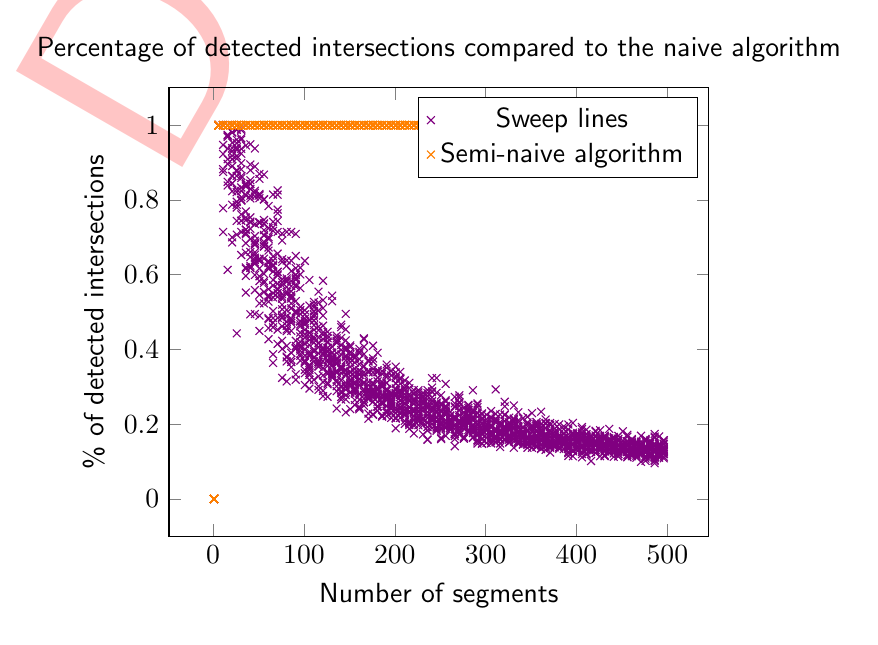
\begin{tikzpicture}
\begin{axis}[
    title={ Percentage of detected intersections compared to the naive algorithm},
    xlabel={ Number of segments },
    ylabel={ \% of detected intersections }
]

            \addplot[only marks, mark=x, color=violet] coordinates {
            (1, 0)
(1, 0)
(1, 0)
(1, 0)
(1, 0)
(1, 0)
(1, 0)
(1, 0)
(1, 0)
(1, 0)
(1, 0)
(1, 0)
(1, 0)
(1, 0)
(1, 0)
(1, 0)
(1, 0)
(1, 0)
(1, 0)
(1, 0)
(6, 1.0)
(6, 1.0)
(6, 1.0)
(6, 1.0)
(6, 1.0)
(6, 1.0)
(6, 1.0)
(6, 1.0)
(6, 1.0)
(6, 1.0)
(6, 1.0)
(6, 1.0)
(6, 1.0)
(6, 1.0)
(6, 1.0)
(6, 1.0)
(6, 1.0)
(6, 1.0)
(6, 1.0)
(6, 1.0)
(11, 0.7777777777777778)
(11, 1.0)
(11, 1.0)
(11, 1.0)
(11, 1.0)
(11, 0.9230769230769231)
(11, 1.0)
(11, 0.7142857142857143)
(11, 1.0)
(11, 1.0)
(11, 0.875)
(11, 0.9473684210526315)
(11, 0.8823529411764706)
(11, 1.0)
(11, 1.0)
(11, 1.0)
(11, 1.0)
(11, 1.0)
(11, 1.0)
(11, 1.0)
(16, 1.0)
(16, 1.0)
(16, 1.0)
(16, 1.0)
(16, 0.8387096774193549)
(16, 0.896551724137931)
(16, 0.9375)
(16, 0.9090909090909091)
(16, 1.0)
(16, 1.0)
(16, 1.0)
(16, 1.0)
(16, 1.0)
(16, 1.0)
(16, 0.6129032258064516)
(16, 1.0)
(16, 0.9722222222222222)
(16, 0.96875)
(16, 0.9743589743589743)
(16, 0.8484848484848485)
(21, 1.0)
(21, 0.8235294117647058)
(21, 0.8444444444444444)
(21, 1.0)
(21, 1.0)
(21, 0.8444444444444444)
(21, 0.890625)
(21, 0.9814814814814815)
(21, 0.7872340425531915)
(21, 0.9387755102040817)
(21, 0.8648648648648649)
(21, 0.7)
(21, 0.8636363636363636)
(21, 0.6862745098039216)
(21, 0.9090909090909091)
(21, 0.9183673469387755)
(21, 0.9534883720930233)
(21, 0.9803921568627451)
(21, 0.9305555555555556)
(21, 1.0)
(26, 0.7070707070707071)
(26, 0.8208955223880597)
(26, 0.7439024390243902)
(26, 0.88)
(26, 0.9876543209876543)
(26, 0.9344262295081968)
(26, 0.9880952380952381)
(26, 0.8767123287671232)
(26, 0.7951807228915663)
(26, 0.9354838709677419)
(26, 0.44285714285714284)
(26, 0.9523809523809523)
(26, 0.9615384615384616)
(26, 0.7796610169491526)
(26, 0.8641975308641975)
(26, 0.7866666666666666)
(26, 0.9405940594059405)
(26, 0.9176470588235294)
(26, 0.9104477611940298)
(26, 0.828125)
(31, 0.7980769230769231)
(31, 0.8071428571428572)
(31, 0.9907407407407407)
(31, 0.8)
(31, 0.8333333333333334)
(31, 0.8985507246376812)
(31, 0.9655172413793104)
(31, 0.9868421052631579)
(31, 0.7443609022556391)
(31, 0.9239130434782609)
(31, 0.9367088607594937)
(31, 0.9615384615384616)
(31, 0.8584070796460177)
(31, 0.8817204301075269)
(31, 0.8640776699029126)
(31, 0.652542372881356)
(31, 0.7142857142857143)
(31, 0.7613636363636364)
(31, 0.8243243243243243)
(31, 0.8)
(36, 0.7207792207792207)
(36, 0.6842105263157895)
(36, 0.8391608391608392)
(36, 0.8431372549019608)
(36, 0.8428571428571429)
(36, 0.7530120481927711)
(36, 0.7077922077922078)
(36, 0.7117117117117117)
(36, 0.8125)
(36, 0.7692307692307693)
(36, 0.5966850828729282)
(36, 0.8360655737704918)
(36, 0.5521472392638037)
(36, 0.8137254901960784)
(36, 0.72)
(36, 0.7457627118644068)
(36, 0.9458128078817734)
(36, 0.6160714285714286)
(36, 0.6194690265486725)
(36, 0.6590909090909091)
(41, 0.8289473684210527)
(41, 0.8950617283950617)
(41, 0.6473029045643154)
(41, 0.8525641025641025)
(41, 0.7398843930635838)
(41, 0.8435754189944135)
(41, 0.7532467532467533)
(41, 0.6181818181818182)
(41, 0.7230046948356808)
(41, 0.8113207547169812)
(41, 0.4939759036144578)
(41, 0.803921568627451)
(41, 0.6238532110091743)
(41, 0.6954314720812182)
(41, 0.7425149700598802)
(41, 0.6608695652173913)
(41, 0.8425925925925926)
(41, 0.6190476190476191)
(41, 0.9489795918367347)
(41, 0.8795180722891566)
(46, 0.7353951890034365)
(46, 0.809322033898305)
(46, 0.599290780141844)
(46, 0.6535433070866141)
(46, 0.49480968858131485)
(46, 0.6815286624203821)
(46, 0.659919028340081)
(46, 0.8894472361809045)
(46, 0.6454183266932271)
(46, 0.6851851851851852)
(46, 0.6394052044609665)
(46, 0.6797153024911032)
(46, 0.8246268656716418)
(46, 0.6907216494845361)
(46, 0.7032520325203252)
(46, 0.6291666666666667)
(46, 0.6331168831168831)
(46, 0.9377289377289377)
(46, 0.5586854460093896)
(46, 0.8191489361702128)
(51, 0.6417445482866043)
(51, 0.7408759124087592)
(51, 0.8565022421524664)
(51, 0.8048780487804879)
(51, 0.5955882352941176)
(51, 0.8125)
(51, 0.5828571428571429)
(51, 0.545751633986928)
(51, 0.6394052044609665)
(51, 0.6426332288401254)
(51, 0.8697478991596639)
(51, 0.4493927125506073)
(51, 0.7388059701492538)
(51, 0.811965811965812)
(51, 0.636604774535809)
(51, 0.4904214559386973)
(51, 0.7386363636363636)
(51, 0.5231788079470199)
(51, 0.8160377358490566)
(51, 0.6166134185303515)
(56, 0.6756756756756757)
(56, 0.8011869436201781)
(56, 0.6763848396501457)
(56, 0.7044198895027625)
(56, 0.7351351351351352)
(56, 0.6820512820512821)
(56, 0.5231316725978647)
(56, 0.7371601208459214)
(56, 0.7063953488372093)
(56, 0.6875)
(56, 0.7462121212121212)
(56, 0.8678756476683938)
(56, 0.6754098360655738)
(56, 0.5828571428571429)
(56, 0.7192982456140351)
(56, 0.6428571428571429)
(56, 0.8020833333333334)
(56, 0.5782122905027933)
(56, 0.5536159600997507)
(56, 0.6023738872403561)
(61, 0.7003154574132492)
(61, 0.6363636363636364)
(61, 0.5422885572139303)
(61, 0.7837259100642399)
(61, 0.5445783132530121)
(61, 0.4838709677419355)
(61, 0.6215384615384615)
(61, 0.6172248803827751)
(61, 0.6319444444444444)
(61, 0.5612745098039216)
(61, 0.5393518518518519)
(61, 0.5279850746268657)
(61, 0.664367816091954)
(61, 0.6728110599078341)
(61, 0.4802065404475043)
(61, 0.42718446601941745)
(61, 0.6159600997506235)
(61, 0.7242888402625821)
(61, 0.4570230607966457)
(61, 0.6955380577427821)
(66, 0.7174515235457064)
(66, 0.6490486257928119)
(66, 0.5504273504273505)
(66, 0.6374407582938388)
(66, 0.814498933901919)
(66, 0.608286252354049)
(66, 0.47155963302752296)
(66, 0.6224719101123596)
(66, 0.539179104477612)
(66, 0.7268408551068883)
(66, 0.5025380710659898)
(66, 0.7414187643020596)
(66, 0.5711297071129707)
(66, 0.6244444444444445)
(66, 0.45918367346938777)
(66, 0.6264367816091954)
(66, 0.36394557823129253)
(66, 0.48377125193199383)
(66, 0.3867768595041322)
(66, 0.5859519408502772)
(71, 0.48451730418943534)
(71, 0.6563636363636364)
(71, 0.5620214395099541)
(71, 0.5978128797083839)
(71, 0.41467576791808874)
(71, 0.7436762225969646)
(71, 0.7741433021806854)
(71, 0.5595026642984015)
(71, 0.8255813953488372)
(71, 0.6079447322970639)
(71, 0.6073394495412844)
(71, 0.7643884892086331)
(71, 0.7142857142857143)
(71, 0.6006768189509306)
(71, 0.5506535947712419)
(71, 0.8141592920353983)
(71, 0.5406203840472673)
(71, 0.5620805369127517)
(71, 0.5756385068762279)
(71, 0.4528301886792453)
(76, 0.5716292134831461)
(76, 0.5874524714828897)
(76, 0.4867021276595745)
(76, 0.5794223826714802)
(76, 0.4926052332195677)
(76, 0.5477815699658704)
(76, 0.6916167664670658)
(76, 0.4230769230769231)
(76, 0.5196211096075778)
(76, 0.6341789052069426)
(76, 0.5072254335260116)
(76, 0.4838709677419355)
(76, 0.46168958742632615)
(76, 0.4852459016393443)
(76, 0.5409356725146199)
(76, 0.7100313479623824)
(76, 0.6415384615384615)
(76, 0.32386363636363635)
(76, 0.4013333333333333)
(76, 0.5353846153846153)
(81, 0.590027700831025)
(81, 0.6380697050938338)
(81, 0.7144808743169399)
(81, 0.4093655589123867)
(81, 0.5812417437252312)
(81, 0.548480463096961)
(81, 0.3783068783068783)
(81, 0.5540679711637487)
(81, 0.3143712574850299)
(81, 0.45342706502636204)
(81, 0.38070404172099087)
(81, 0.3677581863979849)
(81, 0.5847222222222223)
(81, 0.4489051094890511)
(81, 0.6239316239316239)
(81, 0.46320346320346323)
(81, 0.47389033942558745)
(81, 0.48847926267281105)
(81, 0.5053908355795148)
(81, 0.5670241286863271)
(86, 0.5233545647558386)
(86, 0.3662420382165605)
(86, 0.5398230088495575)
(86, 0.714614499424626)
(86, 0.3527054108216433)
(86, 0.5101156069364162)
(86, 0.4811800610376399)
(86, 0.476409666283084)
(86, 0.3726190476190476)
(86, 0.5362663495838288)
(86, 0.5833333333333334)
(86, 0.4831981460023175)
(86, 0.6096345514950167)
(86, 0.44960362400906)
(86, 0.6375838926174496)
(86, 0.544924154025671)
(86, 0.5555555555555556)
(86, 0.5691964285714286)
(86, 0.47129909365558914)
(86, 0.3909677419354839)
(91, 0.5292712066905615)
(91, 0.6172839506172839)
(91, 0.31864754098360654)
(91, 0.4016393442622951)
(91, 0.573404255319149)
(91, 0.5682859761686526)
(91, 0.5026737967914439)
(91, 0.49686192468619245)
(91, 0.6002358490566038)
(91, 0.40919037199124725)
(91, 0.7091469681397738)
(91, 0.5879781420765028)
(91, 0.49888641425389757)
(91, 0.591991341991342)
(91, 0.3329969727547931)
(91, 0.586489252814739)
(91, 0.4230038022813688)
(91, 0.650049850448654)
(91, 0.598989898989899)
(91, 0.40423572744014735)
(96, 0.3827450980392157)
(96, 0.5137362637362637)
(96, 0.4949186991869919)
(96, 0.6006674082313682)
(96, 0.40714285714285714)
(96, 0.5640096618357487)
(96, 0.38841567291311757)
(96, 0.4450610432852386)
(96, 0.3966850828729282)
(96, 0.47550866616428034)
(96, 0.4120287253141831)
(96, 0.43462017434620176)
(96, 0.61875)
(96, 0.504950495049505)
(96, 0.4616805170821791)
(96, 0.3697967086156825)
(96, 0.4200595829195631)
(96, 0.47433460076045625)
(96, 0.46722846441947563)
(96, 0.40487804878048783)
(101, 0.40053763440860213)
(101, 0.3694690265486726)
(101, 0.3045886075949367)
(101, 0.47070124879923153)
(101, 0.33634719710669075)
(101, 0.47525597269624575)
(101, 0.3836363636363636)
(101, 0.49370277078085645)
(101, 0.636899747262005)
(101, 0.4662638469284995)
(101, 0.36459246275197194)
(101, 0.3663440059568131)
(101, 0.3451008645533141)
(101, 0.5048471290082028)
(101, 0.45216606498194944)
(101, 0.43186003683241253)
(101, 0.48221343873517786)
(101, 0.41588385994876176)
(101, 0.4403361344537815)
(101, 0.41423948220064727)
(106, 0.4117647058823529)
(106, 0.3934540389972145)
(106, 0.477891156462585)
(106, 0.3498452012383901)
(106, 0.3541666666666667)
(106, 0.3375277572168764)
(106, 0.38270616493194554)
(106, 0.3866782006920415)
(106, 0.2951219512195122)
(106, 0.4435336976320583)
(106, 0.4248985115020298)
(106, 0.47952684258416745)
(106, 0.35860655737704916)
(106, 0.44537815126050423)
(106, 0.5173192771084337)
(106, 0.43433544303797467)
(106, 0.3448047650562541)
(106, 0.33134684147794996)
(106, 0.5856741573033708)
(106, 0.3182827535159141)
(111, 0.37905405405405407)
(111, 0.45230369889682026)
(111, 0.5013458950201884)
(111, 0.4871987951807229)
(111, 0.31862745098039214)
(111, 0.4331306990881459)
(111, 0.39902971497877504)
(111, 0.42749371332774516)
(111, 0.47730829420970267)
(111, 0.41794871794871796)
(111, 0.5025792188651437)
(111, 0.5129449838187702)
(111, 0.3680232558139535)
(111, 0.4774247491638796)
(111, 0.5271428571428571)
(111, 0.46504369538077406)
(111, 0.5193409742120344)
(111, 0.49333333333333335)
(111, 0.39398385913426265)
(111, 0.37735849056603776)
(116, 0.4319488817891374)
(116, 0.5040431266846361)
(116, 0.30097087378640774)
(116, 0.418049104180491)
(116, 0.5546528803545052)
(116, 0.46102819237147596)
(116, 0.40577617328519855)
(116, 0.29159978598180847)
(116, 0.3663522012578616)
(116, 0.4160861304623179)
(116, 0.5252043596730245)
(116, 0.37178642056690836)
(116, 0.45163240628778717)
(116, 0.36698808848553605)
(116, 0.35426356589147284)
(116, 0.3894348894348894)
(116, 0.36097560975609755)
(116, 0.35477318889641163)
(116, 0.3279181708784597)
(116, 0.3653741125068269)
(121, 0.2891770011273957)
(121, 0.33060556464811786)
(121, 0.39798206278026904)
(121, 0.4040284360189573)
(121, 0.3997827267789245)
(121, 0.4453973699256718)
(121, 0.39947780678851175)
(121, 0.5317829457364341)
(121, 0.5836807623585467)
(121, 0.5105028644175684)
(121, 0.38633461047254153)
(121, 0.4904996481351161)
(121, 0.42724252491694353)
(121, 0.27496236828901155)
(121, 0.38999358563181524)
(121, 0.4390084801043705)
(121, 0.3124673969744392)
(121, 0.3497989661114302)
(121, 0.4633587786259542)
(121, 0.3687150837988827)
(126, 0.27307904919845216)
(126, 0.4298300818124607)
(126, 0.40413997042878264)
(126, 0.36598209583991576)
(126, 0.37162519851773423)
(126, 0.3970080552359033)
(126, 0.30648899188876016)
(126, 0.4181913225300575)
(126, 0.3718510405257393)
(126, 0.355775169857937)
(126, 0.40415584415584416)
(126, 0.43659621802002224)
(126, 0.3403890160183066)
(126, 0.38221153846153844)
(126, 0.3346153846153846)
(126, 0.3929554210236654)
(126, 0.4210829493087558)
(126, 0.44704433497536944)
(126, 0.3105590062111801)
(126, 0.3843843843843844)
(131, 0.37073170731707317)
(131, 0.40716612377850164)
(131, 0.39145496535796764)
(131, 0.3604385564184559)
(131, 0.36718332442544094)
(131, 0.37524177949709864)
(131, 0.37277486910994767)
(131, 0.3245067497403946)
(131, 0.3331850533807829)
(131, 0.33423180592991913)
(131, 0.3559822747415066)
(131, 0.37389597644749756)
(131, 0.3285135916714864)
(131, 0.33590361445783135)
(131, 0.3809749171793658)
(131, 0.38998682476943347)
(131, 0.5437605872388481)
(131, 0.37410805300713557)
(131, 0.5288915094339622)
(131, 0.34063526834611174)
(136, 0.417458432304038)
(136, 0.42934782608695654)
(136, 0.3128916741271262)
(136, 0.2882439744220364)
(136, 0.3418217433888345)
(136, 0.3384180790960452)
(136, 0.4188073394495413)
(136, 0.3902932254802831)
(136, 0.33778801843317974)
(136, 0.4229713837710702)
(136, 0.3712494402149575)
(136, 0.24172661870503598)
(136, 0.3759505703422053)
(136, 0.4368421052631579)
(136, 0.37537993920972645)
(136, 0.30122591943957966)
(136, 0.36527215474583896)
(136, 0.36127744510978044)
(136, 0.31745283018867926)
(136, 0.36305048335123524)
(141, 0.30230326295585414)
(141, 0.2987747408105561)
(141, 0.4595103578154426)
(141, 0.39853826311263973)
(141, 0.3861788617886179)
(141, 0.3363006923837784)
(141, 0.3548672566371681)
(141, 0.26580350342726583)
(141, 0.2725274725274725)
(141, 0.34823848238482386)
(141, 0.2877221992558909)
(141, 0.2835563228312473)
(141, 0.31734960767218834)
(141, 0.41158267020335987)
(141, 0.43093093093093093)
(141, 0.3473127035830619)
(141, 0.3508847647820457)
(141, 0.35270629991126884)
(141, 0.46628969117007396)
(141, 0.3462246777163904)
(146, 0.2922242314647378)
(146, 0.398061613014884)
(146, 0.38303233935321296)
(146, 0.333835719668425)
(146, 0.3310120705663881)
(146, 0.4021551724137931)
(146, 0.34319787985865724)
(146, 0.4533446953557733)
(146, 0.2998411437648928)
(146, 0.303662859393462)
(146, 0.2663677130044843)
(146, 0.3110454377539712)
(146, 0.3459422283356259)
(146, 0.2774888558692422)
(146, 0.3703547297297297)
(146, 0.4060751398880895)
(146, 0.37902483900643974)
(146, 0.4238975817923186)
(146, 0.23139617292700213)
(146, 0.49503311258278143)
(151, 0.39288417865253594)
(151, 0.2849162011173184)
(151, 0.3191489361702128)
(151, 0.3062330623306233)
(151, 0.30853563038371185)
(151, 0.38625678119349005)
(151, 0.28457927049476345)
(151, 0.3657650383528462)
(151, 0.3009353395689305)
(151, 0.3286908077994429)
(151, 0.4063173007896626)
(151, 0.33833063209076175)
(151, 0.31414868105515587)
(151, 0.34011627906976744)
(151, 0.4107008289374529)
(151, 0.3755274261603376)
(151, 0.3532818532818533)
(151, 0.37453950061399915)
(151, 0.3401301518438178)
(151, 0.24011502516175415)
(156, 0.3278301886792453)
(156, 0.3384446878422782)
(156, 0.38536060279870826)
(156, 0.2867048537835393)
(156, 0.37966101694915255)
(156, 0.29401767505098575)
(156, 0.2936901222332342)
(156, 0.3767409470752089)
(156, 0.3482604202549087)
(156, 0.3085770621097601)
(156, 0.2644694533762058)
(156, 0.29023288147375736)
(156, 0.3645955451348183)
(156, 0.31241997439180536)
(156, 0.3278972935461485)
(156, 0.2510500807754443)
(156, 0.28174737555028784)
(156, 0.30710113741162004)
(156, 0.2972549019607843)
(156, 0.3285891089108911)
(161, 0.38978054372748117)
(161, 0.3936894944424525)
(161, 0.33205974296630775)
(161, 0.3734083506070477)
(161, 0.3215356928614277)
(161, 0.24588511924756465)
(161, 0.2652931854199683)
(161, 0.3436935308998916)
(161, 0.31929696082021236)
(161, 0.28095238095238095)
(161, 0.335061088485746)
(161, 0.3059418457648546)
(161, 0.3040054775761725)
(161, 0.3128858024691358)
(161, 0.343522056269538)
(161, 0.4017605633802817)
(161, 0.2396486825595985)
(161, 0.24342105263157895)
(161, 0.3600649350649351)
(161, 0.33191747572815533)
(166, 0.35438098616530683)
(166, 0.42974944497304157)
(166, 0.2926605504587156)
(166, 0.25823045267489714)
(166, 0.27767584097859327)
(166, 0.31197183098591547)
(166, 0.2488306828811974)
(166, 0.2861337683523654)
(166, 0.2912004838221953)
(166, 0.42695652173913046)
(166, 0.4067850348763475)
(166, 0.2578879587894398)
(166, 0.38715338715338715)
(166, 0.25894948143191704)
(166, 0.3317729666471621)
(166, 0.26793431287813313)
(166, 0.35563858695652173)
(166, 0.31044303797468353)
(166, 0.3386180077774454)
(166, 0.30871705763104546)
(171, 0.2667377967457989)
(171, 0.288778364936276)
(171, 0.2737682165163081)
(171, 0.3709501274117219)
(171, 0.22827282728272827)
(171, 0.3385004745333755)
(171, 0.2799174690508941)
(171, 0.2936880542514345)
(171, 0.31294559099437147)
(171, 0.29269647320188835)
(171, 0.2901915264074289)
(171, 0.27474972191323693)
(171, 0.28507126781695424)
(171, 0.3043189368770764)
(171, 0.267853170189099)
(171, 0.21449792038027332)
(171, 0.3676738259919913)
(171, 0.26920995670995673)
(171, 0.33874778499704666)
(171, 0.3427538613210647)
(176, 0.3383084577114428)
(176, 0.3676430331234602)
(176, 0.2716352716352716)
(176, 0.3471307619943556)
(176, 0.40972008612734545)
(176, 0.28609341825902335)
(176, 0.2804517343371874)
(176, 0.30677607199576495)
(176, 0.2911914583838874)
(176, 0.28575547866205303)
(176, 0.22501365374112506)
(176, 0.375743162901308)
(176, 0.31057401812688823)
(176, 0.28360215053763443)
(176, 0.27676313571227873)
(176, 0.2264540891644523)
(176, 0.2936926924145596)
(176, 0.29191797346200243)
(176, 0.27845420857596614)
(176, 0.25979714153988015)
(181, 0.29037850332273907)
(181, 0.2819961795606495)
(181, 0.3398868839213574)
(181, 0.29746254967899727)
(181, 0.29394729220967275)
(181, 0.24802110817941952)
(181, 0.3244217482727546)
(181, 0.25970686551812805)
(181, 0.3407243163340724)
(181, 0.24768902583550603)
(181, 0.34454230050707235)
(181, 0.39102932719954)
(181, 0.31461001164144353)
(181, 0.2771016133597509)
(181, 0.27303657499291184)
(181, 0.23589615576635048)
(181, 0.2800207039337474)
(181, 0.2738610333418173)
(181, 0.3384279475982533)
(181, 0.24563233376792698)
(186, 0.27694782808549756)
(186, 0.25413078892250407)
(186, 0.3417631765540061)
(186, 0.2586165341046035)
(186, 0.3131338742393509)
(186, 0.3343480466768138)
(186, 0.25493421052631576)
(186, 0.30837961844964984)
(186, 0.25921787709497207)
(186, 0.26976495726495725)
(186, 0.30155544405418966)
(186, 0.30450267107606205)
(186, 0.2226492441711504)
(186, 0.3012992369560734)
(186, 0.22315348349921424)
(186, 0.2992565055762082)
(186, 0.30021197668256494)
(186, 0.2696825793551612)
(186, 0.27739481816020917)
(186, 0.21971985718209283)
(191, 0.22182920667003536)
(191, 0.35085513078470826)
(191, 0.27192297684100963)
(191, 0.2488)
(191, 0.3105513111707619)
(191, 0.2941793392763503)
(191, 0.26881720430107525)
(191, 0.23478444632290787)
(191, 0.26385707741639947)
(191, 0.2895927601809955)
(191, 0.309631985461154)
(191, 0.2782031648800408)
(191, 0.28977006100422337)
(191, 0.23644158628081458)
(191, 0.3261291216403436)
(191, 0.23032936870997256)
(191, 0.3325266214908035)
(191, 0.2818838890184192)
(191, 0.35944577671196376)
(191, 0.27308312226571496)
(196, 0.24222369291859697)
(196, 0.23060483009189997)
(196, 0.2403846153846154)
(196, 0.27803480942938974)
(196, 0.2786885245901639)
(196, 0.2831050228310502)
(196, 0.2669872464980138)
(196, 0.24687962767082716)
(196, 0.2166830225711482)
(196, 0.33028545941124)
(196, 0.3426978818283166)
(196, 0.25370641052411774)
(196, 0.2655730897009967)
(196, 0.27373312679796413)
(196, 0.28062678062678065)
(196, 0.28291694800810263)
(196, 0.2581492014876395)
(196, 0.2620704654197477)
(196, 0.2552362396492937)
(196, 0.24796837250164727)
(201, 0.23744104982571254)
(201, 0.3082778306374881)
(201, 0.1888551604509974)
(201, 0.2438555246847617)
(201, 0.21743161798794622)
(201, 0.2783438109690006)
(201, 0.2756585879873551)
(201, 0.23027143627539098)
(201, 0.21558743699108182)
(201, 0.2834467120181406)
(201, 0.3097236438075742)
(201, 0.29187761391151223)
(201, 0.32310934207445563)
(201, 0.328589634664401)
(201, 0.2813594954449895)
(201, 0.27882817369623936)
(201, 0.29555108428347865)
(201, 0.3383233532934132)
(201, 0.2150428047289034)
(201, 0.35394226626454117)
(206, 0.30852211434735705)
(206, 0.2315270935960591)
(206, 0.2645631067961165)
(206, 0.2804611409262572)
(206, 0.3201647631529676)
(206, 0.21652421652421652)
(206, 0.2864478678276401)
(206, 0.2903014416775885)
(206, 0.24633699633699635)
(206, 0.2782998718496369)
(206, 0.26221357544314744)
(206, 0.32396166134185306)
(206, 0.2404263718910383)
(206, 0.3397862472272636)
(206, 0.24568337840649054)
(206, 0.2727634194831014)
(206, 0.27929498353670346)
(206, 0.2273449920508744)
(206, 0.2907002429865253)
(206, 0.25361834780672454)
(211, 0.2004885993485342)
(211, 0.2963951935914553)
(211, 0.22682009294091612)
(211, 0.2808300395256917)
(211, 0.2574754622232367)
(211, 0.2541216600341103)
(211, 0.2302560403894699)
(211, 0.22413070800167575)
(211, 0.20862396956246038)
(211, 0.29050925925925924)
(211, 0.22370617696160267)
(211, 0.30362972921067793)
(211, 0.2461638210503566)
(211, 0.27311129163281883)
(211, 0.23042783596662525)
(211, 0.23947215214438192)
(211, 0.31689119170984453)
(211, 0.26600221483942416)
(211, 0.22809387134897857)
(211, 0.23661429945495352)
(216, 0.2619911326078194)
(216, 0.2450057784381707)
(216, 0.23410355877888345)
(216, 0.1873938478958294)
(216, 0.20138339920948617)
(216, 0.1974388379204893)
(216, 0.26665422653480125)
(216, 0.2346348517715112)
(216, 0.2642211589580011)
(216, 0.24439024390243902)
(216, 0.2294936988724298)
(216, 0.2961279767315034)
(216, 0.2041124316166761)
(216, 0.2791386803634927)
(216, 0.2736105713175282)
(216, 0.2791645440652063)
(216, 0.20679886685552407)
(216, 0.24477135767458347)
(216, 0.20294275973443388)
(216, 0.31037753746917096)
(221, 0.29140160065667964)
(221, 0.280602978568834)
(221, 0.21031949427643942)
(221, 0.220890129742158)
(221, 0.22095671981776766)
(221, 0.23422263109475622)
(221, 0.23869296672643953)
(221, 0.21256378673235968)
(221, 0.2546119039331709)
(221, 0.2612309519097566)
(221, 0.23914670658682635)
(221, 0.19549464398235664)
(221, 0.25424361126655476)
(221, 0.23286354900704676)
(221, 0.26246918262848473)
(221, 0.17506889285135355)
(221, 0.2823014804845222)
(221, 0.2673434856175973)
(221, 0.2667748917748918)
(221, 0.20018691588785048)
(226, 0.25257025359835505)
(226, 0.2195210449927431)
(226, 0.2434119278779473)
(226, 0.2335994989823078)
(226, 0.26986831913245546)
(226, 0.21517085993240706)
(226, 0.2850805126519882)
(226, 0.23196881091617932)
(226, 0.2520023442078531)
(226, 0.21352371573937304)
(226, 0.23307510946446616)
(226, 0.21160580290145073)
(226, 0.23426946320654107)
(226, 0.29083067691730735)
(226, 0.1969104783175135)
(226, 0.20703585255007576)
(226, 0.2786532951289398)
(226, 0.2251678430022379)
(226, 0.23619894035207656)
(226, 0.2604130808950086)
(231, 0.28348288467929544)
(231, 0.2608624632473048)
(231, 0.21547054840893703)
(231, 0.20411985018726592)
(231, 0.2417785234899329)
(231, 0.2447814451382694)
(231, 0.2536115569823435)
(231, 0.27059218251971145)
(231, 0.27639751552795033)
(231, 0.21674114816088003)
(231, 0.2130407718643013)
(231, 0.25566884796834577)
(231, 0.2127371273712737)
(231, 0.19705617302493242)
(231, 0.26260812795821775)
(231, 0.2610052562417871)
(231, 0.17249490355966757)
(231, 0.21272727272727274)
(231, 0.26310060643756805)
(231, 0.23462516833757294)
(236, 0.2826794586260065)
(236, 0.2463745516918759)
(236, 0.2756349952963311)
(236, 0.2748640589370286)
(236, 0.15901568571017413)
(236, 0.182925122463261)
(236, 0.2233128834355828)
(236, 0.266162310866575)
(236, 0.24219369155175147)
(236, 0.20342543221845208)
(236, 0.21663604476365458)
(236, 0.24934261407579272)
(236, 0.2321628988295655)
(236, 0.19222430987136868)
(236, 0.223628024671833)
(236, 0.15783227848101267)
(236, 0.2247557003257329)
(236, 0.20431866513986585)
(236, 0.29096264145093786)
(236, 0.2552418689120026)
(241, 0.21412437885860564)
(241, 0.2186816192560175)
(241, 0.25413416536661465)
(241, 0.22142857142857142)
(241, 0.26140432819554726)
(241, 0.23688634835238737)
(241, 0.29792392786785876)
(241, 0.2120939979045053)
(241, 0.24619026483207576)
(241, 0.21336007405121876)
(241, 0.2712130735386549)
(241, 0.20862755167543973)
(241, 0.2877281495770886)
(241, 0.23378076062639822)
(241, 0.3230378991345867)
(241, 0.1893027163259591)
(241, 0.20083413538658967)
(241, 0.28531976744186044)
(241, 0.21666095303393898)
(241, 0.24222153080273803)
(246, 0.21852266368214884)
(246, 0.23044054810667453)
(246, 0.2083223249669749)
(246, 0.20721105885706143)
(246, 0.23604158644589912)
(246, 0.24870848708487084)
(246, 0.2837070678399092)
(246, 0.2559797949784579)
(246, 0.32340425531914896)
(246, 0.18202416918429004)
(246, 0.24180616120410747)
(246, 0.2165503199534613)
(246, 0.2345513963161022)
(246, 0.2525097601784718)
(246, 0.1857196168677696)
(246, 0.19156626506024096)
(246, 0.19055745164960183)
(246, 0.20629470672389127)
(246, 0.21783507923717432)
(246, 0.2576846612631901)
(251, 0.27725148414803585)
(251, 0.2364112639161755)
(251, 0.20409468969929623)
(251, 0.25523232855074374)
(251, 0.19950287807430664)
(251, 0.21721994846142187)
(251, 0.2216897165548405)
(251, 0.20501232539030403)
(251, 0.23307900566084175)
(251, 0.22124137931034482)
(251, 0.25142606406318563)
(251, 0.15989533122159483)
(251, 0.19789445628997868)
(251, 0.23445109224989563)
(251, 0.16354808147797253)
(251, 0.2124321946928603)
(251, 0.18579899650296489)
(251, 0.19019208381839348)
(251, 0.1895324494068388)
(251, 0.21832167832167831)
(256, 0.20345084409136047)
(256, 0.19407982855612108)
(256, 0.16864931846344486)
(256, 0.24581450969970767)
(256, 0.2603658536585366)
(256, 0.2637484416124117)
(256, 0.23673469387755103)
(256, 0.233594060718547)
(256, 0.24854969704782776)
(256, 0.20303657694962043)
(256, 0.22493189778181347)
(256, 0.23200889135871075)
(256, 0.20090634441087613)
(256, 0.1894722885176346)
(256, 0.23197087150575524)
(256, 0.22958418541240627)
(256, 0.2471492017764974)
(256, 0.24209661967975912)
(256, 0.20986850670485613)
(256, 0.307557826788596)
(261, 0.19745385105028646)
(261, 0.21338752699098185)
(261, 0.19583388616160277)
(261, 0.2030806647750304)
(261, 0.20363761943133418)
(261, 0.18531949481055396)
(261, 0.21181746241097335)
(261, 0.23201856148491878)
(261, 0.18526142445450802)
(261, 0.18984771573604062)
(261, 0.20671931803936316)
(261, 0.19702475584828527)
(261, 0.21257665023445954)
(261, 0.2083445130131473)
(261, 0.20083374203040708)
(261, 0.21205673758865248)
(261, 0.22141662018962632)
(261, 0.20905967680366458)
(261, 0.1913992297817715)
(261, 0.2230347349177331)
(266, 0.2126960963152134)
(266, 0.24758594051757435)
(266, 0.1939204613721014)
(266, 0.14081237911025146)
(266, 0.22011072871464912)
(266, 0.17385316241127238)
(266, 0.1680594243268338)
(266, 0.21327919751612132)
(266, 0.21696658097686375)
(266, 0.15970921907699087)
(266, 0.2152963671128107)
(266, 0.25563648976760317)
(266, 0.273059138476515)
(266, 0.17277848028509024)
(266, 0.2455310199789695)
(266, 0.19824996735013714)
(266, 0.2194859372897322)
(266, 0.1867398044359647)
(266, 0.17494824016563146)
(266, 0.21120058565153735)
(271, 0.17345132743362832)
(271, 0.25908543922984356)
(271, 0.277148253068933)
(271, 0.19272021907804657)
(271, 0.23816517907581064)
(271, 0.2559760956175299)
(271, 0.21038477451386015)
(271, 0.17268247966082273)
(271, 0.20611427878199684)
(271, 0.22401847575057737)
(271, 0.20020651675080312)
(271, 0.20537897310513448)
(271, 0.24829208198006494)
(271, 0.20183372568454963)
(271, 0.23672674135411592)
(271, 0.27071465561885033)
(271, 0.17928332757230095)
(271, 0.20197975753531308)
(271, 0.1902954087080318)
(271, 0.18388903028760498)
(276, 0.20788058390955988)
(276, 0.22312323381250768)
(276, 0.1938208490775728)
(276, 0.231661511268228)
(276, 0.20082063305978898)
(276, 0.16106579662860251)
(276, 0.20767350409182697)
(276, 0.21732954545454544)
(276, 0.19818961410195332)
(276, 0.20185342991052407)
(276, 0.20936266215454033)
(276, 0.21140819964349375)
(276, 0.19628121905600177)
(276, 0.16134976390648392)
(276, 0.24319283849309958)
(276, 0.20334728033472804)
(276, 0.18708342909675937)
(276, 0.16563960900977476)
(276, 0.23126362906002526)
(276, 0.2021985343104597)
(281, 0.21917956488797488)
(281, 0.2102105377986255)
(281, 0.23747252747252748)
(281, 0.2516114180478821)
(281, 0.18433670751198722)
(281, 0.21589713617767387)
(281, 0.17831978319783198)
(281, 0.21957728437233134)
(281, 0.20562480684042445)
(281, 0.20842502357749135)
(281, 0.2129727198220349)
(281, 0.20101931966338746)
(281, 0.23347381095725467)
(281, 0.22406145190955318)
(281, 0.24315941065691812)
(281, 0.22509776857602945)
(281, 0.23786893446723362)
(281, 0.17945544554455445)
(281, 0.2207589503463077)
(281, 0.24918032786885247)
(286, 0.165056648777579)
(286, 0.19382051021445268)
(286, 0.2304729295955489)
(286, 0.2096961261888193)
(286, 0.21941023613151056)
(286, 0.19781221513217867)
(286, 0.19686892458815103)
(286, 0.19693821760524877)
(286, 0.18471681798530049)
(286, 0.16292319491618276)
(286, 0.18882836697639646)
(286, 0.29065702230259194)
(286, 0.18085444715360968)
(286, 0.2142459654980523)
(286, 0.23680273562727078)
(286, 0.1967079861816704)
(286, 0.21383395241441622)
(286, 0.18474777991394306)
(286, 0.23480542195015303)
(286, 0.17608337904552934)
(291, 0.19078415521422798)
(291, 0.25544937184580696)
(291, 0.17099970568036887)
(291, 0.16915372035977105)
(291, 0.1480025499362516)
(291, 0.17817807514153372)
(291, 0.23094437818497235)
(291, 0.2192435577722361)
(291, 0.19787212886546685)
(291, 0.19976938599019892)
(291, 0.153587686971602)
(291, 0.1573871545038775)
(291, 0.252326565143824)
(291, 0.20143329658213893)
(291, 0.2289156626506024)
(291, 0.17242860210435904)
(291, 0.24555518282455552)
(291, 0.20025176721216228)
(291, 0.18538860103626942)
(291, 0.2073568371713878)
(296, 0.19306345968001717)
(296, 0.17210247150434488)
(296, 0.21250455041863853)
(296, 0.21549421193232413)
(296, 0.20255748979153235)
(296, 0.16095380029806258)
(296, 0.17665321328779882)
(296, 0.17483296213808464)
(296, 0.18532326998272255)
(296, 0.22877382021350892)
(296, 0.21519246519246518)
(296, 0.20260421727723255)
(296, 0.22610584518167456)
(296, 0.18474694242815948)
(296, 0.18504233301975542)
(296, 0.1833509972058965)
(296, 0.1593204775022957)
(296, 0.14836282285946714)
(296, 0.14694637780609743)
(296, 0.2016209614744088)
(301, 0.19781975378253924)
(301, 0.2067818534602236)
(301, 0.18572547483845703)
(301, 0.19049436915441878)
(301, 0.22541831171272797)
(301, 0.20020467020187924)
(301, 0.1884857281083696)
(301, 0.18267335602938542)
(301, 0.1869969040247678)
(301, 0.21247216035634744)
(301, 0.18832371201394182)
(301, 0.1876416245424438)
(301, 0.18396185522323363)
(301, 0.19390715667311412)
(301, 0.16406530319339793)
(301, 0.18553167839940718)
(301, 0.18657575489241124)
(301, 0.17260888129803587)
(301, 0.14974150664697194)
(301, 0.18876425156307466)
(306, 0.1773477720575182)
(306, 0.16763173132599885)
(306, 0.17411595763776702)
(306, 0.23485394879192212)
(306, 0.19158200290275762)
(306, 0.1916035656091249)
(306, 0.21862163395709722)
(306, 0.14968009371902316)
(306, 0.20750529607586)
(306, 0.17652538425710293)
(306, 0.15486402628216828)
(306, 0.1707671357240127)
(306, 0.16754930606281956)
(306, 0.21497305619707469)
(306, 0.1967098703888335)
(306, 0.2174554757453508)
(306, 0.17623974313235818)
(306, 0.18056589724497393)
(306, 0.1481346678798908)
(306, 0.15942728442728443)
(311, 0.20775569558894813)
(311, 0.18021260567506486)
(311, 0.15926167918980724)
(311, 0.29287190082644626)
(311, 0.16128764622915456)
(311, 0.22743006829450838)
(311, 0.15109913248547124)
(311, 0.1641407427102721)
(311, 0.16118603362276002)
(311, 0.20409522224071916)
(311, 0.1680783753444229)
(311, 0.16050775740479548)
(311, 0.16602155037137775)
(311, 0.15287711313394017)
(311, 0.18841911764705882)
(311, 0.2119696447050707)
(311, 0.18477640342530924)
(311, 0.16443752290216196)
(311, 0.21486093814860938)
(311, 0.17970537103120138)
(316, 0.1769822376854056)
(316, 0.17760727479397556)
(316, 0.1583410138248848)
(316, 0.1814757186143641)
(316, 0.19367941351297802)
(316, 0.16183391528768787)
(316, 0.1710964874797026)
(316, 0.1479211841236919)
(316, 0.1715272099572999)
(316, 0.1754581350612534)
(316, 0.19558517284464808)
(316, 0.20547677261613692)
(316, 0.17533512064343162)
(316, 0.20018388498829823)
(316, 0.18056120374135828)
(316, 0.20016222062004327)
(316, 0.13880847173548683)
(316, 0.16025641025641027)
(316, 0.22569234751099992)
(316, 0.183679354094579)
(321, 0.1566265060240964)
(321, 0.19226699226699226)
(321, 0.16015174006267524)
(321, 0.16005848456179583)
(321, 0.188706091596265)
(321, 0.19251766217084137)
(321, 0.1896866191344719)
(321, 0.17029635323255615)
(321, 0.18934854969091774)
(321, 0.2597300140252454)
(321, 0.18337850045167117)
(321, 0.17998882057015092)
(321, 0.2082906857727738)
(321, 0.1796698836475151)
(321, 0.223950233281493)
(321, 0.18825685149776927)
(321, 0.2257126705967859)
(321, 0.2475118996105582)
(321, 0.17284773731144262)
(321, 0.19396626673621978)
(326, 0.20424822990420657)
(326, 0.18643803585346844)
(326, 0.19057064388159903)
(326, 0.1863769327204346)
(326, 0.16747437832684517)
(326, 0.19230460921843687)
(326, 0.19462102689486552)
(326, 0.15079300528670192)
(326, 0.17205176202490438)
(326, 0.18914667715296893)
(326, 0.15864728090609687)
(326, 0.20353906650709522)
(326, 0.18404202922344443)
(326, 0.19749641806801901)
(326, 0.21729379516571143)
(326, 0.19719870222362904)
(326, 0.1523632844007098)
(326, 0.159134531495376)
(326, 0.1689239332096475)
(326, 0.16369257950530036)
(331, 0.16703609879670678)
(331, 0.24987093443469283)
(331, 0.21419966872458968)
(331, 0.16037329504666187)
(331, 0.18763548775592132)
(331, 0.13668478260869565)
(331, 0.15352136463435231)
(331, 0.18964813454159524)
(331, 0.16683333333333333)
(331, 0.20578728643989533)
(331, 0.21034220532319392)
(331, 0.15980119619240166)
(331, 0.1705683156654888)
(331, 0.21463937943555042)
(331, 0.17690721649484537)
(331, 0.17171888230313292)
(331, 0.1743845484049711)
(331, 0.1924721984602224)
(331, 0.19938247780779622)
(331, 0.17508302818700502)
(336, 0.1677657403046004)
(336, 0.15016151361329028)
(336, 0.14911746804625683)
(336, 0.15455674584691817)
(336, 0.1617125110913931)
(336, 0.15144517282479142)
(336, 0.19175597691673538)
(336, 0.19541800643086818)
(336, 0.18828622774056528)
(336, 0.16150271107668474)
(336, 0.2102980602428639)
(336, 0.1816526291827908)
(336, 0.15083333333333335)
(336, 0.2317269357207806)
(336, 0.20518810924031258)
(336, 0.1473644859813084)
(336, 0.1808693165570489)
(336, 0.17903006496449614)
(336, 0.1735110563217505)
(336, 0.181047197640118)
(341, 0.1906414985173935)
(341, 0.16848902913333821)
(341, 0.16249012709126157)
(341, 0.18016928657799275)
(341, 0.14664906877841324)
(341, 0.17804985986133648)
(341, 0.15347666971637694)
(341, 0.1636617749825297)
(341, 0.19126610116242537)
(341, 0.1784332688588008)
(341, 0.17340376665135507)
(341, 0.1644992014601871)
(341, 0.21540836373842268)
(341, 0.17811879676286457)
(341, 0.1756152972358955)
(341, 0.17388238612325482)
(341, 0.1802481148139139)
(341, 0.1714154712779197)
(341, 0.17506108615117838)
(341, 0.14502565564424175)
(346, 0.184322191617658)
(346, 0.14651126408010012)
(346, 0.1998085666427375)
(346, 0.1491829588561424)
(346, 0.1533246790711092)
(346, 0.2045585274662065)
(346, 0.19400759219088937)
(346, 0.14479205005520795)
(346, 0.21963470319634704)
(346, 0.1652821160364192)
(346, 0.18009621166566447)
(346, 0.15919903429666973)
(346, 0.14548301450064674)
(346, 0.1663619744058501)
(346, 0.1366579828805359)
(346, 0.16047460140897293)
(346, 0.18412103546394615)
(346, 0.16205533596837945)
(346, 0.16575579845374566)
(346, 0.14950409372295814)
(351, 0.16677195198989261)
(351, 0.1657750342935528)
(351, 0.18237602568676417)
(351, 0.14585205151242886)
(351, 0.19247079830369765)
(351, 0.1593370647670277)
(351, 0.13665693133192963)
(351, 0.22922272047832587)
(351, 0.1927275255509977)
(351, 0.16775855723224145)
(351, 0.1665499859983198)
(351, 0.1790946862016182)
(351, 0.1502291418168121)
(351, 0.15765765765765766)
(351, 0.14859544938947086)
(351, 0.16183504855776198)
(351, 0.1871973466003317)
(351, 0.1942634513333781)
(351, 0.1510693454309786)
(351, 0.19638502366948787)
(356, 0.19530455007995348)
(356, 0.1386889710173118)
(356, 0.16014739229024944)
(356, 0.1846724703867561)
(356, 0.1799842621074469)
(356, 0.16733333333333333)
(356, 0.1428023523395551)
(356, 0.17053252813615152)
(356, 0.15769677904670723)
(356, 0.19552544509216954)
(356, 0.14019669386901026)
(356, 0.19249854057209573)
(356, 0.1797709432505469)
(356, 0.1509197600052746)
(356, 0.16321388577827547)
(356, 0.20556261471128054)
(356, 0.19766829635201202)
(356, 0.20089083496904725)
(356, 0.1511028926165632)
(356, 0.17014122394082046)
(361, 0.13529221827575072)
(361, 0.17909797370905658)
(361, 0.23317707545743233)
(361, 0.17384207304631707)
(361, 0.2000599655198261)
(361, 0.17961480199091107)
(361, 0.16678550593115965)
(361, 0.18050908221797324)
(361, 0.19123214878777814)
(361, 0.1547049441786284)
(361, 0.20037177104031792)
(361, 0.16857063248815826)
(361, 0.15869033835070115)
(361, 0.1330660804345015)
(361, 0.1855015176113503)
(361, 0.14334676207083158)
(361, 0.1451556242534954)
(361, 0.16035751840168244)
(361, 0.15630028685370462)
(361, 0.16806461634047842)
(366, 0.19033098278381297)
(366, 0.14464771792112427)
(366, 0.1881097774970169)
(366, 0.15832793259883343)
(366, 0.20101563015234453)
(366, 0.1441897654584222)
(366, 0.1668419471153846)
(366, 0.13975349905995404)
(366, 0.1309234308248439)
(366, 0.15513641425389754)
(366, 0.14869682812884188)
(366, 0.1714810924369748)
(366, 0.2018962632459565)
(366, 0.20334140736600212)
(366, 0.16693887074195055)
(366, 0.2124689372898699)
(366, 0.15070672459156825)
(366, 0.16244231451899183)
(366, 0.17508081104907436)
(366, 0.15874289948135342)
(371, 0.1740356815457302)
(371, 0.18358571695644046)
(371, 0.15228088841601276)
(371, 0.15651898734177216)
(371, 0.1365237815619495)
(371, 0.14593179205517945)
(371, 0.18140755661356284)
(371, 0.14843417452113103)
(371, 0.20293017456359103)
(371, 0.14188738711437057)
(371, 0.18157614483493079)
(371, 0.15359499353785458)
(371, 0.1485498415793322)
(371, 0.1741417683954947)
(371, 0.13936323262650904)
(371, 0.19754068716094034)
(371, 0.1659382949579284)
(371, 0.17397120652312398)
(371, 0.16601998824221045)
(371, 0.12378479560413018)
(376, 0.15195395334747047)
(376, 0.1878953890301963)
(376, 0.14979369730311548)
(376, 0.15341440598690365)
(376, 0.15880376344086022)
(376, 0.14314867054798633)
(376, 0.13800449757367736)
(376, 0.1442117005453644)
(376, 0.1524753758424054)
(376, 0.1799695234091745)
(376, 0.14189379039055913)
(376, 0.17078113485630067)
(376, 0.1791530944625407)
(376, 0.1660149306789904)
(376, 0.14632501685772084)
(376, 0.14819404002230346)
(376, 0.17269455425098826)
(376, 0.14091078760731615)
(376, 0.20069452760148485)
(376, 0.15313434520115105)
(381, 0.13868569372826478)
(381, 0.16520650813516896)
(381, 0.16279707997145837)
(381, 0.1577129464010362)
(381, 0.16320153827664943)
(381, 0.18658465143526656)
(381, 0.15409181636726546)
(381, 0.14640915269596738)
(381, 0.17066884586371636)
(381, 0.15161055945749577)
(381, 0.13861633647897006)
(381, 0.15617809479981593)
(381, 0.13771750572790886)
(381, 0.19918032786885245)
(381, 0.13404206147446268)
(381, 0.16358839050131926)
(381, 0.1630593462392891)
(381, 0.1592975323281947)
(381, 0.14755672949933965)
(381, 0.15602340669126066)
(386, 0.14576956042610506)
(386, 0.14341756086304372)
(386, 0.14585709841335684)
(386, 0.1623977873977874)
(386, 0.15163668534355648)
(386, 0.18676309711924152)
(386, 0.17355707815584717)
(386, 0.1537910907989648)
(386, 0.16414034343862624)
(386, 0.14907195660266978)
(386, 0.15656063618290258)
(386, 0.14858988694247732)
(386, 0.16205931729155007)
(386, 0.15776669504926408)
(386, 0.13325526932084308)
(386, 0.19391947411668037)
(386, 0.14582465639316952)
(386, 0.1732020292450015)
(386, 0.17497450662827665)
(386, 0.1602632137550414)
(391, 0.16360139439836519)
(391, 0.15107757450735573)
(391, 0.13317466327689728)
(391, 0.14666295884315905)
(391, 0.12227985452811066)
(391, 0.18578145763058365)
(391, 0.13796151846073842)
(391, 0.13806312381980038)
(391, 0.14044746398032096)
(391, 0.12580533824206167)
(391, 0.11476685377646863)
(391, 0.16509598603839443)
(391, 0.17257495152389002)
(391, 0.19892987890735003)
(391, 0.13542070033744538)
(391, 0.13444063308659807)
(391, 0.14656282578033974)
(391, 0.16412581467837914)
(391, 0.15776161871640848)
(391, 0.14171992375826886)
(396, 0.13103937179627004)
(396, 0.20316792331521422)
(396, 0.14789533560864618)
(396, 0.1616979574994842)
(396, 0.12973400052673162)
(396, 0.14552529182879378)
(396, 0.1451055425256141)
(396, 0.17085376333215388)
(396, 0.1739416178323019)
(396, 0.16666666666666666)
(396, 0.11393018745959922)
(396, 0.14635286783042395)
(396, 0.1573176545367869)
(396, 0.12726967047747142)
(396, 0.12796208530805686)
(396, 0.1451305614703575)
(396, 0.15788307010252148)
(396, 0.17681251321073768)
(396, 0.1438117539551088)
(396, 0.1443072238199966)
(401, 0.14768345011134648)
(401, 0.15988779803646563)
(401, 0.1661026508742245)
(401, 0.15750067330999193)
(401, 0.161097380128522)
(401, 0.174627947160136)
(401, 0.12829570470485843)
(401, 0.15484429065743946)
(401, 0.176326348640214)
(401, 0.17337278106508874)
(401, 0.13420945808808607)
(401, 0.14101823149267062)
(401, 0.15316036118413534)
(401, 0.13600406825630015)
(401, 0.13582958164049633)
(401, 0.1718186250609459)
(401, 0.15041258237802516)
(401, 0.16677718832891247)
(401, 0.15052033043664842)
(401, 0.13592964824120604)
(406, 0.1401376864504016)
(406, 0.1603829718180343)
(406, 0.12555593568251797)
(406, 0.13951986220260523)
(406, 0.16054760423148726)
(406, 0.15604906518943515)
(406, 0.19216646266829865)
(406, 0.16750935382748508)
(406, 0.13622943905525095)
(406, 0.18684106669673564)
(406, 0.15697053800170793)
(406, 0.17785302739310624)
(406, 0.16314264248148547)
(406, 0.1389327095686232)
(406, 0.1391477332216522)
(406, 0.11970393057682491)
(406, 0.16248486849345217)
(406, 0.1450919255993979)
(406, 0.17401624643949784)
(406, 0.11102054124551679)
(411, 0.18498533109807208)
(411, 0.14854617860454966)
(411, 0.16127058583592516)
(411, 0.15637900530764695)
(411, 0.14535459587955626)
(411, 0.1512182061579652)
(411, 0.1427632659766716)
(411, 0.12036306235201263)
(411, 0.1411706837186424)
(411, 0.16670906038561326)
(411, 0.12177280550774526)
(411, 0.13482679941920764)
(411, 0.15072917192309634)
(411, 0.1478711469629788)
(411, 0.16150849475165024)
(411, 0.17290870043475984)
(411, 0.11844681922452861)
(411, 0.1298803603958446)
(411, 0.1518796992481203)
(411, 0.13114473308592636)
(416, 0.10117863898724354)
(416, 0.13265400221320545)
(416, 0.15591507604368685)
(416, 0.1691258131048707)
(416, 0.16349851069591118)
(416, 0.15721715845306145)
(416, 0.15211516474378964)
(416, 0.14973289239379292)
(416, 0.14424148456805078)
(416, 0.16752093377315402)
(416, 0.15747102861245)
(416, 0.15417610487252398)
(416, 0.147064696485623)
(416, 0.14166228300894265)
(416, 0.13170472650026555)
(416, 0.1254283410602701)
(416, 0.1304676939713436)
(416, 0.14163874505025892)
(416, 0.1540436456996149)
(416, 0.14272899431874814)
(421, 0.13039305082305513)
(421, 0.18209172027391576)
(421, 0.14980816971338298)
(421, 0.14474406042959023)
(421, 0.17957559681697613)
(421, 0.14210175060321373)
(421, 0.15613555475318514)
(421, 0.12273863068465767)
(421, 0.1462612210368003)
(421, 0.16955926635641938)
(421, 0.16589506172839505)
(421, 0.14631285735229438)
(421, 0.15389480341519976)
(421, 0.14284414106939705)
(421, 0.13153023447141093)
(421, 0.14261443134119528)
(421, 0.14904679376083188)
(421, 0.12297859978696621)
(421, 0.14764359351988218)
(421, 0.1477893337132545)
(426, 0.13830101387931884)
(426, 0.16150081566068517)
(426, 0.13228514582423448)
(426, 0.15253224441013893)
(426, 0.14119798811156836)
(426, 0.11395941574355456)
(426, 0.1616316931982634)
(426, 0.14619031970330032)
(426, 0.13471150579900035)
(426, 0.1640642992031689)
(426, 0.13309352517985612)
(426, 0.13587871982032565)
(426, 0.15498767305139388)
(426, 0.1296054114994363)
(426, 0.15007463024107828)
(426, 0.13435902839981032)
(426, 0.16863668236001203)
(426, 0.18378526431114764)
(426, 0.14781708694015808)
(426, 0.14027980592585615)
(431, 0.1153010477524021)
(431, 0.14474804221995233)
(431, 0.11734508449936398)
(431, 0.16230615957723296)
(431, 0.15882380705149385)
(431, 0.1368592998101629)
(431, 0.1439446049433668)
(431, 0.1670073771220336)
(431, 0.13235230092733685)
(431, 0.16902218176591768)
(431, 0.14031004143196313)
(431, 0.1285910318268337)
(431, 0.12657397691500524)
(431, 0.14664413112129165)
(431, 0.16670209374003614)
(431, 0.15012007793737822)
(431, 0.11428954543422876)
(431, 0.1413537980791324)
(431, 0.14035247093023256)
(431, 0.16543061092055253)
(436, 0.13439298996382903)
(436, 0.15282345856302404)
(436, 0.14146843015375987)
(436, 0.13143887740289448)
(436, 0.14499656289894922)
(436, 0.18713985182475076)
(436, 0.14447449236833662)
(436, 0.14691723754860211)
(436, 0.12342455887648542)
(436, 0.14760327357755262)
(436, 0.13382716049382717)
(436, 0.12375277161862527)
(436, 0.15692464358452138)
(436, 0.1412841412841413)
(436, 0.14972866304884064)
(436, 0.16160943593645963)
(436, 0.13357164654082568)
(436, 0.15393649004133783)
(436, 0.12961150589336623)
(436, 0.1536010812898243)
(441, 0.1268829908434955)
(441, 0.13875555555555555)
(441, 0.12846012832263978)
(441, 0.1338550911731483)
(441, 0.13135841783290036)
(441, 0.165545623506505)
(441, 0.16160293347302251)
(441, 0.12148321558463275)
(441, 0.14861687117875924)
(441, 0.14466475345682234)
(441, 0.11233280974820316)
(441, 0.14789783200210654)
(441, 0.13406993480653628)
(441, 0.15116377845735643)
(441, 0.15168213457076565)
(441, 0.1393102202961358)
(441, 0.15928484355952865)
(441, 0.1620734301303986)
(441, 0.14368268978198057)
(441, 0.1422915696320447)
(446, 0.11373417991221715)
(446, 0.16078487402962327)
(446, 0.1332497188824496)
(446, 0.16866556689999554)
(446, 0.12015537709497207)
(446, 0.142612258550046)
(446, 0.14404468112741914)
(446, 0.12737068965517243)
(446, 0.13233682549423575)
(446, 0.11975998344713429)
(446, 0.15431492842535788)
(446, 0.11394936422291815)
(446, 0.15914802981895634)
(446, 0.14575670285840905)
(446, 0.1311573206067837)
(446, 0.12535624476110646)
(446, 0.1408044740804474)
(446, 0.13306595365418894)
(446, 0.15412455934195066)
(446, 0.12783087918711789)
(451, 0.1431934447009824)
(451, 0.12751822613347139)
(451, 0.13955587651200577)
(451, 0.12923568859084247)
(451, 0.1316963319042051)
(451, 0.12905772942621513)
(451, 0.13191398765169257)
(451, 0.13777183293061787)
(451, 0.1552198383479328)
(451, 0.1319351080039437)
(451, 0.14384099838225098)
(451, 0.13085852897860176)
(451, 0.13224728870178007)
(451, 0.13721543897312044)
(451, 0.12515125324114088)
(451, 0.12584896325282238)
(451, 0.1806312769010043)
(451, 0.14408136766933563)
(451, 0.12862957937584804)
(451, 0.14821479306752533)
(456, 0.13284234571304793)
(456, 0.16653570804958967)
(456, 0.11116269255117113)
(456, 0.1539636033508026)
(456, 0.14564328405158855)
(456, 0.11699186349632672)
(456, 0.14115529653753855)
(456, 0.1125786409284514)
(456, 0.1414674436745744)
(456, 0.12801434334379203)
(456, 0.12995232268680645)
(456, 0.15296862846772102)
(456, 0.15348582039162728)
(456, 0.13485994848679975)
(456, 0.12468246366551451)
(456, 0.14673384601785555)
(456, 0.17139972786726945)
(456, 0.12582240378413245)
(456, 0.1309242932240573)
(456, 0.12577426015141088)
(461, 0.13523794108125606)
(461, 0.11928773365964809)
(461, 0.14629553827261563)
(461, 0.15694901315789472)
(461, 0.1526884432673309)
(461, 0.13699687258844076)
(461, 0.11417162415451064)
(461, 0.12412465702936239)
(461, 0.12478770380434782)
(461, 0.12809223536435208)
(461, 0.1493448722096409)
(461, 0.13096197057701275)
(461, 0.1379698596916681)
(461, 0.14933159439191393)
(461, 0.14818274456521738)
(461, 0.11968748721724547)
(461, 0.160137179745814)
(461, 0.1349229306996157)
(461, 0.11670373405127005)
(461, 0.12553753895924566)
(466, 0.12994162417793542)
(466, 0.13193171168968748)
(466, 0.11836435711823509)
(466, 0.1509325681492109)
(466, 0.14528192210811858)
(466, 0.13728318066653675)
(466, 0.12664336195759557)
(466, 0.13266218186950182)
(466, 0.12568768514600084)
(466, 0.12641688306335272)
(466, 0.12608089260808927)
(466, 0.11017729679944739)
(466, 0.13784588853178648)
(466, 0.1223024232157325)
(466, 0.14858859353139658)
(466, 0.14471884498480242)
(466, 0.1429179237255357)
(466, 0.11483589591957422)
(466, 0.1530616391044655)
(466, 0.13438284280173396)
(471, 0.13824268460727893)
(471, 0.14117601215758097)
(471, 0.14438054157680325)
(471, 0.14059653509555278)
(471, 0.14581246629170197)
(471, 0.11889271590764128)
(471, 0.12377994676131322)
(471, 0.15309953666719922)
(471, 0.13431636465908633)
(471, 0.1687696533057358)
(471, 0.14721992355282343)
(471, 0.09896158221113271)
(471, 0.11970219861181124)
(471, 0.12506908803789973)
(471, 0.1434032827758155)
(471, 0.14255364350966646)
(471, 0.13355562069470908)
(471, 0.13588966129270819)
(471, 0.13198558847077663)
(471, 0.1197893152746426)
(476, 0.12281650950687896)
(476, 0.16032385775938937)
(476, 0.13047925189947399)
(476, 0.1250235077293414)
(476, 0.1306243729258316)
(476, 0.1572110792741165)
(476, 0.138015244579294)
(476, 0.12339321514210465)
(476, 0.13528692595705663)
(476, 0.15431485242642928)
(476, 0.1348114641652145)
(476, 0.10150107219442459)
(476, 0.12377613408012314)
(476, 0.12951377455822632)
(476, 0.11237448316597755)
(476, 0.11462287196061482)
(476, 0.1397292391468764)
(476, 0.14054216640974546)
(476, 0.12371439141694414)
(476, 0.10763583527702367)
(481, 0.12325807497029276)
(481, 0.11844451047392661)
(481, 0.1396392968571646)
(481, 0.13036560228546631)
(481, 0.12006969744970696)
(481, 0.13136826783114994)
(481, 0.13446013123881487)
(481, 0.1467156262749898)
(481, 0.11435846761933718)
(481, 0.1332214139153143)
(481, 0.14993475778828902)
(481, 0.11353239923639376)
(481, 0.15202060221870048)
(481, 0.1168034223998878)
(481, 0.156028660846648)
(481, 0.12224860879736292)
(481, 0.11041731709855344)
(481, 0.1406024736322938)
(481, 0.12944950684276987)
(481, 0.1352886668546795)
(486, 0.13268035411565265)
(486, 0.17367228794361944)
(486, 0.11361870583447409)
(486, 0.13340044432102194)
(486, 0.13967053167420815)
(486, 0.13264285999920022)
(486, 0.14798236922130728)
(486, 0.12843971631205675)
(486, 0.16693932453557275)
(486, 0.16380959525863686)
(486, 0.10418586284059497)
(486, 0.10125749378564118)
(486, 0.12399182308121168)
(486, 0.14361031518624642)
(486, 0.14224875332144288)
(486, 0.10923401804569015)
(486, 0.11184538239298641)
(486, 0.09538404036628667)
(486, 0.1258197961860559)
(486, 0.11230703866307888)
(491, 0.1476628895184136)
(491, 0.13123493755933688)
(491, 0.11934681589109235)
(491, 0.14189572116746954)
(491, 0.16706995160580732)
(491, 0.11364161468132158)
(491, 0.14592229611480573)
(491, 0.1277381512726746)
(491, 0.13361283892917283)
(491, 0.13309109979023073)
(491, 0.13805996226151374)
(491, 0.11500989211989995)
(491, 0.12299408409791349)
(491, 0.13259915474642392)
(491, 0.11891931522416511)
(491, 0.11002015735743546)
(491, 0.12262851897184822)
(491, 0.14112390709856334)
(491, 0.1346965837317235)
(491, 0.12003849727864065)
(496, 0.11969707845811499)
(496, 0.1303189574483404)
(496, 0.11266441457629556)
(496, 0.14795342272406492)
(496, 0.1287809670854095)
(496, 0.1563143193178477)
(496, 0.13189776169018247)
(496, 0.12006628502561012)
(496, 0.1369814400794918)
(496, 0.13871930538597205)
(496, 0.13300062818454667)
(496, 0.1325236887761911)
(496, 0.1459323455409561)
(496, 0.15306668569593607)
(496, 0.12607019817853124)
(496, 0.1239452912357104)
(496, 0.12644572560393308)
(496, 0.15711874332563988)
(496, 0.12760655257082126)
(496, 0.10826472562806969)

            };
            \addlegendentry{Sweep lines};;
        
            \addplot[only marks, mark=x, color=orange] coordinates {
            (1, 0)
(1, 0)
(1, 0)
(1, 0)
(1, 0)
(1, 0)
(1, 0)
(1, 0)
(1, 0)
(1, 0)
(1, 0)
(1, 0)
(1, 0)
(1, 0)
(1, 0)
(1, 0)
(1, 0)
(1, 0)
(1, 0)
(1, 0)
(6, 1.0)
(6, 1.0)
(6, 1.0)
(6, 1.0)
(6, 1.0)
(6, 1.0)
(6, 1.0)
(6, 1.0)
(6, 1.0)
(6, 1.0)
(6, 1.0)
(6, 1.0)
(6, 1.0)
(6, 1.0)
(6, 1.0)
(6, 1.0)
(6, 1.0)
(6, 1.0)
(6, 1.0)
(6, 1.0)
(11, 1.0)
(11, 1.0)
(11, 1.0)
(11, 1.0)
(11, 1.0)
(11, 1.0)
(11, 1.0)
(11, 1.0)
(11, 1.0)
(11, 1.0)
(11, 1.0)
(11, 1.0)
(11, 1.0)
(11, 1.0)
(11, 1.0)
(11, 1.0)
(11, 1.0)
(11, 1.0)
(11, 1.0)
(11, 1.0)
(16, 1.0)
(16, 1.0)
(16, 1.0)
(16, 1.0)
(16, 1.0)
(16, 1.0)
(16, 1.0)
(16, 1.0)
(16, 1.0)
(16, 1.0)
(16, 1.0)
(16, 1.0)
(16, 1.0)
(16, 1.0)
(16, 1.0)
(16, 1.0)
(16, 1.0)
(16, 1.0)
(16, 1.0)
(16, 1.0)
(21, 1.0)
(21, 1.0)
(21, 1.0)
(21, 1.0)
(21, 1.0)
(21, 1.0)
(21, 1.0)
(21, 1.0)
(21, 1.0)
(21, 1.0)
(21, 1.0)
(21, 1.0)
(21, 1.0)
(21, 1.0)
(21, 1.0)
(21, 1.0)
(21, 1.0)
(21, 1.0)
(21, 1.0)
(21, 1.0)
(26, 1.0)
(26, 1.0)
(26, 1.0)
(26, 1.0)
(26, 1.0)
(26, 1.0)
(26, 1.0)
(26, 1.0)
(26, 1.0)
(26, 1.0)
(26, 1.0)
(26, 1.0)
(26, 1.0)
(26, 1.0)
(26, 1.0)
(26, 1.0)
(26, 1.0)
(26, 1.0)
(26, 1.0)
(26, 1.0)
(31, 1.0)
(31, 1.0)
(31, 1.0)
(31, 1.0)
(31, 1.0)
(31, 1.0)
(31, 1.0)
(31, 1.0)
(31, 1.0)
(31, 1.0)
(31, 1.0)
(31, 1.0)
(31, 1.0)
(31, 1.0)
(31, 1.0)
(31, 1.0)
(31, 1.0)
(31, 1.0)
(31, 1.0)
(31, 1.0)
(36, 1.0)
(36, 1.0)
(36, 1.0)
(36, 1.0)
(36, 1.0)
(36, 1.0)
(36, 1.0)
(36, 1.0)
(36, 1.0)
(36, 1.0)
(36, 1.0)
(36, 1.0)
(36, 1.0)
(36, 1.0)
(36, 1.0)
(36, 1.0)
(36, 1.0)
(36, 1.0)
(36, 1.0)
(36, 1.0)
(41, 1.0)
(41, 1.0)
(41, 1.0)
(41, 1.0)
(41, 1.0)
(41, 1.0)
(41, 1.0)
(41, 1.0)
(41, 1.0)
(41, 1.0)
(41, 1.0)
(41, 1.0)
(41, 1.0)
(41, 1.0)
(41, 1.0)
(41, 1.0)
(41, 1.0)
(41, 1.0)
(41, 1.0)
(41, 1.0)
(46, 1.0)
(46, 1.0)
(46, 1.0)
(46, 1.0)
(46, 1.0)
(46, 1.0)
(46, 1.0)
(46, 1.0)
(46, 1.0)
(46, 1.0)
(46, 1.0)
(46, 1.0)
(46, 1.0)
(46, 1.0)
(46, 1.0)
(46, 1.0)
(46, 1.0)
(46, 1.0)
(46, 1.0)
(46, 1.0)
(51, 1.0)
(51, 1.0)
(51, 1.0)
(51, 1.0)
(51, 1.0)
(51, 1.0)
(51, 1.0)
(51, 1.0)
(51, 1.0)
(51, 1.0)
(51, 1.0)
(51, 1.0)
(51, 1.0)
(51, 1.0)
(51, 1.0)
(51, 1.0)
(51, 1.0)
(51, 1.0)
(51, 1.0)
(51, 1.0)
(56, 1.0)
(56, 1.0)
(56, 1.0)
(56, 1.0)
(56, 1.0)
(56, 1.0)
(56, 1.0)
(56, 1.0)
(56, 1.0)
(56, 1.0)
(56, 1.0)
(56, 1.0)
(56, 1.0)
(56, 1.0)
(56, 1.0)
(56, 1.0)
(56, 1.0)
(56, 1.0)
(56, 1.0)
(56, 1.0)
(61, 1.0)
(61, 1.0)
(61, 1.0)
(61, 1.0)
(61, 1.0)
(61, 1.0)
(61, 1.0)
(61, 1.0)
(61, 1.0)
(61, 1.0)
(61, 1.0)
(61, 1.0)
(61, 1.0)
(61, 1.0)
(61, 1.0)
(61, 1.0)
(61, 1.0)
(61, 1.0)
(61, 1.0)
(61, 1.0)
(66, 1.0)
(66, 1.0)
(66, 1.0)
(66, 1.0)
(66, 1.0)
(66, 1.0)
(66, 1.0)
(66, 1.0)
(66, 1.0)
(66, 1.0)
(66, 1.0)
(66, 1.0)
(66, 1.0)
(66, 1.0)
(66, 1.0)
(66, 1.0)
(66, 1.0)
(66, 1.0)
(66, 1.0)
(66, 1.0)
(71, 1.0)
(71, 1.0)
(71, 1.0)
(71, 1.0)
(71, 1.0)
(71, 1.0)
(71, 1.0)
(71, 1.0)
(71, 1.0)
(71, 1.0)
(71, 1.0)
(71, 1.0)
(71, 1.0)
(71, 1.0)
(71, 1.0)
(71, 1.0)
(71, 1.0)
(71, 1.0)
(71, 1.0)
(71, 1.0)
(76, 1.0)
(76, 1.0)
(76, 1.0)
(76, 1.0)
(76, 1.0)
(76, 1.0)
(76, 1.0)
(76, 1.0)
(76, 1.0)
(76, 1.0)
(76, 1.0)
(76, 1.0)
(76, 1.0)
(76, 1.0)
(76, 1.0)
(76, 1.0)
(76, 1.0)
(76, 1.0)
(76, 1.0)
(76, 1.0)
(81, 1.0)
(81, 1.0)
(81, 1.0)
(81, 1.0)
(81, 1.0)
(81, 1.0)
(81, 1.0)
(81, 1.0)
(81, 1.0)
(81, 1.0)
(81, 1.0)
(81, 1.0)
(81, 1.0)
(81, 1.0)
(81, 1.0)
(81, 1.0)
(81, 1.0)
(81, 1.0)
(81, 1.0)
(81, 1.0)
(86, 1.0)
(86, 1.0)
(86, 1.0)
(86, 1.0)
(86, 1.0)
(86, 1.0)
(86, 1.0)
(86, 1.0)
(86, 1.0)
(86, 1.0)
(86, 1.0)
(86, 1.0)
(86, 1.0)
(86, 1.0)
(86, 1.0)
(86, 1.0)
(86, 1.0)
(86, 1.0)
(86, 1.0)
(86, 1.0)
(91, 1.0)
(91, 1.0)
(91, 1.0)
(91, 1.0)
(91, 1.0)
(91, 1.0)
(91, 1.0)
(91, 1.0)
(91, 1.0)
(91, 1.0)
(91, 1.0)
(91, 1.0)
(91, 1.0)
(91, 1.0)
(91, 1.0)
(91, 1.0)
(91, 1.0)
(91, 1.0)
(91, 1.0)
(91, 1.0)
(96, 1.0)
(96, 1.0)
(96, 1.0)
(96, 1.0)
(96, 1.0)
(96, 1.0)
(96, 1.0)
(96, 1.0)
(96, 1.0)
(96, 1.0)
(96, 1.0)
(96, 1.0)
(96, 1.0)
(96, 1.0)
(96, 1.0)
(96, 1.0)
(96, 1.0)
(96, 1.0)
(96, 1.0)
(96, 1.0)
(101, 1.0)
(101, 1.0)
(101, 1.0)
(101, 1.0)
(101, 1.0)
(101, 1.0)
(101, 1.0)
(101, 1.0)
(101, 1.0)
(101, 1.0)
(101, 1.0)
(101, 1.0)
(101, 1.0)
(101, 1.0)
(101, 1.0)
(101, 1.0)
(101, 1.0)
(101, 1.0)
(101, 1.0)
(101, 1.0)
(106, 1.0)
(106, 1.0)
(106, 1.0)
(106, 1.0)
(106, 1.0)
(106, 1.0)
(106, 1.0)
(106, 1.0)
(106, 1.0)
(106, 1.0)
(106, 1.0)
(106, 1.0)
(106, 1.0)
(106, 1.0)
(106, 1.0)
(106, 1.0)
(106, 1.0)
(106, 1.0)
(106, 1.0)
(106, 1.0)
(111, 1.0)
(111, 1.0)
(111, 1.0)
(111, 1.0)
(111, 1.0)
(111, 1.0)
(111, 1.0)
(111, 1.0)
(111, 1.0)
(111, 1.0)
(111, 1.0)
(111, 1.0)
(111, 1.0)
(111, 1.0)
(111, 1.0)
(111, 1.0)
(111, 1.0)
(111, 1.0)
(111, 1.0)
(111, 1.0)
(116, 1.0)
(116, 1.0)
(116, 1.0)
(116, 1.0)
(116, 1.0)
(116, 1.0)
(116, 1.0)
(116, 1.0)
(116, 1.0)
(116, 1.0)
(116, 1.0)
(116, 1.0)
(116, 1.0)
(116, 1.0)
(116, 1.0)
(116, 1.0)
(116, 1.0)
(116, 1.0)
(116, 1.0)
(116, 1.0)
(121, 1.0)
(121, 1.0)
(121, 1.0)
(121, 1.0)
(121, 1.0)
(121, 1.0)
(121, 1.0)
(121, 1.0)
(121, 1.0)
(121, 1.0)
(121, 1.0)
(121, 1.0)
(121, 1.0)
(121, 1.0)
(121, 1.0)
(121, 1.0)
(121, 1.0)
(121, 1.0)
(121, 1.0)
(121, 1.0)
(126, 1.0)
(126, 1.0)
(126, 1.0)
(126, 1.0)
(126, 1.0)
(126, 1.0)
(126, 1.0)
(126, 1.0)
(126, 1.0)
(126, 1.0)
(126, 1.0)
(126, 1.0)
(126, 1.0)
(126, 1.0)
(126, 1.0)
(126, 1.0)
(126, 1.0)
(126, 1.0)
(126, 1.0)
(126, 1.0)
(131, 1.0)
(131, 1.0)
(131, 1.0)
(131, 1.0)
(131, 1.0)
(131, 1.0)
(131, 1.0)
(131, 1.0)
(131, 1.0)
(131, 1.0)
(131, 1.0)
(131, 1.0)
(131, 1.0)
(131, 1.0)
(131, 1.0)
(131, 1.0)
(131, 1.0)
(131, 1.0)
(131, 1.0)
(131, 1.0)
(136, 1.0)
(136, 1.0)
(136, 1.0)
(136, 1.0)
(136, 1.0)
(136, 1.0)
(136, 1.0)
(136, 1.0)
(136, 1.0)
(136, 1.0)
(136, 1.0)
(136, 1.0)
(136, 1.0)
(136, 1.0)
(136, 1.0)
(136, 1.0)
(136, 1.0)
(136, 1.0)
(136, 1.0)
(136, 1.0)
(141, 1.0)
(141, 1.0)
(141, 1.0)
(141, 1.0)
(141, 1.0)
(141, 1.0)
(141, 1.0)
(141, 1.0)
(141, 1.0)
(141, 1.0)
(141, 1.0)
(141, 1.0)
(141, 1.0)
(141, 1.0)
(141, 1.0)
(141, 1.0)
(141, 1.0)
(141, 1.0)
(141, 1.0)
(141, 1.0)
(146, 1.0)
(146, 1.0)
(146, 1.0)
(146, 1.0)
(146, 1.0)
(146, 1.0)
(146, 1.0)
(146, 1.0)
(146, 1.0)
(146, 1.0)
(146, 1.0)
(146, 1.0)
(146, 1.0)
(146, 1.0)
(146, 1.0)
(146, 1.0)
(146, 1.0)
(146, 1.0)
(146, 1.0)
(146, 1.0)
(151, 1.0)
(151, 1.0)
(151, 1.0)
(151, 1.0)
(151, 1.0)
(151, 1.0)
(151, 1.0)
(151, 1.0)
(151, 1.0)
(151, 1.0)
(151, 1.0)
(151, 1.0)
(151, 1.0)
(151, 1.0)
(151, 1.0)
(151, 1.0)
(151, 1.0)
(151, 1.0)
(151, 1.0)
(151, 1.0)
(156, 1.0)
(156, 1.0)
(156, 1.0)
(156, 1.0)
(156, 1.0)
(156, 1.0)
(156, 1.0)
(156, 1.0)
(156, 1.0)
(156, 1.0)
(156, 1.0)
(156, 1.0)
(156, 1.0)
(156, 1.0)
(156, 1.0)
(156, 1.0)
(156, 1.0)
(156, 1.0)
(156, 1.0)
(156, 1.0)
(161, 1.0)
(161, 1.0)
(161, 1.0)
(161, 1.0)
(161, 1.0)
(161, 1.0)
(161, 1.0)
(161, 1.0)
(161, 1.0)
(161, 1.0)
(161, 1.0)
(161, 1.0)
(161, 1.0)
(161, 1.0)
(161, 1.0)
(161, 1.0)
(161, 1.0)
(161, 1.0)
(161, 1.0)
(161, 1.0)
(166, 1.0)
(166, 1.0)
(166, 1.0)
(166, 1.0)
(166, 1.0)
(166, 1.0)
(166, 1.0)
(166, 1.0)
(166, 1.0)
(166, 1.0)
(166, 1.0)
(166, 1.0)
(166, 1.0)
(166, 1.0)
(166, 1.0)
(166, 1.0)
(166, 1.0)
(166, 1.0)
(166, 1.0)
(166, 1.0)
(171, 1.0)
(171, 1.0)
(171, 1.0)
(171, 1.0)
(171, 1.0)
(171, 1.0)
(171, 1.0)
(171, 1.0)
(171, 1.0)
(171, 1.0)
(171, 1.0)
(171, 1.0)
(171, 1.0)
(171, 1.0)
(171, 1.0)
(171, 1.0)
(171, 1.0)
(171, 1.0)
(171, 1.0)
(171, 1.0)
(176, 1.0)
(176, 1.0)
(176, 1.0)
(176, 1.0)
(176, 1.0)
(176, 1.0)
(176, 1.0)
(176, 1.0)
(176, 1.0)
(176, 1.0)
(176, 1.0)
(176, 1.0)
(176, 1.0)
(176, 1.0)
(176, 1.0)
(176, 1.0)
(176, 1.0)
(176, 1.0)
(176, 1.0)
(176, 1.0)
(181, 1.0)
(181, 1.0)
(181, 1.0)
(181, 1.0)
(181, 1.0)
(181, 1.0)
(181, 1.0)
(181, 1.0)
(181, 1.0)
(181, 1.0)
(181, 1.0)
(181, 1.0)
(181, 1.0)
(181, 1.0)
(181, 1.0)
(181, 1.0)
(181, 1.0)
(181, 1.0)
(181, 1.0)
(181, 1.0)
(186, 1.0)
(186, 1.0)
(186, 1.0)
(186, 1.0)
(186, 1.0)
(186, 1.0)
(186, 1.0)
(186, 1.0)
(186, 1.0)
(186, 1.0)
(186, 1.0)
(186, 1.0)
(186, 1.0)
(186, 1.0)
(186, 1.0)
(186, 1.0)
(186, 1.0)
(186, 1.0)
(186, 1.0)
(186, 1.0)
(191, 1.0)
(191, 1.0)
(191, 1.0)
(191, 1.0)
(191, 1.0)
(191, 1.0)
(191, 1.0)
(191, 1.0)
(191, 1.0)
(191, 1.0)
(191, 1.0)
(191, 1.0)
(191, 1.0)
(191, 1.0)
(191, 1.0)
(191, 1.0)
(191, 1.0)
(191, 1.0)
(191, 1.0)
(191, 1.0)
(196, 1.0)
(196, 1.0)
(196, 1.0)
(196, 1.0)
(196, 1.0)
(196, 1.0)
(196, 1.0)
(196, 1.0)
(196, 1.0)
(196, 1.0)
(196, 1.0)
(196, 1.0)
(196, 1.0)
(196, 1.0)
(196, 1.0)
(196, 1.0)
(196, 1.0)
(196, 1.0)
(196, 1.0)
(196, 1.0)
(201, 1.0)
(201, 1.0)
(201, 1.0)
(201, 1.0)
(201, 1.0)
(201, 1.0)
(201, 1.0)
(201, 1.0)
(201, 1.0)
(201, 1.0)
(201, 1.0)
(201, 1.0)
(201, 1.0)
(201, 1.0)
(201, 1.0)
(201, 1.0)
(201, 1.0)
(201, 1.0)
(201, 1.0)
(201, 1.0)
(206, 1.0)
(206, 1.0)
(206, 1.0)
(206, 1.0)
(206, 1.0)
(206, 1.0)
(206, 1.0)
(206, 1.0)
(206, 1.0)
(206, 1.0)
(206, 1.0)
(206, 1.0)
(206, 1.0)
(206, 1.0)
(206, 1.0)
(206, 1.0)
(206, 1.0)
(206, 1.0)
(206, 1.0)
(206, 1.0)
(211, 1.0)
(211, 1.0)
(211, 1.0)
(211, 1.0)
(211, 1.0)
(211, 1.0)
(211, 1.0)
(211, 1.0)
(211, 1.0)
(211, 1.0)
(211, 1.0)
(211, 1.0)
(211, 1.0)
(211, 1.0)
(211, 1.0)
(211, 1.0)
(211, 1.0)
(211, 1.0)
(211, 1.0)
(211, 1.0)
(216, 1.0)
(216, 1.0)
(216, 1.0)
(216, 1.0)
(216, 1.0)
(216, 1.0)
(216, 1.0)
(216, 1.0)
(216, 1.0)
(216, 1.0)
(216, 1.0)
(216, 1.0)
(216, 1.0)
(216, 1.0)
(216, 1.0)
(216, 1.0)
(216, 1.0)
(216, 1.0)
(216, 1.0)
(216, 1.0)
(221, 1.0)
(221, 1.0)
(221, 1.0)
(221, 1.0)
(221, 1.0)
(221, 1.0)
(221, 1.0)
(221, 1.0)
(221, 1.0)
(221, 1.0)
(221, 1.0)
(221, 1.0)
(221, 1.0)
(221, 1.0)
(221, 1.0)
(221, 1.0)
(221, 1.0)
(221, 1.0)
(221, 1.0)
(221, 1.0)
(226, 1.0)
(226, 1.0)
(226, 1.0)
(226, 1.0)
(226, 1.0)
(226, 1.0)
(226, 1.0)
(226, 1.0)
(226, 1.0)
(226, 1.0)
(226, 1.0)
(226, 1.0)
(226, 1.0)
(226, 1.0)
(226, 1.0)
(226, 1.0)
(226, 1.0)
(226, 1.0)
(226, 1.0)
(226, 1.0)
(231, 1.0)
(231, 1.0)
(231, 1.0)
(231, 1.0)
(231, 1.0)
(231, 1.0)
(231, 1.0)
(231, 1.0)
(231, 1.0)
(231, 1.0)
(231, 1.0)
(231, 1.0)
(231, 1.0)
(231, 1.0)
(231, 1.0)
(231, 1.0)
(231, 1.0)
(231, 1.0)
(231, 1.0)
(231, 1.0)
(236, 1.0)
(236, 1.0)
(236, 1.0)
(236, 1.0)
(236, 1.0)
(236, 1.0)
(236, 1.0)
(236, 1.0)
(236, 1.0)
(236, 1.0)
(236, 1.0)
(236, 1.0)
(236, 1.0)
(236, 1.0)
(236, 1.0)
(236, 1.0)
(236, 1.0)
(236, 1.0)
(236, 1.0)
(236, 1.0)
(241, 1.0)
(241, 1.0)
(241, 1.0)
(241, 1.0)
(241, 1.0)
(241, 1.0)
(241, 1.0)
(241, 1.0)
(241, 1.0)
(241, 1.0)
(241, 1.0)
(241, 1.0)
(241, 1.0)
(241, 1.0)
(241, 1.0)
(241, 1.0)
(241, 1.0)
(241, 1.0)
(241, 1.0)
(241, 1.0)
(246, 1.0)
(246, 1.0)
(246, 1.0)
(246, 1.0)
(246, 1.0)
(246, 1.0)
(246, 1.0)
(246, 1.0)
(246, 1.0)
(246, 1.0)
(246, 1.0)
(246, 1.0)
(246, 1.0)
(246, 1.0)
(246, 1.0)
(246, 1.0)
(246, 1.0)
(246, 1.0)
(246, 1.0)
(246, 1.0)
(251, 1.0)
(251, 1.0)
(251, 1.0)
(251, 1.0)
(251, 1.0)
(251, 1.0)
(251, 1.0)
(251, 1.0)
(251, 1.0)
(251, 1.0)
(251, 1.0)
(251, 1.0)
(251, 1.0)
(251, 1.0)
(251, 1.0)
(251, 1.0)
(251, 1.0)
(251, 1.0)
(251, 1.0)
(251, 1.0)
(256, 1.0)
(256, 1.0)
(256, 1.0)
(256, 1.0)
(256, 1.0)
(256, 1.0)
(256, 1.0)
(256, 1.0)
(256, 1.0)
(256, 1.0)
(256, 1.0)
(256, 1.0)
(256, 1.0)
(256, 1.0)
(256, 1.0)
(256, 1.0)
(256, 1.0)
(256, 1.0)
(256, 1.0)
(256, 1.0)
(261, 1.0)
(261, 1.0)
(261, 1.0)
(261, 1.0)
(261, 1.0)
(261, 1.0)
(261, 1.0)
(261, 1.0)
(261, 1.0)
(261, 1.0)
(261, 1.0)
(261, 1.0)
(261, 1.0)
(261, 1.0)
(261, 1.0)
(261, 1.0)
(261, 1.0)
(261, 1.0)
(261, 1.0)
(261, 1.0)
(266, 1.0)
(266, 1.0)
(266, 1.0)
(266, 1.0)
(266, 1.0)
(266, 1.0)
(266, 1.0)
(266, 1.0)
(266, 1.0)
(266, 1.0)
(266, 1.0)
(266, 1.0)
(266, 1.0)
(266, 1.0)
(266, 1.0)
(266, 1.0)
(266, 1.0)
(266, 1.0)
(266, 1.0)
(266, 1.0)
(271, 1.0)
(271, 1.0)
(271, 1.0)
(271, 1.0)
(271, 1.0)
(271, 1.0)
(271, 1.0)
(271, 1.0)
(271, 1.0)
(271, 1.0)
(271, 1.0)
(271, 1.0)
(271, 1.0)
(271, 1.0)
(271, 1.0)
(271, 1.0)
(271, 1.0)
(271, 1.0)
(271, 1.0)
(271, 1.0)
(276, 1.0)
(276, 1.0)
(276, 1.0)
(276, 1.0)
(276, 1.0)
(276, 1.0)
(276, 1.0)
(276, 1.0)
(276, 1.0)
(276, 1.0)
(276, 1.0)
(276, 1.0)
(276, 1.0)
(276, 1.0)
(276, 1.0)
(276, 1.0)
(276, 1.0)
(276, 1.0)
(276, 1.0)
(276, 1.0)
(281, 1.0)
(281, 1.0)
(281, 1.0)
(281, 1.0)
(281, 1.0)
(281, 1.0)
(281, 1.0)
(281, 1.0)
(281, 1.0)
(281, 1.0)
(281, 1.0)
(281, 1.0)
(281, 1.0)
(281, 1.0)
(281, 1.0)
(281, 1.0)
(281, 1.0)
(281, 1.0)
(281, 1.0)
(281, 1.0)
(286, 1.0)
(286, 1.0)
(286, 1.0)
(286, 1.0)
(286, 1.0)
(286, 1.0)
(286, 1.0)
(286, 1.0)
(286, 1.0)
(286, 1.0)
(286, 1.0)
(286, 1.0)
(286, 1.0)
(286, 1.0)
(286, 1.0)
(286, 1.0)
(286, 1.0)
(286, 1.0)
(286, 1.0)
(286, 1.0)
(291, 1.0)
(291, 1.0)
(291, 1.0)
(291, 1.0)
(291, 1.0)
(291, 1.0)
(291, 1.0)
(291, 1.0)
(291, 1.0)
(291, 1.0)
(291, 1.0)
(291, 1.0)
(291, 1.0)
(291, 1.0)
(291, 1.0)
(291, 1.0)
(291, 1.0)
(291, 1.0)
(291, 1.0)
(291, 1.0)
(296, 1.0)
(296, 1.0)
(296, 1.0)
(296, 1.0)
(296, 1.0)
(296, 1.0)
(296, 1.0)
(296, 1.0)
(296, 1.0)
(296, 1.0)
(296, 1.0)
(296, 1.0)
(296, 1.0)
(296, 1.0)
(296, 1.0)
(296, 1.0)
(296, 1.0)
(296, 1.0)
(296, 1.0)
(296, 1.0)
(301, 1.0)
(301, 1.0)
(301, 1.0)
(301, 1.0)
(301, 1.0)
(301, 1.0)
(301, 1.0)
(301, 1.0)
(301, 1.0)
(301, 1.0)
(301, 1.0)
(301, 1.0)
(301, 1.0)
(301, 1.0)
(301, 1.0)
(301, 1.0)
(301, 1.0)
(301, 1.0)
(301, 1.0)
(301, 1.0)
(306, 1.0)
(306, 1.0)
(306, 1.0)
(306, 1.0)
(306, 1.0)
(306, 1.0)
(306, 1.0)
(306, 1.0)
(306, 1.0)
(306, 1.0)
(306, 1.0)
(306, 1.0)
(306, 1.0)
(306, 1.0)
(306, 1.0)
(306, 1.0)
(306, 1.0)
(306, 1.0)
(306, 1.0)
(306, 1.0)
(311, 1.0)
(311, 1.0)
(311, 1.0)
(311, 1.0)
(311, 1.0)
(311, 1.0)
(311, 1.0)
(311, 1.0)
(311, 1.0)
(311, 1.0)
(311, 1.0)
(311, 1.0)
(311, 1.0)
(311, 1.0)
(311, 1.0)
(311, 1.0)
(311, 1.0)
(311, 1.0)
(311, 1.0)
(311, 1.0)
(316, 1.0)
(316, 1.0)
(316, 1.0)
(316, 1.0)
(316, 1.0)
(316, 1.0)
(316, 1.0)
(316, 1.0)
(316, 1.0)
(316, 1.0)
(316, 1.0)
(316, 1.0)
(316, 1.0)
(316, 1.0)
(316, 1.0)
(316, 1.0)
(316, 1.0)
(316, 1.0)
(316, 1.0)
(316, 1.0)
(321, 1.0)
(321, 1.0)
(321, 1.0)
(321, 1.0)
(321, 1.0)
(321, 1.0)
(321, 1.0)
(321, 1.0)
(321, 1.0)
(321, 1.0)
(321, 1.0)
(321, 1.0)
(321, 1.0)
(321, 1.0)
(321, 1.0)
(321, 1.0)
(321, 1.0)
(321, 1.0)
(321, 1.0)
(321, 1.0)
(326, 1.0)
(326, 1.0)
(326, 1.0)
(326, 1.0)
(326, 1.0)
(326, 1.0)
(326, 1.0)
(326, 1.0)
(326, 1.0)
(326, 1.0)
(326, 1.0)
(326, 1.0)
(326, 1.0)
(326, 1.0)
(326, 1.0)
(326, 1.0)
(326, 1.0)
(326, 1.0)
(326, 1.0)
(326, 1.0)
(331, 1.0)
(331, 1.0)
(331, 1.0)
(331, 1.0)
(331, 1.0)
(331, 1.0)
(331, 1.0)
(331, 1.0)
(331, 1.0)
(331, 1.0)
(331, 1.0)
(331, 1.0)
(331, 1.0)
(331, 1.0)
(331, 1.0)
(331, 1.0)
(331, 1.0)
(331, 1.0)
(331, 1.0)
(331, 1.0)
(336, 1.0)
(336, 1.0)
(336, 1.0)
(336, 1.0)
(336, 1.0)
(336, 1.0)
(336, 1.0)
(336, 1.0)
(336, 1.0)
(336, 1.0)
(336, 1.0)
(336, 1.0)
(336, 1.0)
(336, 1.0)
(336, 1.0)
(336, 1.0)
(336, 1.0)
(336, 1.0)
(336, 1.0)
(336, 1.0)
(341, 1.0)
(341, 1.0)
(341, 1.0)
(341, 1.0)
(341, 1.0)
(341, 1.0)
(341, 1.0)
(341, 1.0)
(341, 1.0)
(341, 1.0)
(341, 1.0)
(341, 1.0)
(341, 1.0)
(341, 1.0)
(341, 1.0)
(341, 1.0)
(341, 1.0)
(341, 1.0)
(341, 1.0)
(341, 1.0)
(346, 1.0)
(346, 1.0)
(346, 1.0)
(346, 1.0)
(346, 1.0)
(346, 1.0)
(346, 1.0)
(346, 1.0)
(346, 1.0)
(346, 1.0)
(346, 1.0)
(346, 1.0)
(346, 1.0)
(346, 1.0)
(346, 1.0)
(346, 1.0)
(346, 1.0)
(346, 1.0)
(346, 1.0)
(346, 1.0)
(351, 1.0)
(351, 1.0)
(351, 1.0)
(351, 1.0)
(351, 1.0)
(351, 1.0)
(351, 1.0)
(351, 1.0)
(351, 1.0)
(351, 1.0)
(351, 1.0)
(351, 1.0)
(351, 1.0)
(351, 1.0)
(351, 1.0)
(351, 1.0)
(351, 1.0)
(351, 1.0)
(351, 1.0)
(351, 1.0)
(356, 1.0)
(356, 1.0)
(356, 1.0)
(356, 1.0)
(356, 1.0)
(356, 1.0)
(356, 1.0)
(356, 1.0)
(356, 1.0)
(356, 1.0)
(356, 1.0)
(356, 1.0)
(356, 1.0)
(356, 1.0)
(356, 1.0)
(356, 1.0)
(356, 1.0)
(356, 1.0)
(356, 1.0)
(356, 1.0)
(361, 1.0)
(361, 1.0)
(361, 1.0)
(361, 1.0)
(361, 1.0)
(361, 1.0)
(361, 1.0)
(361, 1.0)
(361, 1.0)
(361, 1.0)
(361, 1.0)
(361, 1.0)
(361, 1.0)
(361, 1.0)
(361, 1.0)
(361, 1.0)
(361, 1.0)
(361, 1.0)
(361, 1.0)
(361, 1.0)
(366, 1.0)
(366, 1.0)
(366, 1.0)
(366, 1.0)
(366, 1.0)
(366, 1.0)
(366, 1.0)
(366, 1.0)
(366, 1.0)
(366, 1.0)
(366, 1.0)
(366, 1.0)
(366, 1.0)
(366, 1.0)
(366, 1.0)
(366, 1.0)
(366, 1.0)
(366, 1.0)
(366, 1.0)
(366, 1.0)
(371, 1.0)
(371, 1.0)
(371, 1.0)
(371, 1.0)
(371, 1.0)
(371, 1.0)
(371, 1.0)
(371, 1.0)
(371, 1.0)
(371, 1.0)
(371, 1.0)
(371, 1.0)
(371, 1.0)
(371, 1.0)
(371, 1.0)
(371, 1.0)
(371, 1.0)
(371, 1.0)
(371, 1.0)
(371, 1.0)
(376, 1.0)
(376, 1.0)
(376, 1.0)
(376, 1.0)
(376, 1.0)
(376, 1.0)
(376, 1.0)
(376, 1.0)
(376, 1.0)
(376, 1.0)
(376, 1.0)
(376, 1.0)
(376, 1.0)
(376, 1.0)
(376, 1.0)
(376, 1.0)
(376, 1.0)
(376, 1.0)
(376, 1.0)
(376, 1.0)
(381, 1.0)
(381, 1.0)
(381, 1.0)
(381, 1.0)
(381, 1.0)
(381, 1.0)
(381, 1.0)
(381, 1.0)
(381, 1.0)
(381, 1.0)
(381, 1.0)
(381, 1.0)
(381, 1.0)
(381, 1.0)
(381, 1.0)
(381, 1.0)
(381, 1.0)
(381, 1.0)
(381, 1.0)
(381, 1.0)
(386, 1.0)
(386, 1.0)
(386, 1.0)
(386, 1.0)
(386, 1.0)
(386, 1.0)
(386, 1.0)
(386, 1.0)
(386, 1.0)
(386, 1.0)
(386, 1.0)
(386, 1.0)
(386, 1.0)
(386, 1.0)
(386, 1.0)
(386, 1.0)
(386, 1.0)
(386, 1.0)
(386, 1.0)
(386, 1.0)
(391, 1.0)
(391, 1.0)
(391, 1.0)
(391, 1.0)
(391, 1.0)
(391, 1.0)
(391, 1.0)
(391, 1.0)
(391, 1.0)
(391, 1.0)
(391, 1.0)
(391, 1.0)
(391, 1.0)
(391, 1.0)
(391, 1.0)
(391, 1.0)
(391, 1.0)
(391, 1.0)
(391, 1.0)
(391, 1.0)
(396, 1.0)
(396, 1.0)
(396, 1.0)
(396, 1.0)
(396, 1.0)
(396, 1.0)
(396, 1.0)
(396, 1.0)
(396, 1.0)
(396, 1.0)
(396, 1.0)
(396, 1.0)
(396, 1.0)
(396, 1.0)
(396, 1.0)
(396, 1.0)
(396, 1.0)
(396, 1.0)
(396, 1.0)
(396, 1.0)
(401, 1.0)
(401, 1.0)
(401, 1.0)
(401, 1.0)
(401, 1.0)
(401, 1.0)
(401, 1.0)
(401, 1.0)
(401, 1.0)
(401, 1.0)
(401, 1.0)
(401, 1.0)
(401, 1.0)
(401, 1.0)
(401, 1.0)
(401, 1.0)
(401, 1.0)
(401, 1.0)
(401, 1.0)
(401, 1.0)
(406, 1.0)
(406, 1.0)
(406, 1.0)
(406, 1.0)
(406, 1.0)
(406, 1.0)
(406, 1.0)
(406, 1.0)
(406, 1.0)
(406, 1.0)
(406, 1.0)
(406, 1.0)
(406, 1.0)
(406, 1.0)
(406, 1.0)
(406, 1.0)
(406, 1.0)
(406, 1.0)
(406, 1.0)
(406, 1.0)
(411, 1.0)
(411, 1.0)
(411, 1.0)
(411, 1.0)
(411, 1.0)
(411, 1.0)
(411, 1.0)
(411, 1.0)
(411, 1.0)
(411, 1.0)
(411, 1.0)
(411, 1.0)
(411, 1.0)
(411, 1.0)
(411, 1.0)
(411, 1.0)
(411, 1.0)
(411, 1.0)
(411, 1.0)
(411, 1.0)
(416, 1.0)
(416, 1.0)
(416, 1.0)
(416, 1.0)
(416, 1.0)
(416, 1.0)
(416, 1.0)
(416, 1.0)
(416, 1.0)
(416, 1.0)
(416, 1.0)
(416, 1.0)
(416, 1.0)
(416, 1.0)
(416, 1.0)
(416, 1.0)
(416, 1.0)
(416, 1.0)
(416, 1.0)
(416, 1.0)
(421, 1.0)
(421, 1.0)
(421, 1.0)
(421, 1.0)
(421, 1.0)
(421, 1.0)
(421, 1.0)
(421, 1.0)
(421, 1.0)
(421, 1.0)
(421, 1.0)
(421, 1.0)
(421, 1.0)
(421, 1.0)
(421, 1.0)
(421, 1.0)
(421, 1.0)
(421, 1.0)
(421, 1.0)
(421, 1.0)
(426, 1.0)
(426, 1.0)
(426, 1.0)
(426, 1.0)
(426, 1.0)
(426, 1.0)
(426, 1.0)
(426, 1.0)
(426, 1.0)
(426, 1.0)
(426, 1.0)
(426, 1.0)
(426, 1.0)
(426, 1.0)
(426, 1.0)
(426, 1.0)
(426, 1.0)
(426, 1.0)
(426, 1.0)
(426, 1.0)
(431, 1.0)
(431, 1.0)
(431, 1.0)
(431, 1.0)
(431, 1.0)
(431, 1.0)
(431, 1.0)
(431, 1.0)
(431, 1.0)
(431, 1.0)
(431, 1.0)
(431, 1.0)
(431, 1.0)
(431, 1.0)
(431, 1.0)
(431, 1.0)
(431, 1.0)
(431, 1.0)
(431, 1.0)
(431, 1.0)
(436, 1.0)
(436, 1.0)
(436, 1.0)
(436, 1.0)
(436, 1.0)
(436, 1.0)
(436, 1.0)
(436, 1.0)
(436, 1.0)
(436, 1.0)
(436, 1.0)
(436, 1.0)
(436, 1.0)
(436, 1.0)
(436, 1.0)
(436, 1.0)
(436, 1.0)
(436, 1.0)
(436, 1.0)
(436, 1.0)
(441, 1.0)
(441, 1.0)
(441, 1.0)
(441, 1.0)
(441, 1.0)
(441, 1.0)
(441, 1.0)
(441, 1.0)
(441, 1.0)
(441, 1.0)
(441, 1.0)
(441, 1.0)
(441, 1.0)
(441, 1.0)
(441, 1.0)
(441, 1.0)
(441, 1.0)
(441, 1.0)
(441, 1.0)
(441, 1.0)
(446, 1.0)
(446, 1.0)
(446, 1.0)
(446, 1.0)
(446, 1.0)
(446, 1.0)
(446, 1.0)
(446, 1.0)
(446, 1.0)
(446, 1.0)
(446, 1.0)
(446, 1.0)
(446, 1.0)
(446, 1.0)
(446, 1.0)
(446, 1.0)
(446, 1.0)
(446, 1.0)
(446, 1.0)
(446, 1.0)
(451, 1.0)
(451, 1.0)
(451, 1.0)
(451, 1.0)
(451, 1.0)
(451, 1.0)
(451, 1.0)
(451, 1.0)
(451, 1.0)
(451, 1.0)
(451, 1.0)
(451, 1.0)
(451, 1.0)
(451, 1.0)
(451, 1.0)
(451, 1.0)
(451, 1.0)
(451, 1.0)
(451, 1.0)
(451, 1.0)
(456, 1.0)
(456, 1.0)
(456, 1.0)
(456, 1.0)
(456, 1.0)
(456, 1.0)
(456, 1.0)
(456, 1.0)
(456, 1.0)
(456, 1.0)
(456, 1.0)
(456, 1.0)
(456, 1.0)
(456, 1.0)
(456, 1.0)
(456, 1.0)
(456, 1.0)
(456, 1.0)
(456, 1.0)
(456, 1.0)
(461, 1.0)
(461, 1.0)
(461, 1.0)
(461, 1.0)
(461, 1.0)
(461, 1.0)
(461, 1.0)
(461, 1.0)
(461, 1.0)
(461, 1.0)
(461, 1.0)
(461, 1.0)
(461, 1.0)
(461, 1.0)
(461, 1.0)
(461, 1.0)
(461, 1.0)
(461, 1.0)
(461, 1.0)
(461, 1.0)
(466, 1.0)
(466, 1.0)
(466, 1.0)
(466, 1.0)
(466, 1.0)
(466, 1.0)
(466, 1.0)
(466, 1.0)
(466, 1.0)
(466, 1.0)
(466, 1.0)
(466, 1.0)
(466, 1.0)
(466, 1.0)
(466, 1.0)
(466, 1.0)
(466, 1.0)
(466, 1.0)
(466, 1.0)
(466, 1.0)
(471, 1.0)
(471, 1.0)
(471, 1.0)
(471, 1.0)
(471, 1.0)
(471, 1.0)
(471, 1.0)
(471, 1.0)
(471, 1.0)
(471, 1.0)
(471, 1.0)
(471, 1.0)
(471, 1.0)
(471, 1.0)
(471, 1.0)
(471, 1.0)
(471, 1.0)
(471, 1.0)
(471, 1.0)
(471, 1.0)
(476, 1.0)
(476, 1.0)
(476, 1.0)
(476, 1.0)
(476, 1.0)
(476, 1.0)
(476, 1.0)
(476, 1.0)
(476, 1.0)
(476, 1.0)
(476, 1.0)
(476, 1.0)
(476, 1.0)
(476, 1.0)
(476, 1.0)
(476, 1.0)
(476, 1.0)
(476, 1.0)
(476, 1.0)
(476, 1.0)
(481, 1.0)
(481, 1.0)
(481, 1.0)
(481, 1.0)
(481, 1.0)
(481, 1.0)
(481, 1.0)
(481, 1.0)
(481, 1.0)
(481, 1.0)
(481, 1.0)
(481, 1.0)
(481, 1.0)
(481, 1.0)
(481, 1.0)
(481, 1.0)
(481, 1.0)
(481, 1.0)
(481, 1.0)
(481, 1.0)
(486, 1.0)
(486, 1.0)
(486, 1.0)
(486, 1.0)
(486, 1.0)
(486, 1.0)
(486, 1.0)
(486, 1.0)
(486, 1.0)
(486, 1.0)
(486, 1.0)
(486, 1.0)
(486, 1.0)
(486, 1.0)
(486, 1.0)
(486, 1.0)
(486, 1.0)
(486, 1.0)
(486, 1.0)
(486, 1.0)
(491, 1.0)
(491, 1.0)
(491, 1.0)
(491, 1.0)
(491, 1.0)
(491, 1.0)
(491, 1.0)
(491, 1.0)
(491, 1.0)
(491, 1.0)
(491, 1.0)
(491, 1.0)
(491, 1.0)
(491, 1.0)
(491, 1.0)
(491, 1.0)
(491, 1.0)
(491, 1.0)
(491, 1.0)
(491, 1.0)
(496, 1.0)
(496, 1.0)
(496, 1.0)
(496, 1.0)
(496, 1.0)
(496, 1.0)
(496, 1.0)
(496, 1.0)
(496, 1.0)
(496, 1.0)
(496, 1.0)
(496, 1.0)
(496, 1.0)
(496, 1.0)
(496, 1.0)
(496, 1.0)
(496, 1.0)
(496, 1.0)
(496, 1.0)
(496, 1.0)

            };
            \addlegendentry{Semi-naive algorithm};;
        
\end{axis}
\end{tikzpicture}

    \caption{Number of intersections}
\end{figure}
This figure compares the performance of the Sweep Line Algorithm (blue crosses) and the Semi-naive Algorithm (orange crosses) in detecting intersections as the number of segments increases.

\begin{itemize}
    \item \textbf{Initial Efficiency}: The Sweep Line Algorithm is highly efficient with fewer segments, detecting nearly 100\% of intersections.
    \item \textbf{Performance Decrease}: As the number of segments increases, the efficiency of the Sweep Line Algorithm decreases, likely due to increased computational load and floating-point precision issues.
    \item \textbf{Consistency}: The Semi-naive Algorithm maintains a consistent detection rate, though at a lower percentage compared to the initial performance of the Sweep Line Algorithm.
    \item \textbf{Scalability}: The Sweep Line Algorithm shows scalability issues with larger datasets, whereas the Semi-naive Algorithm provides a stable but lower performance. This is probably due to the increased number of comparisons and events to process in the Sweep Line Algorithm and swapping segments in the sweep line algorithm.
\end{itemize}


\subsection{Limits}
\begin{itemize}
    \item \textbf{Floating point precision}: The Sweep Line Algorithm relies on floating-point arithmetic to compute the intersection points of line segments. Due to the inherent imprecision of floating-point numbers, there may be small errors in the computed intersection points. These errors can accumulate and affect the overall accuracy of the algorithm, especially for segments that are nearly parallel or nearly coincident. To mitigate this issue, we can use a tolerance threshold to determine when two points are considered equal, allowing for a small margin of error in the intersection computations. I chose to use a tolerance of $10^{-5}$ to compare the intersection points, which provides a reasonable balance between accuracy and performance.
    \item \textbf{Vertical segments}: The Sweep Line Algorithm may encounter issues when handling vertical segments, as the slope of a vertical line is undefined. I chose not to handle vertical segments explicitly in the algorithm, as they can be treated as special cases by rotating the plane by a small angle to avoid vertical segments. This approach simplifies the implementation and ensures that the algorithm can handle most cases efficiently.
\end{itemize}

\section{Conclusions}
The Segment Intersection Problem is inherently challenging, particularly when dealing with a large number of segments. Throughout this project, I have implemented and tested several techniques to maximize the detection of intersection points efficiently.

The Sweep Line Algorithm, with its sophisticated event-driven approach, provides significant improvements over naive and semi-naive methods, especially for smaller datasets. However, as the number of segments increases, the algorithm's performance diminishes due to computational load and floating-point precision issues. Despite these challenges, the Sweep Line Algorithm remains a powerful tool for solving the Segment Intersection Problem.

The key takeaway from this project is the balance between performance and accuracy. While it is difficult to achieve 100\% intersection detection for extensive datasets, the efforts made to optimize the algorithm demonstrate its potential and effectiveness in various applications. Further optimization and exploration of advanced data structures can enhance its scalability and accuracy, making it even more robust for practical use.

In conclusion, the journey of implementing the Sweep Line Algorithm underscores the complexity of computational geometry problems and highlights the importance of continuous improvement and adaptation of algorithms to achieve the best possible results.

\section{Appendix}
\lstinputlisting[language=Python, caption=Main algorithm]{../sweep_lines.py}
\lstinputlisting[language=Python, caption=Measure performances algorithm]{../performances.py}

\newpage
\listoffigures
\lstlistoflistings
\end{document}
